% Options for packages loaded elsewhere
\PassOptionsToPackage{unicode}{hyperref}
\PassOptionsToPackage{hyphens}{url}
%
\documentclass[
  12pt,
  a4paper,
  oneside]{book}
\usepackage{lmodern}
\usepackage{setspace}
\usepackage{amssymb,amsmath}
\usepackage{ifxetex,ifluatex}
\ifnum 0\ifxetex 1\fi\ifluatex 1\fi=0 % if pdftex
  \usepackage[T1]{fontenc}
  \usepackage[utf8]{inputenc}
  \usepackage{textcomp} % provide euro and other symbols
\else % if luatex or xetex
  \usepackage{unicode-math}
  \defaultfontfeatures{Scale=MatchLowercase}
  \defaultfontfeatures[\rmfamily]{Ligatures=TeX,Scale=1}
\fi
% Use upquote if available, for straight quotes in verbatim environments
\IfFileExists{upquote.sty}{\usepackage{upquote}}{}
\IfFileExists{microtype.sty}{% use microtype if available
  \usepackage[]{microtype}
  \UseMicrotypeSet[protrusion]{basicmath} % disable protrusion for tt fonts
}{}
\makeatletter
\@ifundefined{KOMAClassName}{% if non-KOMA class
  \IfFileExists{parskip.sty}{%
    \usepackage{parskip}
  }{% else
    \setlength{\parindent}{0pt}
    \setlength{\parskip}{6pt plus 2pt minus 1pt}}
}{% if KOMA class
  \KOMAoptions{parskip=half}}
\makeatother
\usepackage{xcolor}
\IfFileExists{xurl.sty}{\usepackage{xurl}}{} % add URL line breaks if available
\IfFileExists{bookmark.sty}{\usepackage{bookmark}}{\usepackage{hyperref}}
\hypersetup{
  pdftitle={REST API for Real Estate rental data, a spatial Bayesian modeling approach with INLA.},
  pdfauthor={Niccolò Salvini},
  hidelinks,
  pdfcreator={LaTeX via pandoc}}
\urlstyle{same} % disable monospaced font for URLs
\usepackage[left=4cm, right=3cm, top=3cm, bottom=3cm]{geometry}
\usepackage{color}
\usepackage{fancyvrb}
\newcommand{\VerbBar}{|}
\newcommand{\VERB}{\Verb[commandchars=\\\{\}]}
\DefineVerbatimEnvironment{Highlighting}{Verbatim}{commandchars=\\\{\}}
% Add ',fontsize=\small' for more characters per line
\usepackage{framed}
\definecolor{shadecolor}{RGB}{248,248,248}
\newenvironment{Shaded}{\begin{snugshade}}{\end{snugshade}}
\newcommand{\AlertTok}[1]{\textcolor[rgb]{0.94,0.16,0.16}{#1}}
\newcommand{\AnnotationTok}[1]{\textcolor[rgb]{0.56,0.35,0.01}{\textbf{\textit{#1}}}}
\newcommand{\AttributeTok}[1]{\textcolor[rgb]{0.77,0.63,0.00}{#1}}
\newcommand{\BaseNTok}[1]{\textcolor[rgb]{0.00,0.00,0.81}{#1}}
\newcommand{\BuiltInTok}[1]{#1}
\newcommand{\CharTok}[1]{\textcolor[rgb]{0.31,0.60,0.02}{#1}}
\newcommand{\CommentTok}[1]{\textcolor[rgb]{0.56,0.35,0.01}{\textit{#1}}}
\newcommand{\CommentVarTok}[1]{\textcolor[rgb]{0.56,0.35,0.01}{\textbf{\textit{#1}}}}
\newcommand{\ConstantTok}[1]{\textcolor[rgb]{0.00,0.00,0.00}{#1}}
\newcommand{\ControlFlowTok}[1]{\textcolor[rgb]{0.13,0.29,0.53}{\textbf{#1}}}
\newcommand{\DataTypeTok}[1]{\textcolor[rgb]{0.13,0.29,0.53}{#1}}
\newcommand{\DecValTok}[1]{\textcolor[rgb]{0.00,0.00,0.81}{#1}}
\newcommand{\DocumentationTok}[1]{\textcolor[rgb]{0.56,0.35,0.01}{\textbf{\textit{#1}}}}
\newcommand{\ErrorTok}[1]{\textcolor[rgb]{0.64,0.00,0.00}{\textbf{#1}}}
\newcommand{\ExtensionTok}[1]{#1}
\newcommand{\FloatTok}[1]{\textcolor[rgb]{0.00,0.00,0.81}{#1}}
\newcommand{\FunctionTok}[1]{\textcolor[rgb]{0.00,0.00,0.00}{#1}}
\newcommand{\ImportTok}[1]{#1}
\newcommand{\InformationTok}[1]{\textcolor[rgb]{0.56,0.35,0.01}{\textbf{\textit{#1}}}}
\newcommand{\KeywordTok}[1]{\textcolor[rgb]{0.13,0.29,0.53}{\textbf{#1}}}
\newcommand{\NormalTok}[1]{#1}
\newcommand{\OperatorTok}[1]{\textcolor[rgb]{0.81,0.36,0.00}{\textbf{#1}}}
\newcommand{\OtherTok}[1]{\textcolor[rgb]{0.56,0.35,0.01}{#1}}
\newcommand{\PreprocessorTok}[1]{\textcolor[rgb]{0.56,0.35,0.01}{\textit{#1}}}
\newcommand{\RegionMarkerTok}[1]{#1}
\newcommand{\SpecialCharTok}[1]{\textcolor[rgb]{0.00,0.00,0.00}{#1}}
\newcommand{\SpecialStringTok}[1]{\textcolor[rgb]{0.31,0.60,0.02}{#1}}
\newcommand{\StringTok}[1]{\textcolor[rgb]{0.31,0.60,0.02}{#1}}
\newcommand{\VariableTok}[1]{\textcolor[rgb]{0.00,0.00,0.00}{#1}}
\newcommand{\VerbatimStringTok}[1]{\textcolor[rgb]{0.31,0.60,0.02}{#1}}
\newcommand{\WarningTok}[1]{\textcolor[rgb]{0.56,0.35,0.01}{\textbf{\textit{#1}}}}
\usepackage{longtable,booktabs}
% Correct order of tables after \paragraph or \subparagraph
\usepackage{etoolbox}
\makeatletter
\patchcmd\longtable{\par}{\if@noskipsec\mbox{}\fi\par}{}{}
\makeatother
% Allow footnotes in longtable head/foot
\IfFileExists{footnotehyper.sty}{\usepackage{footnotehyper}}{\usepackage{footnote}}
\makesavenoteenv{longtable}
\usepackage{graphicx,grffile}
\makeatletter
\def\maxwidth{\ifdim\Gin@nat@width>\linewidth\linewidth\else\Gin@nat@width\fi}
\def\maxheight{\ifdim\Gin@nat@height>\textheight\textheight\else\Gin@nat@height\fi}
\makeatother
% Scale images if necessary, so that they will not overflow the page
% margins by default, and it is still possible to overwrite the defaults
% using explicit options in \includegraphics[width, height, ...]{}
\setkeys{Gin}{width=\maxwidth,height=\maxheight,keepaspectratio}
% Set default figure placement to htbp
\makeatletter
\def\fps@figure{htbp}
\makeatother
% Make links footnotes instead of hotlinks:
\DeclareRobustCommand{\href}[2]{#2\footnote{\url{#1}}}
\setlength{\emergencystretch}{3em} % prevent overfull lines
\providecommand{\tightlist}{%
  \setlength{\itemsep}{0pt}\setlength{\parskip}{0pt}}
\setcounter{secnumdepth}{5}
% \usepackage{color}
% \usepackage{fancyvrb}
% \newcommand{\VerbBar}{|}
% \newcommand{\VERB}{\Verb[commandchars=\\\{\}]}
% % Add ',fontsize=\small' for more characters per line
% \DefineVerbatimEnvironment{Highlighting}{Verbatim}{commandchars=\\\{\}}
% \usepackage{framed}
% \definecolor{shadecolor}{RGB}{248,248,248}
% \newenvironment{Shaded}{\begin{snugshade}}{\end{snugshade}}
\usepackage{booktabs}
\usepackage{pdfpages}
\usepackage{amsthm}
\usepackage{tabu}
\usepackage{booktabs}
\usepackage{longtable}
\usepackage{array}
\usepackage{multirow}
\usepackage{wrapfig}
\usepackage{float}
\usepackage{colortbl}
\usepackage{pdflscape}
\usepackage{tabu}
\usepackage{threeparttable}
\usepackage{threeparttablex}
\usepackage[normalem]{ulem}
\usepackage{makecell}
\usepackage{xcolor}
\makeatletter
\def\thm@space@setup{%
  \thm@preskip=8pt plus 2pt minus 4pt
  \thm@postskip=\thm@preskip
}
\makeatother
\let\oldmaketitle\maketitle
\AtBeginDocument{\let\maketitle\relax}
\usepackage{booktabs}
\usepackage{longtable}
\usepackage{array}
\usepackage{multirow}
\usepackage{wrapfig}
\usepackage{float}
\usepackage{colortbl}
\usepackage{pdflscape}
\usepackage{tabu}
\usepackage{threeparttable}
\usepackage{threeparttablex}
\usepackage[normalem]{ulem}
\usepackage{makecell}
\usepackage{xcolor}
\usepackage[]{natbib}
\bibliographystyle{apalike}

\title{REST API for Real Estate rental data, a spatial Bayesian modeling approach with INLA.}
\author{\href{https://niccolosalvini.netlify.app/}{Niccolò Salvini}}
\date{Last compiled on 12 novembre, 2020}

\usepackage{amsthm}
\newtheorem{theorem}{Theorem}[chapter]
\newtheorem{lemma}{Lemma}[chapter]
\newtheorem{corollary}{Corollary}[chapter]
\newtheorem{proposition}{Proposition}[chapter]
\newtheorem{conjecture}{Conjecture}[chapter]
\theoremstyle{definition}
\newtheorem{definition}{Definition}[chapter]
\theoremstyle{definition}
\newtheorem{example}{Example}[chapter]
\theoremstyle{definition}
\newtheorem{exercise}{Exercise}[chapter]
\theoremstyle{remark}
\newtheorem*{remark}{Remark}
\newtheorem*{solution}{Solution}
\begin{document}
\maketitle


\includepdf[pages={1}, scale=1]{cover.pdf}
\newpage

\let\maketitle\oldmaketitle
\maketitle

{
\setcounter{tocdepth}{2}
\tableofcontents
}
\listoftables
\listoffigures
\setstretch{1.5}
\hypertarget{intro}{%
\chapter{Introduction}\label{intro}}

Trento:

\begin{itemize}
\tightlist
\item
  Argomento
\item
  Problema
\item
  Obiettivi
\item
  Metodo
\item
  Struttura della tesi
\end{itemize}

Main themes:

\begin{itemize}
\tightlist
\item
  Research Question
\item
  Milan Real Estate Controversies in relation to research question
\item
  why the API (perchè mi mancano i dati e perchè è il futuro)
\item
  Open Data discussion personal hope of data sharing and benefits from oper source
\item
  Why a Bayesian approach
\item
  Why INLA
\end{itemize}

As a general discussion technologies implied can be thought as the distance between a service running locally on a laptop and something that it can actually be put into production, shared among company stakeholders, solving business related problems. When such technologies are applied data scientist and interlocutors gradually close the gap. Insights are better communicated, data is up-to-date and automation can save time. Nonetheless when the infrastructure is structured with vision then integrating or substituting existing technologies is not trivial. Anyway technologies can not be always embedded because they might be exclusively designed to work only on certain back ends, therefore some choices are not into discussion. With foresight RStudio by setting future-oriented guidelines has spent a lot of effort giving its users an easy, integrated and interconnected environment. By that it is meant that the RStudio community has tried to either integrate or open the possibility to a number of technologies that fill the blanks in their weaker parts. On top of many, an entire package has been dedicated to democratize REST APIs (Plumber \citep{plumber}). As a further example developers in RStudio have created an entire new paradigm i.e.~Shiny \citep{shiny}, a popular web app development package, that enforces the developer to have front-end and back-end technologies tied up in the same IDE. They also added performance monitoring and optimization packages that are fitted into shiny such as shinytest {[}metti tag{]} and shinyloadtest {[}metti tag{]} to simulate sessions and verify network traffic congestion.

\hypertarget{scraping}{%
\chapter{Scraping}\label{scraping}}

The following chapter covers a gentle introduction and concepts of web scraping centered on immobiliare.it. It starts in general terms by ideally partitioning websites in two entities: website structure and content architecture, then the segmentation is applied to the specific immobiliare.it case. The abstract workflow will ease the identification of the first ``high level'' challenges to front, so that the following ``lower levels'' can be then accessed and solved. Website structure mainly accounts how urls are arranged throughout the website and how to reverse engineer the website url composition. Once the structure is unrolled in a way that each part can be singularly and directly accessed, then the flow passes to ``lower levels'' i.e.~scraping content architecture. At this point a rooted-tree graph representation is used to map scraping functions design into immobiliare content architecture. By means of \texttt{rvest} scraping is possible and the main function involved are presented. Then a specific function to scrape price (the response var) is shown and then also a second function, that takes care of grouping all the scraping functions into a single one. Scraping best practices are applied both on the web server side, kindly requesting permission and delayed sending rate; and from the web client side by granting continuous scraping, avoiding server blocks by User Agent rotation and trycatches / handlers for easy debugging. Then run time scraping performances are fronted presenting two different options for looping construction, \texttt{furrr} and \texttt{foreach}. The latter has displayed interesting results and further improvements are taken into consideration. Then an overview of the open challenges is offered so that this work might be extended and integrated with newer technologies or paradigms. In the end legal profiles are addressed comparing scraping results and difficulties with a counterpart case study.

\hypertarget{what-is-web-scraping}{%
\section{What is Web Scraping}\label{what-is-web-scraping}}

\begin{definition}[Scraping]
\protect\hypertarget{def:scraping}{}{\label{def:scraping} \iffalse (Scraping) \fi{} }Web Scraping is a technique aimed at extracting data from static or dynamic internet web pages. It can be applied simultaneously or automatically by a scheduler that plans execution at a given time.
\end{definition}

Content in web pages is the most of the times well organized and accessible.
This is made possible by the effort put into building both the \emph{website structure} and the \emph{content architecture}. For website structure it is meant the way urls, pointing to different web pages, are arranged throughout the website.
Website structure constitutes a \emph{first dimension} of hierarchy. A comparative example might regard the way files are arranged into folders, where in the example files are urls and folders are web pages.
Some popular website structure examples are social-networks where posts can be scrolled down within a single url web page named the wall. The scrolling option might end due to the end of the feed, but the perception is a never-ending web page associated to a single url. Indeed personal profiles have dedicated unique url and personal photos or friends are allocated into specific personal profile sub-domains. Connection among webpages are complex networks at happens at many levels, photos, friends, places.
Online newspapers display their articles in the front page of their websites and by accessing to one of them all the pertinent articles sometimes can be reached in the low bottom or in the side part. Suggested articles during website exploration can be seen twice, that is the more the website is covered the more is the likelihood of seeing the same article twice. Recursive websited structures are popular in newspaper-type websites since it is part of the expectation on website's user experience.
Online Retailers as Amazon, based on search filters, groups inside a single web page (i.e.~page n° 1) a fixed set of items, having their dedicated single urls attached to them. Furthermore many of the retailers, Amazon's too, allows the user to search into many pages i.e.~page n° 2,3, looking for another fixed set of items. The experience ends when the last page associated to the last url is met.
These are few examples of how websites can be built and infinitely many others are available ranging from the easisest to the most confusing, see figure .
Generally speaking website structures try to reflect both the user expectations on the product and the creative design expression of the web developer. This is also constrained to the building languages needed and the specific requirements of the that the website should met. For all the reason said, for each product, whether it is physical product, or service, or information there exists a multitude of website structure. For each website structure there exists multiple content architecture. For each content architecture there exists many front end languages which are ultimately designated to satisfy multiple end users. In the future chances are that websites will display tailor made website structure and contents based on specific user personal preferences. As a further addition web design in scraping plays an important role since the more are implied sophisticated graphical technologies, the harder will be scraping information.

\begin{figure}
\centering
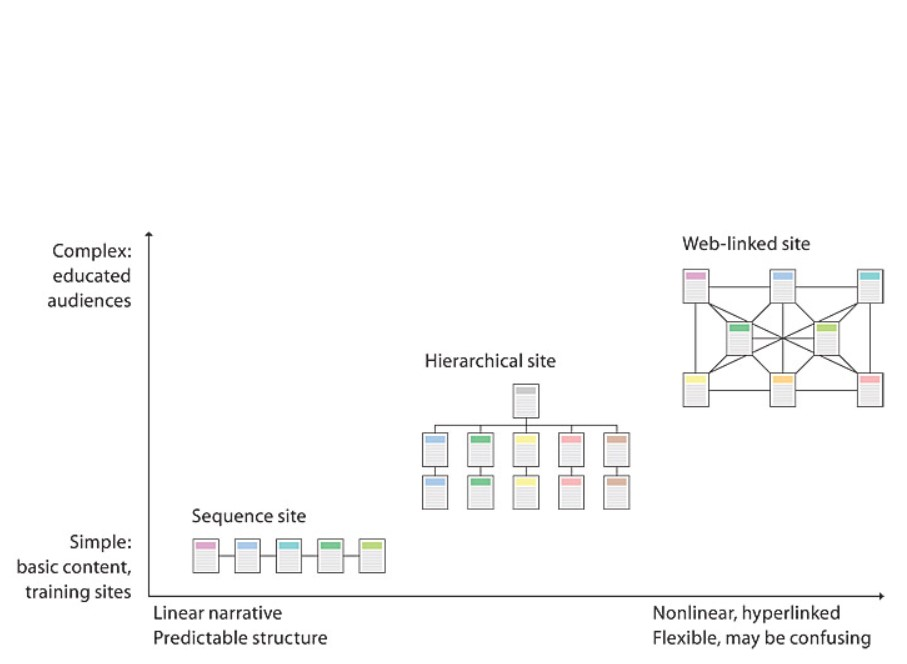
\includegraphics{images/netstruc_vs_hierstruc.jpg}
\caption{(\#fig:html\_tree)Linearity in Website Structure vs Audience Education}
\end{figure}

A \emph{second dimension} of hierarchy is brought by content architecture by means of the language used for content creation and organization i.e.~HTML. HTML stands for Hyper Text Markup Language and is the standard \emph{markup} language for documents designed to be showed into a web browser. It can be supported by technologies such as Cascading Style Sheets (CSS) and other scripting languages, as an example JavaScript \citep{html_2020}.
HTML inner language properties brings along the hierarchy that is then inherited from the website structure. According to this point of view the hierarchical website structure is a consequence of the language chosen for building content architecture.
Since a hierarchy structure is present a direction must be chosen, this direction is from root to leaves i.e.~\emph{arborescence}.
CSS language stands for Cascading Style Sheets and is a style sheet language used for modifying the appearance of a document written in a \emph{markup} language\citep{css_2020}.
The combination of HTML and CSS offers a wide flexibility in building web sites, once again expressed by the vast amount of different websites designs on the web. Some websites' components also might be tuned by a scripting language as Javascript. JavaScript enables interactive web pages and the vast majority of websites use it for all the operations that are performed by the client in a client-server relationship \citep{Javascript_2020}.
In the context of scraping Javascript adds a further layer of difficulty. As a matter of fact Javascript components are dynamic and scraping requires specialized libraries or remote web browser automation (\citep{RSelenium} R Bindings for Selenium 2.0 Remote WebDriver) to catch the website content.
CSS instead allows the scraper to target a class of objects in the web page that shares same style (e.g.~same CSS query) so that each element that belongs to the class (i.e.~share the same style) can be gathered. This practice provides tremendous advantages since by a single CSS query a precise set of objects can be obtained within a unique function call.
First and Second dimension of the scraping problem imply hierarchy. One way to imagine hierarchy in both of the two dimensions are graph based data structures named as \textbf{Rooted Trees}. By analyzing the first dimension through the lenses of Rooted trees it is possible to compress the whole setting into tree graph jargon, as a further reference on notation and wordings can be found in \citet{Graph_Diestel}. Rooted trees must start with a root node which in this context is the domain of the web page. Each \emph{Node} is a url destination and \emph{Edges} are the connections to web pages. Jumps from one page to the others (i.e.~connections) are possible in the website by nesting urls inside webpages so that within a single webpage the user can access to a limited number of other links. Each edge is associated to a \emph{Weight} whose interpretation is the run time cost to walk from one node to its connected others (i.e.~from a url to the other). In addition the content inside each node takes the name of payload, which is ultimately the goal of the scraping processes.
The walk from node ``body'' to node ``h2'' in figure below is called path and it represented as an ordered list of nodes connected by edges. In this context each node can have both a fixed and variable outgoing sub-nodes that are called \emph{Children} . When root trees have a fixed set of children are called \emph{k-ary} rooted trees. A node is said to be \emph{Parent} to other nodes when it is connected to them by outgoing edges, in the figure below ``headre'' is the parent of nodes ``h1'' and ``p''. Nodes in the tree that shares the same parent node are said \emph{Siblings}, ``h1'' and ``p'' are siblings in figure @ref(fig:html\_tree). Moreover \emph{Subtrees} are a set of nodes and edges comprised of a parent and its descendants e.g.~node ``main'' with all of its descendants might constitute a subtree. The concept of subtree in both of the problem dimensions plays crucial role in cutting run time scraping processes as well as fake headers provision (see section \ref{spoofing}). If the website strucuture is locally reproducible and the content architecture within webpages tends to be equal, then functions for a single subtree might be extended to the rest of others siblings subtrees. Local reproducibility is a property according to which starting from a single url all the related urls can be inferred from a pattern. Equal content architecture throughout different single links means to have a standard shared-within-webpages criteria according to which each single rental advertisement has to refer (e.g.~each new advertisement replicates the structure of the existing ones). In addition two more metrics describe the tree: \emph{level} and \emph{height}. The level of a node \(\mathbf{L}\) counts the number of edges on the path from the root node to \(\mathbf{L}\) , e.g.~``head'' and ``body'', are at the same level. The height is the maximum level for any node in the tree, from now on \(\mathbf{H}\), in figure @ref(fig:html\_tree). What is worth to be anticipating is that functions are not going to be applied directly to siblings in the ``upper'' general rooted tree (i.e.~from the domain). Instead the approach follwed is segmenting the highest tree into a sequence of single children unit that shares the same level (``nav'', ``main'', ``header'', ``title'' and ``footer'') for reasons explained in section \ref{spoofing}.

\begin{figure}
\centering
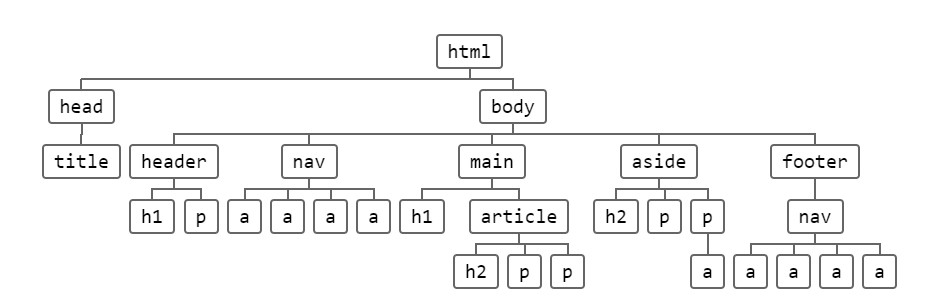
\includegraphics{images/html_general_representation.jpg}
\caption{(\#fig:html\_tree) html tree structure of a general website, randomly generated online}
\end{figure}

\hypertarget{webstructure}{%
\subsection{Immobiliare.it Webscraping website structure}\label{webstructure}}

The structure of immobiliare website can be assumed to be similar to the one of the largest online retailer Amazon. For that reason they both fall in the same website structure category. Sharing the same website structure category might imply that the transition from customized website structure scraping functions (i.e.~immobiliare) do not take too many sophistications to be extended to other comparables (i.e.~Amazon). Assuming that the scraper knows where are critical information (i.e.~payloads), what it takes to uncover the website structure is a way to decompose it. As a matter of fact each time the scraper script visits the website it should not to start back then from root node and down through the path straight to the bottom of the content. Indeed it should minimize the number of nodes encountered constrained to the respective weights. This is reached by engineering url composition.
According to some filters selected in a section (e.g.~city, number of rooms 5, square footage less than 60 \(m^2\) etc), the url is shaped so that each further filter is appended at the end of the domain url \texttt{https://www.immobiliare.it/} root node. Filters are appended with a proper syntax, not all the composition syntax are equal, that is why scraping script needs sophostication to be transalted from immobilaire to other websites in the same category. Once filters are all applied to the root domain this constitutes the new url root domain node that might have this appearance by filtering for rents in Milan city when square footage is less than 60 \(m^2\): domain +\texttt{affitto-case/milano/?superficieMinima=60}. Since this is true only for page n°1 containing the first 25 advs (see figure \ref{fig:websitetree}) all the remaining siblings nodes corresponding to the subsequent pages have to be generated. Here the utility of Local reproducibility property introduced in the previous section. The remaining siblings, i.e.~the ones belonging to page 2 (with the attached 25 links),to page 3 etc. can be generated by adding a further filter \texttt{\&pag=n}, where n is the page number reference (from now on referred as \emph{pagination}). Author customary choice is to stop pagination up to 300 pages since spatial data can not be to too large due to computational constraints imposed by inla methodology \ref{inla}.
Up to this point pagination has generated a vector of siblings nodes whose children elements number is fixed (i.e.~25 links per page \ref{fig:websitetree} lower part). That makes those trees \emph{k-ary}, where k is 25 indicating the number of children leaves. K-ary trees are rooted trees in which each node has no more than k children, in this particular case final leaves. The well known binary rooted tree is actually a special case of k-ary when \(k = 2\). Filters reverse engineering process and 25-ary trees with equal content structure across siblings allow to design a single function to call that could be mapped for all the other siblings. In addition in order to further unroll the website a specific scraping function grabs the whole set of 25 links per page. As a result a single function call of \texttt{scrape\_href()} can grab the links corresponding to page 1. Then the function is mapped for all the generated siblings nodes (i.e.~up to 300) obtaining a collection of all links belonging to the set of pages. Ultimately the complete set of links corresponds to every single advertisement posted on immobiliare.it at a given time.

\begin{figure}
\centering
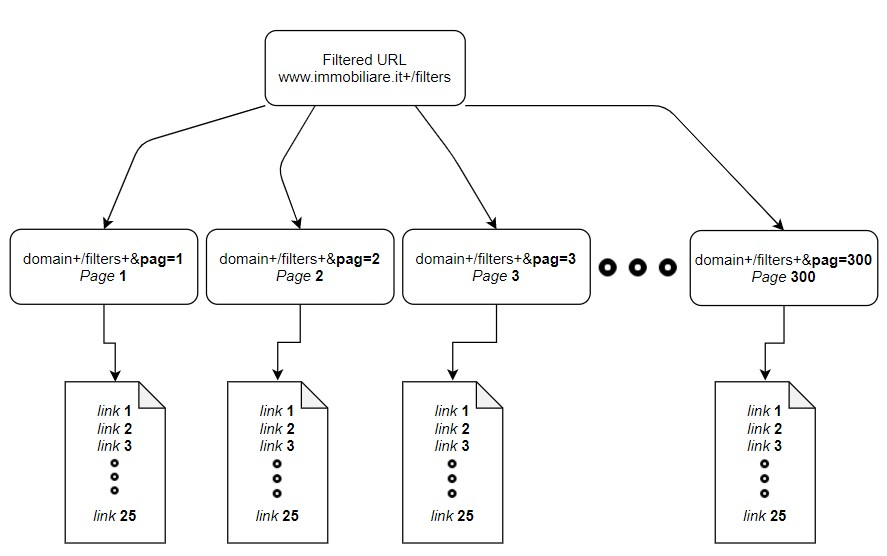
\includegraphics{images/website_tree1.jpg}
\caption{\label{fig:websitetree}immobiliare.it website structure, author's source}
\end{figure}

\hypertarget{immobiliare.it-webscraping-content-architecture-with-rvest}{%
\subsection{\texorpdfstring{Immobiliare.it Webscraping content architecture with \texttt{rvest}}{Immobiliare.it Webscraping content architecture with rvest}}\label{immobiliare.it-webscraping-content-architecture-with-rvest}}

To start a general scraping function the only requirements are a target url (i.e.~the filtered root node url) and a way to compose url (i.e.~pagination ). Then a session class object \texttt{html\_session} is opened by specifying the url and the request data that the user needs to send to the web server, see left part to dashed line in figure \ref{fig:workflow}. Information to be attached to the web server request will be further explored later, tough they are mainly three: User Agents, emails references and proxy servers. \texttt{html\_session} class objects contains a list number of useful data such as: the url, the response, cookies, session times etc. Once the connection is established (response request 200) all the following operations rely on the opened session, in other words for the time being in the session the user will be authorized with the already provided request data. The list object contains the xml/html content response of the webpage and that is where data needs to be parsed and class converted. The list can disclose as well other interesting meta information related to the session but in this context are not collected. The light blue wavy line follows the steps required to get the content parsed from the beginning to the end.

\begin{figure}
\centering
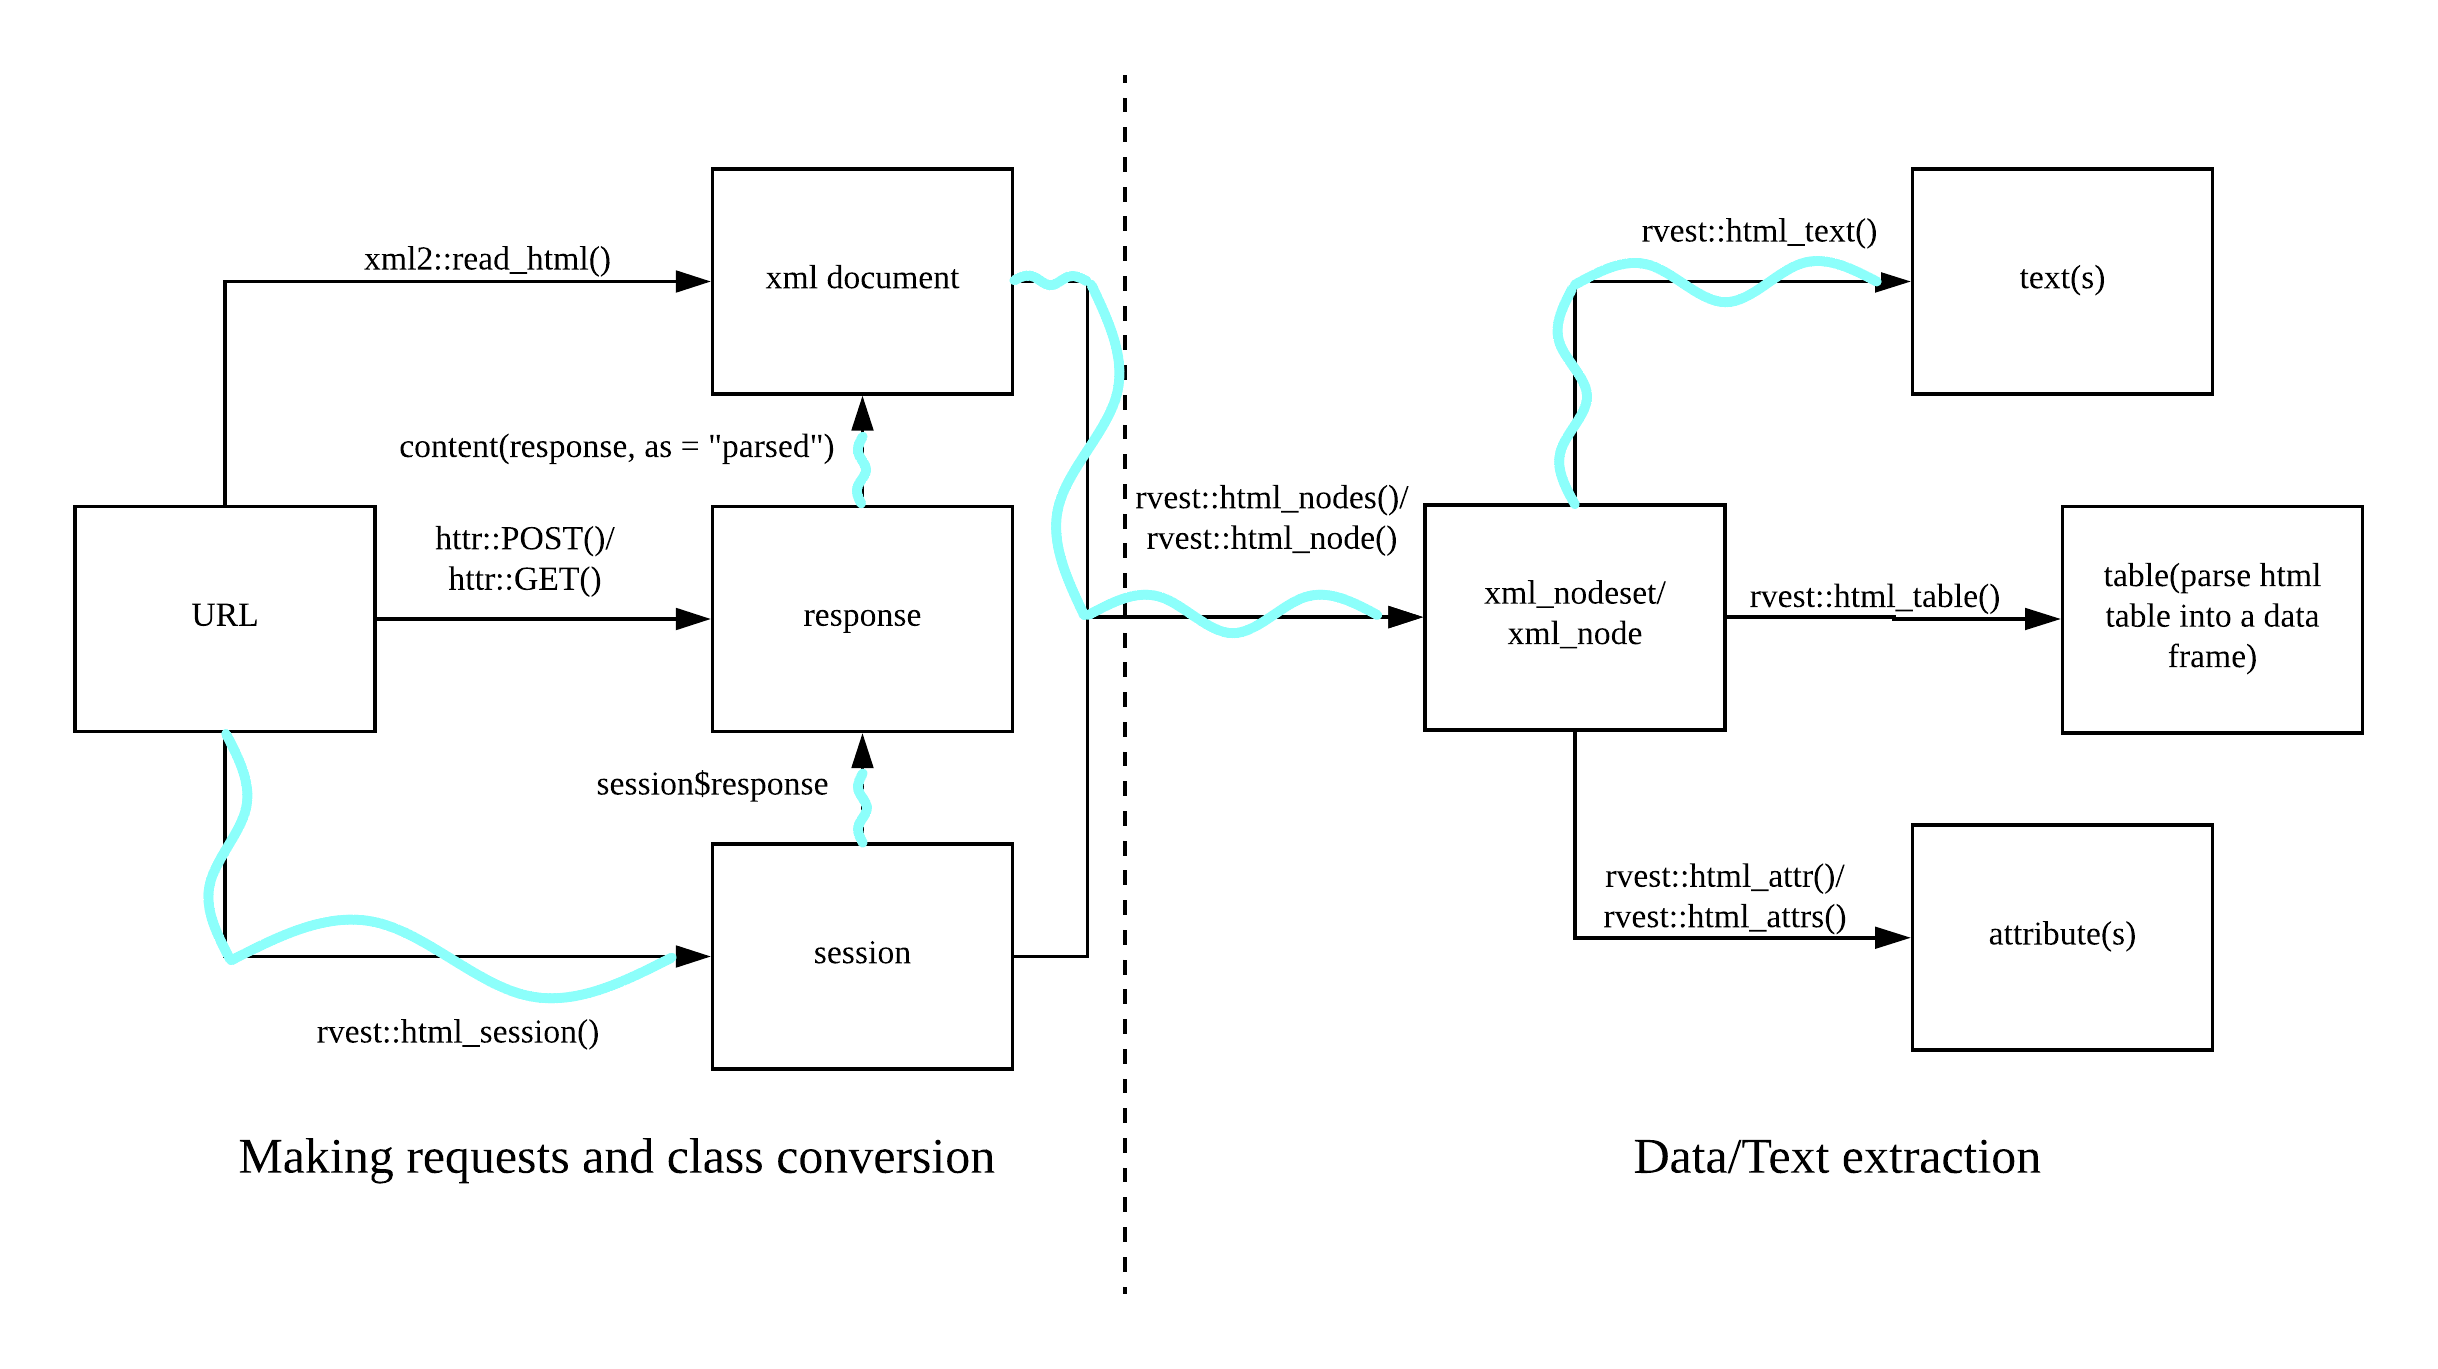
\includegraphics{images/workflow.png}
\caption{\label{fig:workflow}rvest general flow chart, author's source}
\end{figure}

To the right of dashed line in the flow chart \ref{fig:workflow} are painted a sequence of \texttt{rvest}\citep{rvest} functions that follow a general step by step text comprehension rules. \texttt{rvest} first handles parsing the html respose content of the web page within the session through \texttt{read\_html()}. Secondly, as in figure \ref{fig:ContentStructure}, it looks for a single node \texttt{html\_nodes()} through a specified CSS query. CSS is a way to route \texttt{rvest} to consider a precise node or set of nodes in the web page. For each information contained in each of the web page a different CSS query has to be called.
Thirdly it converts the content (i.e.~payload) into a human readable text with \texttt{html\_text()}. A simplified version of the important contents to be scraped in each single link is sketched in figure \ref{fig:ContentStructure}

\begin{figure}
\centering
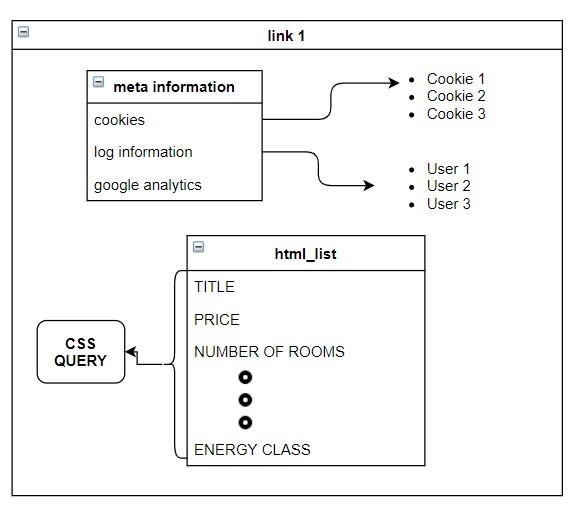
\includegraphics{images/content_structure.jpg}
\caption{\label{fig:ContentStructure}immobiliare.it important content structure, author's source}
\end{figure}

The code chunk below exemplifies a function that can scrape the price. The function explicitly covers only the right part to the dashed line (figure \ref{fig:workflow}) of the whole scraping process. The initial part (left dashed in same figure), where session is opened and response is converted is handles inside the second code chunk where \texttt{get.data.catsing()} is.

\begin{Shaded}
\begin{Highlighting}[]
\NormalTok{scrapeprice.imm =}\StringTok{ }\ControlFlowTok{function}\NormalTok{(session) \{}
    
\NormalTok{    opensess =}\StringTok{ }\KeywordTok{read_html}\NormalTok{(session)}
\NormalTok{    price =}\StringTok{ }\NormalTok{opensess }\OperatorTok\StringTok{ }\KeywordTok{html_nodes}\NormalTok{(}\DataTypeTok{css =} \StringTok{".im-mainFeatures__title"}\NormalTok{) }\OperatorTok\StringTok{ }\KeywordTok{html_text}\NormalTok{() }\OperatorTok\StringTok{ }
\StringTok{        }\KeywordTok{str_trim}\NormalTok{()}
    
    \ControlFlowTok{if}\NormalTok{ (}\KeywordTok{is.null}\NormalTok{(price) }\OperatorTok{||}\StringTok{ }\KeywordTok{identical}\NormalTok{(price, }\KeywordTok{character}\NormalTok{(}\DecValTok{0}\NormalTok{))) \{}
\NormalTok{        price2 =}\StringTok{ }\NormalTok{opensess }\OperatorTok\StringTok{ }\KeywordTok{html_nodes}\NormalTok{(}\DataTypeTok{css =} \StringTok{".im-features__value , .im-features__title"}\NormalTok{) }\OperatorTok\StringTok{ }
\StringTok{            }\KeywordTok{html_text}\NormalTok{() }\OperatorTok\StringTok{ }\KeywordTok{str_trim}\NormalTok{()}
        
        \ControlFlowTok{if}\NormalTok{ (}\StringTok{"prezzo"} \OperatorTok\StringTok{ }\NormalTok{price2) \{}
\NormalTok{            pos =}\StringTok{ }\KeywordTok{match}\NormalTok{(}\StringTok{"prezzo"}\NormalTok{, price2)}
            \KeywordTok{return}\NormalTok{(price2[pos }\OperatorTok{+}\StringTok{ }\DecValTok{1}\NormalTok{]) }\OperatorTok\StringTok{ }\KeywordTok{str_replace_all}\NormalTok{(}\KeywordTok{c}\NormalTok{(}\StringTok{`}\DataTypeTok{\textbackslash{}200}\StringTok{`}\NormalTok{ =}\StringTok{ ""}\NormalTok{, }\StringTok{`}\CharTok{\textbackslash{}\textbackslash{}}\DataTypeTok{.}\StringTok{`}\NormalTok{ =}\StringTok{ ""}\NormalTok{)) }\OperatorTok\StringTok{ }
\StringTok{                }\KeywordTok{str_extract}\NormalTok{(}\StringTok{"}\CharTok{\textbackslash{}\textbackslash{}}\StringTok{-*}\CharTok{\textbackslash{}\textbackslash{}}\StringTok{d+}\CharTok{\textbackslash{}\textbackslash{}}\StringTok{.*}\CharTok{\textbackslash{}\textbackslash{}}\StringTok{d*"}\NormalTok{) }\OperatorTok\StringTok{ }\KeywordTok{str_replace_na}\NormalTok{() }\OperatorTok\StringTok{ }\KeywordTok{str_replace}\NormalTok{(}\StringTok{"NA"}\NormalTok{, }
                \StringTok{"Prezzo Su Richiesta"}\NormalTok{)}
\NormalTok{        \} }\ControlFlowTok{else}\NormalTok{ \{}
            \KeywordTok{return}\NormalTok{(}\OtherTok{NA_character_}\NormalTok{)}
\NormalTok{        \}}
\NormalTok{    \} }\ControlFlowTok{else}\NormalTok{ \{}
        \KeywordTok{return}\NormalTok{(price) }\OperatorTok\StringTok{ }\KeywordTok{str_replace_all}\NormalTok{(}\KeywordTok{c}\NormalTok{(}\StringTok{`}\DataTypeTok{\textbackslash{}200}\StringTok{`}\NormalTok{ =}\StringTok{ ""}\NormalTok{, }\StringTok{`}\CharTok{\textbackslash{}\textbackslash{}}\DataTypeTok{.}\StringTok{`}\NormalTok{ =}\StringTok{ ""}\NormalTok{)) }\OperatorTok\StringTok{ }\KeywordTok{str_extract}\NormalTok{(}\StringTok{"}\CharTok{\textbackslash{}\textbackslash{}}\StringTok{-*}\CharTok{\textbackslash{}\textbackslash{}}\StringTok{d+}\CharTok{\textbackslash{}\textbackslash{}}\StringTok{.*}\CharTok{\textbackslash{}\textbackslash{}}\StringTok{d*"}\NormalTok{) }\OperatorTok\StringTok{ }
\StringTok{            }\KeywordTok{str_replace_na}\NormalTok{() }\OperatorTok\StringTok{ }\KeywordTok{str_replace}\NormalTok{(}\StringTok{"NA"}\NormalTok{, }\StringTok{"Prezzo Su Richiesta"}\NormalTok{)}
        
\NormalTok{    \}}
\NormalTok{\}}
\end{Highlighting}
\end{Shaded}

The function takes as a single argument a session object, then It reads the inner html content in the session storing the information into an obj called the \texttt{opensess}. Another obj is created, namely price, right after the pipe operator a CSS query into the html is called. The CSS query \texttt{.im-mainFeatures\_\_title} points to a precise group of data inside the web page, right below the main title. Expectation are that price is a one-element chr vector, containing the price and other unnecessary non-UTF characters. Then the algorithm enters into the first \texttt{if} statement. The handler checks if the object \texttt{price} is empty. If it doesn't the algorithm jumps to the end of the function and returns the quantity cleaned. But If it does it takes again the \texttt{opensess} and tries with a second css query \texttt{.im-features\_\_value\ ,\ .im-features\_\_title} in a second data location where price might be also found. Please note that this is all done within the same session, so no more additional request information has to be sent. Since the latter CSS query points to data stored inside a list object, for the time being the newly created \texttt{price2} is a list containing various information. Then the algorithm flow enters into the second \texttt{if} statement that checks whether \texttt{"prezzo"} is matched the list or not, if it does it returns the +1 position index element with respect to the ``prezzo'' positioning. This happens because data in price2 list are stored by couples sequentially, e.g.~{[}title, ``Appartamento Sempione'', energy class, ``G'', ``prezzo'', 1200/al mese{]}. When it returns the element corresponding to +1 position index it applies also some data wrangling with \texttt{stringr} package to keep out overabundant characters. The function then escapes in the else statement by setting \texttt{price2\ =\ NA\_Character\_} once no CSS query could be finding the price information. the \emph{NA-character-string} type has to be imposed due to fact that later they can not be bind. In other words if the function is evaluated for a url and returns the price quantity, but then is evaluated for url2 and outputs NA (no character) then results can not be combined into dataframe due to different object types.

Once all the functions have been created they need to be called together and then data coming after them need to be combined. This is done by \texttt{get.data.catsing()} which at first checks the validity of the url, then takes the same url as input and filters it as a session object. Then simultaneously all the functions are called and then combined. All this happens inside a \texttt{foreach} parallel loop called by \texttt{scrape.all.info()}

\begin{Shaded}
\begin{Highlighting}[]
\NormalTok{scrape.all.info =}\StringTok{ }\ControlFlowTok{function}\NormalTok{(}\DataTypeTok{url =} \StringTok{"https://www.immobiliare.it/affitto-case..."}\NormalTok{,}
                           \DataTypeTok{vedi =} \OtherTok{FALSE}\NormalTok{, }
                           \DataTypeTok{scrivi =} \OtherTok{FALSE}\NormalTok{, }
                           \DataTypeTok{silent =} \OtherTok{FALSE}\NormalTok{)\{}
  \ControlFlowTok{if}\NormalTok{ (silent) \{}
\NormalTok{    start =}\StringTok{ }\KeywordTok{as_hms}\NormalTok{(}\KeywordTok{Sys.time}\NormalTok{()); }\KeywordTok{cat}\NormalTok{(}\StringTok{'Starting the process...}\CharTok{\textbackslash{}n\textbackslash{}n}\StringTok{'}\NormalTok{)}
    \KeywordTok{message}\NormalTok{(}\StringTok{'}\CharTok{\textbackslash{}n}\StringTok{The process has started in'}\NormalTok{,}\KeywordTok{format}\NormalTok{(start,}\DataTypeTok{usetz =} \OtherTok{TRUE}\NormalTok{))  }
\NormalTok{  \}}
  \CommentTok{# open parallel multisession }
\NormalTok{  cores =}\KeywordTok{detectCores}\NormalTok{(}\DataTypeTok{logical =} \OtherTok{FALSE}\NormalTok{)}
\NormalTok{  cl =}\StringTok{ }\KeywordTok{makeCluster}\NormalTok{(cores)}
  \KeywordTok{registerDoParallel}\NormalTok{(cl,cores)}
\NormalTok{  start =}\StringTok{ }\KeywordTok{as_hms}\NormalTok{(}\KeywordTok{Sys.time}\NormalTok{())}
  
  \ControlFlowTok{if}\NormalTok{ (silent) \{}
    \KeywordTok{message}\NormalTok{(}\StringTok{'}\CharTok{\textbackslash{}n\textbackslash{}n}\StringTok{Start all the requests at time:'}\NormalTok{, }\KeywordTok{format}\NormalTok{(start,}\DataTypeTok{usetz =}\NormalTok{ T))  }
\NormalTok{  \}}
\NormalTok{  ALL =}\StringTok{ }\KeywordTok{foreach}\NormalTok{(}\DataTypeTok{i =} \KeywordTok{seq_along}\NormalTok{(links),}
                \DataTypeTok{.packages =}\NormalTok{ lista.pacchetti,}
                \DataTypeTok{.combine =} \StringTok{"bind_rows"}\NormalTok{,}
                \DataTypeTok{.multicombine =} \OtherTok{FALSE}\NormalTok{,}
                \DataTypeTok{.export =}\StringTok{"links"}\NormalTok{ ,}
                \DataTypeTok{.verbose =} \OtherTok{TRUE}\NormalTok{,}
                \DataTypeTok{.errorhandling=}\StringTok{'pass'}\NormalTok{) }\OperatorTok\StringTok{ }\NormalTok{\{}
                  \KeywordTok{source}\NormalTok{(}\StringTok{"utils.R"}\NormalTok{)}
                  \KeywordTok{sourceEntireFolder}\NormalTok{(}\StringTok{"functions_singolourl"}\NormalTok{)}
\NormalTok{                  get.data.catsing =}\StringTok{ }\ControlFlowTok{function}\NormalTok{(singolourl)\{}
                    
                    \CommentTok{# dormi()}
                    \CommentTok{# }
                    \ControlFlowTok{if}\NormalTok{(}\OperatorTok{!}\KeywordTok{is_url}\NormalTok{(singolourl))\{}
                      \KeywordTok{stop}\NormalTok{(}\KeywordTok{paste0}\NormalTok{(}\StringTok{"The following url does not seem either to exist or it is invalid"}\NormalTok{, singolourl))}
\NormalTok{                    \}}
                    
\NormalTok{                    session =}\StringTok{ }\KeywordTok{html_session}\NormalTok{(singolourl, }\KeywordTok{user_agent}\NormalTok{(agents[}\KeywordTok{sample}\NormalTok{(}\DecValTok{1}\NormalTok{)]))}
                    \ControlFlowTok{if}\NormalTok{ (}\KeywordTok{class}\NormalTok{(session) }\OperatorTok{==}\StringTok{ "session"}\NormalTok{) \{}
\NormalTok{                      session =}\StringTok{ }\NormalTok{session}\OperatorTok{$}\NormalTok{response  }
\NormalTok{                    \}}
                      
\NormalTok{                    id         =}\StringTok{ }\KeywordTok{tryCatch}\NormalTok{(\{}\KeywordTok{scrapehouse.ID}\NormalTok{(session)\},}
                                          \DataTypeTok{error =} \ControlFlowTok{function}\NormalTok{(e)\{ }\KeywordTok{message}\NormalTok{(}\StringTok{"some problem occured in scrapehouse.ID"}\NormalTok{) \})}
\NormalTok{                    lat        =}\StringTok{ }\KeywordTok{tryCatch}\NormalTok{(\{}\KeywordTok{scrapelat.imm}\NormalTok{(session)\},}
                                          \DataTypeTok{error =} \ControlFlowTok{function}\NormalTok{(e)\{ }\KeywordTok{message}\NormalTok{(}\StringTok{"some problem occured in scrapelat.imm"}\NormalTok{) \})}
\NormalTok{                    long       =}\StringTok{ }\KeywordTok{tryCatch}\NormalTok{(\{}\KeywordTok{scrapelong.imm}\NormalTok{(session)\},}
                                          \DataTypeTok{error =} \ControlFlowTok{function}\NormalTok{(e)\{ }\KeywordTok{message}\NormalTok{(}\StringTok{"some problem occured in scrapelong.imm"}\NormalTok{) \})}
\NormalTok{                    location   =}\StringTok{ }\KeywordTok{tryCatch}\NormalTok{(\{}\KeywordTok{take.address}\NormalTok{(session)\},}
                                          \DataTypeTok{error =} \ControlFlowTok{function}\NormalTok{(e)\{ }\KeywordTok{message}\NormalTok{(}\StringTok{"some problem occured in take.address"}\NormalTok{) \})}
\NormalTok{                    condom     =}\StringTok{ }\KeywordTok{tryCatch}\NormalTok{(\{}\KeywordTok{scrapecondom.imm}\NormalTok{(session)\},}
                                          \DataTypeTok{error =} \ControlFlowTok{function}\NormalTok{(e)\{ }\KeywordTok{message}\NormalTok{(}\StringTok{"some problem occured in scrapecondom.imm"}\NormalTok{) \})}
\NormalTok{                    buildage   =}\StringTok{ }\KeywordTok{tryCatch}\NormalTok{(\{}\KeywordTok{scrapeagebuild.imm}\NormalTok{(session)\},}
                                          \DataTypeTok{error =} \ControlFlowTok{function}\NormalTok{(e)\{ }\KeywordTok{message}\NormalTok{(}\StringTok{"some problem occured in scrapeagebuild.imm"}\NormalTok{) \})}
                    
\NormalTok{                  ...}
                  
\NormalTok{                   combine =}\StringTok{ }\KeywordTok{tibble}\NormalTok{(}\DataTypeTok{ID        =}\NormalTok{ id,}
                                     \DataTypeTok{LAT       =}\NormalTok{ lat, }
                                     \DataTypeTok{LONG      =}\NormalTok{ long,}
                                     \DataTypeTok{LOCATION  =}\NormalTok{ location,}
                                     \DataTypeTok{CONDOM    =}\NormalTok{ condom,}
                                     \DataTypeTok{BUILDAGE  =}\NormalTok{ buildage,}
                                    
\NormalTok{                  ...}
                  
                  
                  \KeywordTok{return}\NormalTok{(combine)}
                  \ErrorTok{\}}
  \KeywordTok{stopImplicitCluster}\NormalTok{()                 }
  \KeywordTok{stopCluster}\NormalTok{(cl)}
  \KeywordTok{return}\NormalTok{(ALL)}
\ErrorTok{\}}
\end{Highlighting}
\end{Shaded}

The skeleton used for price constitutes a standard format adopted for many other scraping function in the analysis. Being equal the CSS query what it changes is the matching term, i.e.~``numero camere'' instead of ``prezzo'' to look for how many rooms there are in the house. This is true for all the information contained in the list accessed by the fixed css query. Those that are not they are a few and they do not need to be scraped.
In addition some other functions outputs need to undergo to further heavy cleaning steps in order to be usable As a consequence of that functions need also to be broken down by pieces by single .R files, whose names correspond to each important information.
Below it is printed the tree structure folder that composes the main elements of the scraping procedure. It can be noticed that the two folders, namely functions\_singolourl and functions\_url enclose all the single functions that allows to grab each information from the session. Folders with a customized function are then sourced within the two main functions, scrape.all and scrape.all.info so data can be extracted.

\begin{verbatim}
 levelName
1  immobiliare.it-WebScraping     
2   ¦--functions_singolourl       
3   ¦   ¦--0scrapesqfeetINS.R     
4   ¦   ¦--0scrapenroomINS.R      
5   ¦   ¦--0scrapepriceINS.R      
6   ¦   ¦--0scrapetitleINS.R      
7   ¦   ¦--ScrapeAdDate.R         
8   ¦   ¦--ScrapeAge.R            
9   ¦   ¦--ScrapeAgeBuilding.R    
10  ¦   ¦--ScrapeAirConditioning.R
11  ¦   ¦--ScrapeAptChar.R        
12  ¦   ¦--ScrapeCatastInfo.R     
13  ¦   ¦--ScrapeCompart.R        
14  ¦   ¦--ScrapeCondom.R         
15  ¦   ¦--ScrapeContr.R          
16  ¦   ¦--ScrapeDisp.R           
17  ¦   ¦--ScrapeEnClass.R        
18  ¦   ¦--ScrapeFloor.R          
19  ¦   ¦--ScrapeHasMulti.R       
20  ¦   ¦--ScrapeHeating.R        
21  ¦   ¦--ScrapeHouseID.R        
22  ¦   ¦--ScrapeHouseTxtDes.R    
23  ¦   ¦--ScrapeLAT.R            
24  ¦   ¦--ScrapeLONG.R           
25  ¦   ¦--ScrapeLoweredPrice.R   
26  ¦   ¦--ScrapeMetrature.R      
27  ¦   ¦--ScrapePhotosNum.R      
28  ¦   ¦--ScrapePostAuto.R       
29  ¦   ¦--ScrapePropType.R       
30  ¦   ¦--ScrapeReaReview.R      
31  ¦   ¦--ScrapeStatus.R         
32  ¦   ¦--ScrapeTotPiani.R       
33  ¦   ¦--ScrapeType.R           
34  ¦   °--take_location.R        
35  ¦--scrapeALL.R                
36  ¦--scrapeALLINFO.R            
37  ¦--functions_url              
38  ¦   ¦--ScrapeHREF.R           
39  ¦   ¦--ScrapePrice.R          
40  ¦   ¦--ScrapePrimaryKey.R     
41  ¦   ¦--ScrapeRooms.R          
42  ¦   ¦--ScrapeSpace.R          
43  ¦   °--ScrapeTitle.R          
44  ¦--libs.R                     
45  ¦--utils.R                    
46  ¦--README.Rmd                 
47  ¦--README.md                  
48  °--simulations                
49      ¦--rt_match_vs_forloop.R  
50      °--runtime_simul.R
\end{verbatim}

\hypertarget{best-practices}{%
\section{Scraping Best Practices and Security provisions}\label{best-practices}}

Robots.txt files are (rivedi citation) a way to kindly ask webbots, spiders, crawlers, wanderers to access or not access certain parts of a webpage. The de facto `standard' never made it beyond a informal ``Network Working Group INTERNET DRAFT''. Nonetheless, the use of robots.txt files is widespread (e.g.~\url{https://en.wikipedia.org/robots.txt}, \url{https://www.google.com/robots.txt}) and bots from Google, Yahoo adhere to the rules defined in robots.txt files, although their \emph{interpretation} of those rules might differ.

Robots.txt files are plain text and always found at the root of a website's domain. The syntax of the files in essence follows a field-name value scheme with optional preceding user-agent. Blocks are separated by blank lines and the omission of a user-agent field (which directly corresponds to the HTTP user-agent field) is seen as referring to all bots. \# serves to comment lines and parts of lines. Everything after \# until the end of line is regarded a comment. Possible field names are: user-agent, disallow, allow, crawl-delay, sitemap, and host. For further references on robotstxt are recommended \citep[\citet{google:robottxt}]{robotstxt}.

Some interpretation problems:

\begin{itemize}
\tightlist
\item
  Finding no robots.txt file at the server (e.g.~HTTP status code 404) implies that everything is permitted.
\item
  Subdomains should have there own robots.txt file if not it is assumed that everything is allowed.
\item
  Redirects from subdomain www to the doamin is considered no domain change - so whatever is found at the end of the redirect is considered to be the robots.txt file for the subdomain originally requested.
\end{itemize}

For the thesis purposes it has been designed a dedicated function to assess whether the domain or the related paths require specific actions or they prevent some activity on the target. The following \texttt{checkpermission()} function has been integrated inside the scraping system and it is called once at the starting point.

\begin{Shaded}
\begin{Highlighting}[]
\NormalTok{dominio =}\StringTok{ "immobiliare.it"}

\NormalTok{checkpermission =}\StringTok{ }\ControlFlowTok{function}\NormalTok{(dom) \{}
    
\NormalTok{    robot =}\StringTok{ }\KeywordTok{robotstxt}\NormalTok{(}\DataTypeTok{domain =}\NormalTok{ dom)}
\NormalTok{    vd =}\StringTok{ }\NormalTok{robot}\OperatorTok{$}\KeywordTok{check}\NormalTok{()[}\DecValTok{1}\NormalTok{]}
    \ControlFlowTok{if}\NormalTok{ (vd) \{}
        \KeywordTok{cat}\NormalTok{(}\StringTok{"}\CharTok{\textbackslash{}n}\StringTok{robot.txt for"}\NormalTok{, dom, }\StringTok{"is okay with scraping!"}\NormalTok{)}
\NormalTok{    \} }\ControlFlowTok{else}\NormalTok{ \{}
        \KeywordTok{cat}\NormalTok{(}\StringTok{"}\CharTok{\textbackslash{}n}\StringTok{robot.txt does not like what you're doing"}\NormalTok{)}
        \KeywordTok{stop}\NormalTok{()}
\NormalTok{    \}}
\NormalTok{\}}
\CommentTok{## metti path allowed check}
\KeywordTok{checkpermission}\NormalTok{(dominio)}
\end{Highlighting}
\end{Shaded}

\begin{verbatim}
## 
## robot.txt for immobiliare.it is okay with scraping!
\end{verbatim}

Further improvements in this direction might come with the \texttt{polite} package \citep{polite} which combines the power of the \texttt{robotstxt}, the \texttt{ratelimitr} \citep{ratelimitr} to limit sequential requests together with the \texttt{memoise} \citep{memoise} for response caching. This package is wrapped up around 3 simple but effective ideas:

\begin{quote}
The three pillars of a polite session are seeking permission, taking slowly and never asking twice.
\end{quote}

The three pillars constitute the \emph{Ethical} web scraping manifesto \citep{densmore_2019} which are common shared practises that are aimed to self regularize scrapers. These have to be intended as best practices, not in any case as law enforcements, however many scrapers themselves, as website administrators or analyst, have fought in their daily working tasks with bots. Crawling bots in intensive scraping processes might fake real client navigation logs and as a consequence might induce distorted analytics. Due to this fact comes the need to find a common operating ground and therefore politely asking for permission.

\hypertarget{security-provisions-user-agents-proxies-and-handlers}{%
\section{Security provisions: User Agents, Proxies and Handlers}\label{security-provisions-user-agents-proxies-and-handlers}}

HTTP requests to the website server by web clients come with some mandatory information packed in it. The process according to which HTTP protocols allow to exchange information can be easily thought with an everyday real world analogy. As a generic person A rings the door's bell of person B's house. A comes to B door with its personal information, its name, surname, where he lives etc. At this point B may either answer to A requests by opening the door and let him enter given the set of information he has, or it may not since B is not sure of the real intentions of A. This typical everyday situation in nothing more what happens billions of times on the internet everyday, the user browser (in the example above A) is interacting with a server website (part B) sending packets of information, figure \ref{fig:webworks}. If a server does not trust the information provided by the user, if the requests are too many, if the requests seems to be scheduled due to fixed sleeping time, a server can block requests. In certain cases it can even forbid the user log to the website. The language the two parties exchanges are coded in numbers that ranges from 100 to 511, each of which has its own specific significance. A popular case of this type of interaction occurs when users are not connected to internet so the server responds 404, page not found. Servers are built with a immune-system like software that raises barriers and block users to prevent dossing or other illegal practices.

\begin{figure}
\centering
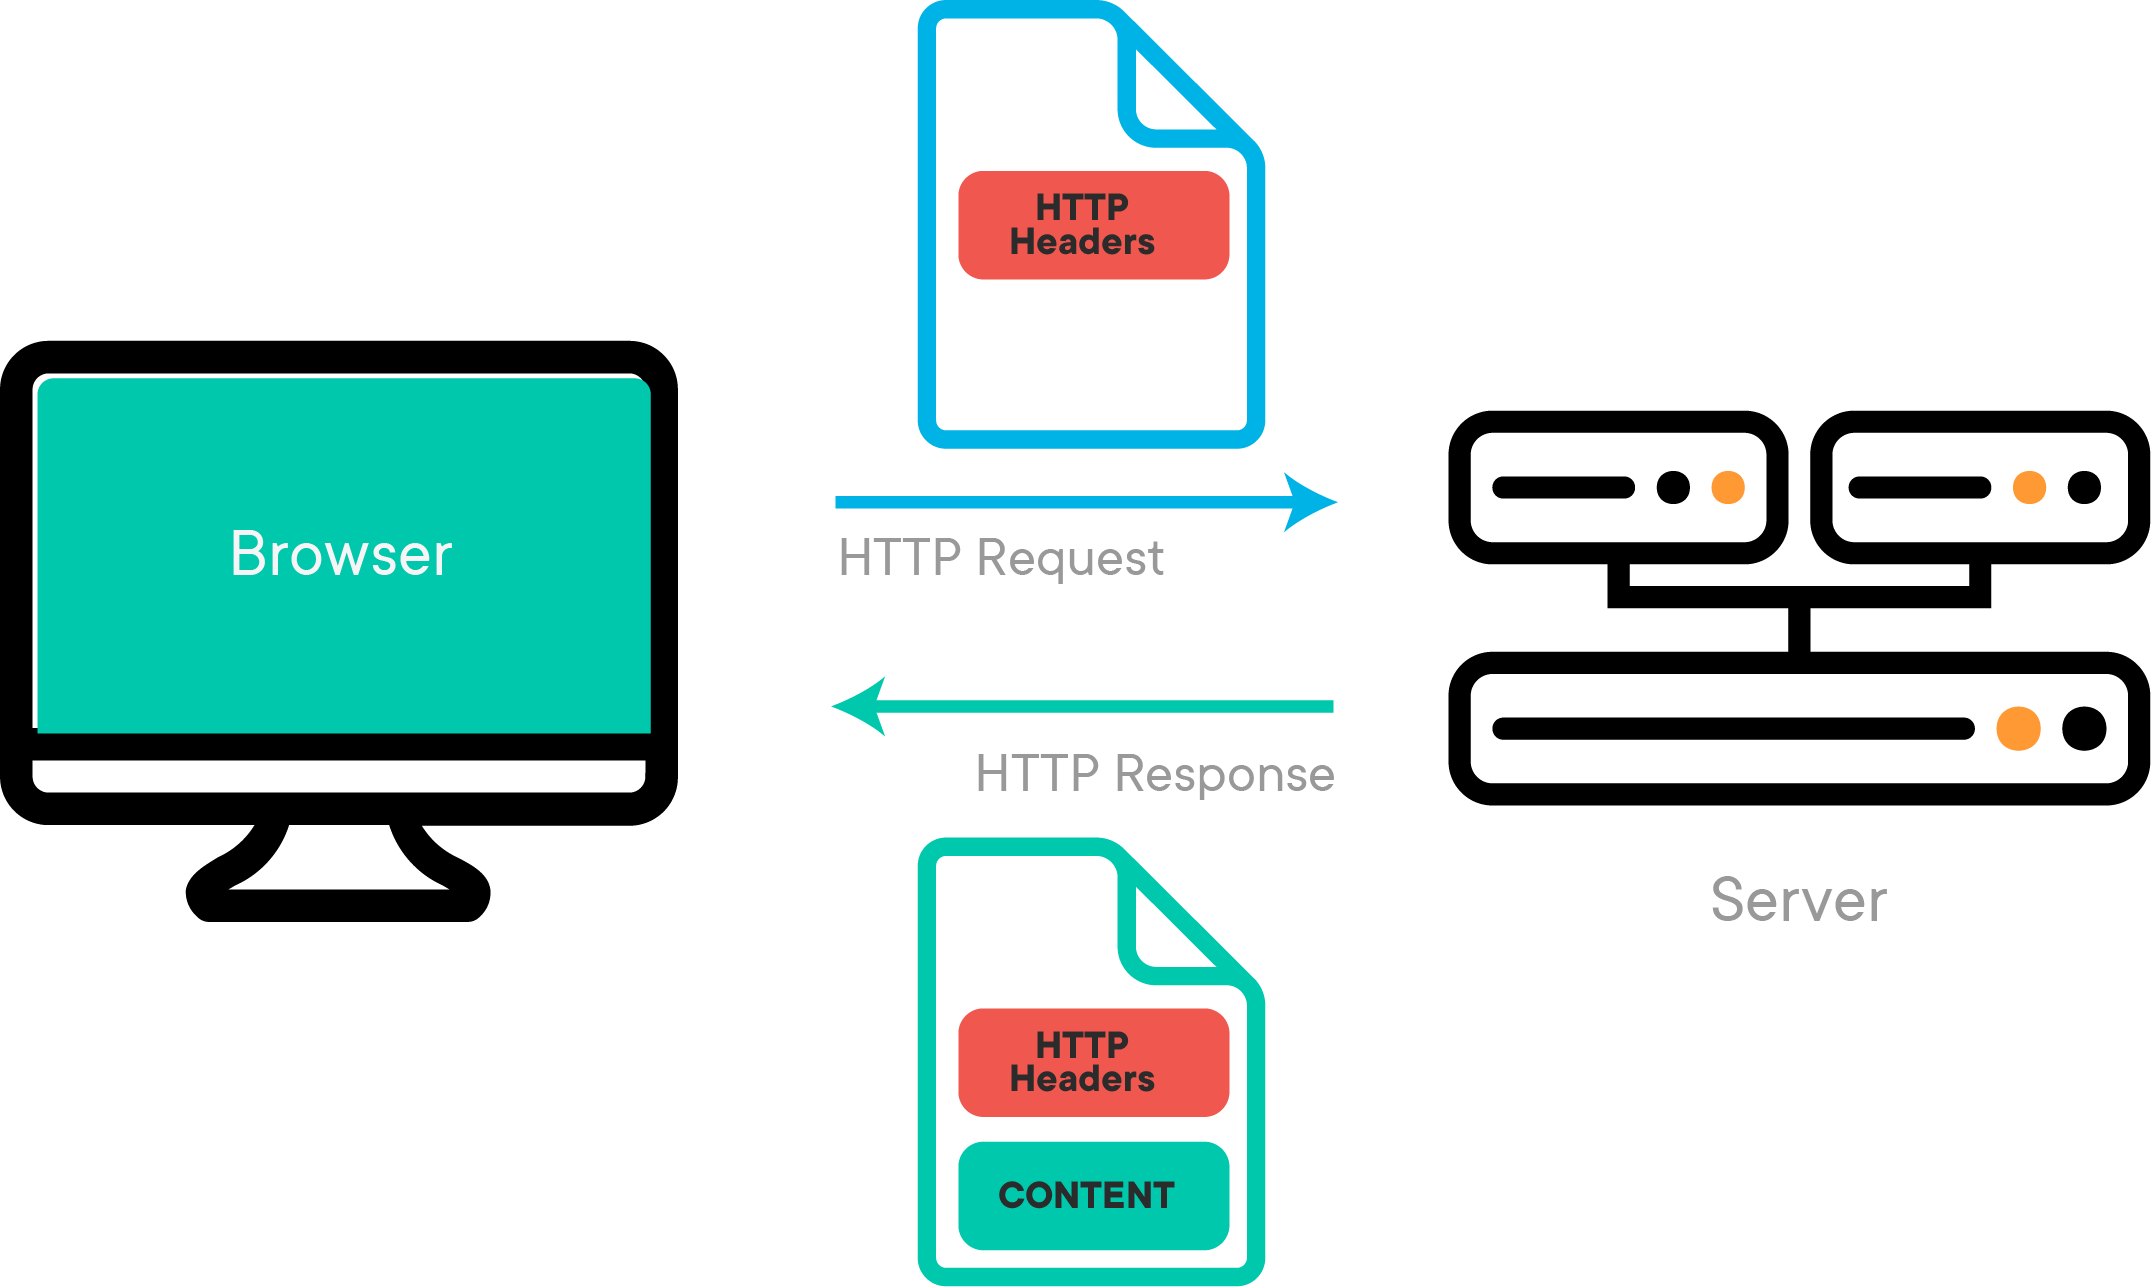
\includegraphics{images/how_web_works.png}
\caption{\label{fig:webworks}How the web interacts between broswer and server}
\end{figure}

This procedure is a daily issue to scraper that are trying to collect information from websites. Google performs it everyday with its spider crawlers, which are very sophisticated bots that scrapes over a enormous range of websites. This challenge can be addressed in multiple ways, there are some specific Python packages that overcome this issue. Precautions have not been taken lightly, and a simple but effective approach is proposed.

\hypertarget{spoofing}{%
\subsection{User Agents Spoofing}\label{spoofing}}

\begin{definition}[User Agents]
\protect\hypertarget{def:useragents}{}{\label{def:useragents} \iffalse (User Agents) \fi{} }A user agent \citep{whoishostingthis.com} is a string of characters in each web browser that serves as identification card. The user agent permits the web server to be able to identify the user operating system and the browser. Then, the web server uses the exchanged information to determine what content should be presented to particular operating systems and web browsers on a series of devices.
\end{definition}

The user agent string includes the user application or software, the operating system (and their versions), the web client, the web client's version, as well as the web engine responsible for the content display (such as AppleWebKit). The user agent string is sent in the form of a HTTP request header. Since User Agents acts as middle man between the client request and the server response, then from a continuous scraping point of view it would be better rotating them, so that each time the middle man looks different. The solution adopted builds a vector of user agent strings identified by different specifications, different web client, different operating system and so on, then samples 1 of them
Then whenever a request from a web browser is sent to a web server, 1 random sample string is drawn from the user agents pool. So each time the user is sending the request it appears to be a different User Agent.
Below the user agents rotation pool:

\begin{Shaded}
\begin{Highlighting}[]
\KeywordTok{set.seed}\NormalTok{(}\DecValTok{27}\NormalTok{)}
\NormalTok{agents =}\StringTok{ }\KeywordTok{c}\NormalTok{(}\StringTok{"Mozilla/5.0 (Windows NT 6.1; WOW64) AppleWebKit/537.36 (KHTML, like Gecko) Chrome/83.0.4103.116 Safari/537.36"}\NormalTok{, }
    \StringTok{"Mozilla/5.0 (Windows NT 10.0; WOW64) AppleWebKit/537.36 (KHTML, like Gecko) Chrome/83.0.4103.116 Safari/537.36"}\NormalTok{, }
    \StringTok{"Mozilla/5.0 (Windows NT 10.0; Win64; x64) AppleWebKit/537.36 (KHTML, like Gecko) Chrome/83.0.4103.116 Safari/537.36"}\NormalTok{, }
    \StringTok{"Mozilla/5.0 (Macintosh; Intel Mac OS X 10_12_1) AppleWebKit/602.2.14 (KHTML, like Gecko) Version/10.0.1 Safari/602.2.14"}\NormalTok{, }
    \StringTok{"Mozilla/5.0 (Windows NT 10.0; WOW64) AppleWebKit/537.36 (KHTML, like Gecko) Chrome/54.0.2840.71 Safari/537.36"}\NormalTok{, }
    \StringTok{"Mozilla/5.0 (Macintosh; Intel Mac OS X 10_12_1) AppleWebKit/537.36 (KHTML, like Gecko) Chrome/54.0.2840.98 Safari/537.36"}\NormalTok{, }
    \StringTok{"Mozilla/5.0 (Macintosh; Intel Mac OS X 10_11_6) AppleWebKit/537.36 (KHTML, like Gecko) Chrome/54.0.2840.98 Safari/537.36"}\NormalTok{, }
    \StringTok{"Mozilla/5.0 (Windows NT 6.1; WOW64) AppleWebKit/537.36 (KHTML, like Gecko) Chrome/54.0.2840.71 Safari/537.36"}\NormalTok{, }
    \StringTok{"Mozilla/5.0 (Windows NT 6.1; Win64; x64) AppleWebKit/537.36 (KHTML, like Gecko) Chrome/54.0.2840.99 Safari/537.36"}\NormalTok{, }
    \StringTok{"Mozilla/5.0 (Windows NT 10.0; WOW64; rv:50.0) Gecko/20100101 Firefox/50.0"}\NormalTok{)}
\NormalTok{agents[}\KeywordTok{sample}\NormalTok{(}\DecValTok{1}\NormalTok{)]}
\end{Highlighting}
\end{Shaded}

\begin{verbatim}
## [1] "Mozilla/5.0 (Windows NT 6.1; WOW64) AppleWebKit/537.36 (KHTML, like Gecko) Chrome/83.0.4103.116 Safari/537.36"
\end{verbatim}

A more secure approach might be a further rotation of proxies between the back and forth sending-receving process. A proxy server acts as a gateway between the web user and the web server.
While the user is exploiting a proxy server, internet traffic flows through the proxy server on its way to the server requested. The request then comes back through that same proxy server and then the proxy server forwards the data received from the website back to the client. The final result will be linear combination of User Agents ID and Proxy server for each sending requests, grating a high security level.
Many proxy servers are offered in a paid version, so in this case since security barriers are not that high they will not be implemented. As a further disclaimer many online services are providing free proxies server access, but this comes at a personal security cost due to a couple of reasons:
- Free plan Proxies are shared among a number of different clients, so as long as someone has used them in the past for illegal purposes the client is indirectly inheriting their legal infringements.
- Very cheap proxies, for sure all of the ones free, have the activity redirected on their servers monitored, profiling in some cases a user privacy violation issue.

\hypertarget{handlers-and-trycatches}{%
\subsection{Handlers and Trycatches}\label{handlers-and-trycatches}}

During scraping many difficulties are met. Some of them might come from website structure issues, so that rooted-tree hierarchies are changed as a consequence of a restructuring. Some others might interest content architecture where data is reallocated to some other places in the webpage, as a consequence CSS query are no more able to catch data. Handlers in the form of trycatch error workarounds are explicitly built in this sense. The continuous building and testing of the scraping functioning has required the maintainer to have a precise and fast debugging experience. The following consideration might give a sense of the time consumed when debugging handlers are not implied. \texttt{get.data.catsing()} triggers 34 different scrapping functions that are supposed to point to 34 different data pieces. Within a single function call by default pagination generates 10 pages each of which contains at least 25 different single urls to be scrapped. That leads to a number of 8500 single data information. The probability given 8500 associated to something going lost or unparsed is undoubtedly high.
The solution proposed tries to handle fails by implementing as many trycatches as scrapping functions inside the single \texttt{get.data.catsing()} call. Then also inside each single scrapping function are put the handlers. This set up allows to catch (and in some cases prevent) fails starting from the very end of the scraping process. As a consequence of this setting when a scrapping function is not able to gather data an error inside the function is thrown, then the error call is intercepted by the corresponding trycatch, which at the end flags where the error occurs.
Below some of the main handlers implied:

\begin{itemize}
\tightlist
\item
  \texttt{.get\_ua()} verifies that the User Agent in the session is not the default one.
\end{itemize}

\begin{Shaded}
\begin{Highlighting}[]
\NormalTok{.get_ua =}\StringTok{ }\ControlFlowTok{function}\NormalTok{(sess) \{}
    \KeywordTok{stopifnot}\NormalTok{(}\KeywordTok{is.session}\NormalTok{(sess))}
    \KeywordTok{stopifnot}\NormalTok{(}\KeywordTok{is_url}\NormalTok{(sess}\OperatorTok{$}\NormalTok{url))}
\NormalTok{    ua =}\StringTok{ }\NormalTok{sess}\OperatorTok{$}\NormalTok{response}\OperatorTok{$}\NormalTok{request}\OperatorTok{$}\NormalTok{options}\OperatorTok{$}\NormalTok{useragent}
    \KeywordTok{return}\NormalTok{(ua)}
\NormalTok{\}}
\end{Highlighting}
\end{Shaded}

\begin{itemize}
\tightlist
\item
  \texttt{.is\_url()} verifies that the url input needed has the canonic form. This is done by a REGEX query.
\end{itemize}

\begin{Shaded}
\begin{Highlighting}[]
\NormalTok{.is_url =}\StringTok{ }\ControlFlowTok{function}\NormalTok{(url) \{}
\NormalTok{    re =}\StringTok{ "^(?:(?:http(?:s)?|ftp)://)(?:}\CharTok{\textbackslash{}\textbackslash{}}\StringTok{S+(?::(?:}\CharTok{\textbackslash{}\textbackslash{}}\StringTok{S)*)?@)?(?:(?:[a-z0-9¡-<ef><U+00BF><U+00BF>](?:-)*)*(?:[a-z0-9¡-<ef><U+00BF><U+00BF>])+)(?:}\CharTok{\textbackslash{}\textbackslash{}}\StringTok{.(?:[a-z0-9¡-<ef><U+00BF><U+00BF>](?:-)*)*(?:[a-z0-9¡-<ef><U+00BF><U+00BF>])+)*(?:}\CharTok{\textbackslash{}\textbackslash{}}\StringTok{.(?:[a-z0-9¡-<ef><U+00BF><U+00BF>])\{2,\})(?::(?:}\CharTok{\textbackslash{}\textbackslash{}}\StringTok{d)\{2,5\})?(?:/(?:}\CharTok{\textbackslash{}\textbackslash{}}\StringTok{S)*)?$"}
    \KeywordTok{grepl}\NormalTok{(re, url)}
\NormalTok{\}}
\end{Highlighting}
\end{Shaded}

\begin{itemize}
\tightlist
\item
  \texttt{.get\_delay()} checks through the robotxt file if a delay between each request is kindly welcomed. When response is NA delay is not required.
\end{itemize}

\begin{Shaded}
\begin{Highlighting}[]
\NormalTok{.get_delay =}\StringTok{ }\ControlFlowTok{function}\NormalTok{(domain) \{}
  
  \KeywordTok{message}\NormalTok{(}\KeywordTok{sprintf}\NormalTok{(}\StringTok{"Refreshing robots.txt data for %s..."}\NormalTok{, domain))}
  
\NormalTok{  cd_tmp =}\StringTok{ }\NormalTok{robotstxt}\OperatorTok{::}\KeywordTok{robotstxt}\NormalTok{(domain)}\OperatorTok{$}\NormalTok{crawl_delay}
  
  \ControlFlowTok{if}\NormalTok{ (}\KeywordTok{length}\NormalTok{(cd_tmp) }\OperatorTok{>}\StringTok{ }\DecValTok{0}\NormalTok{) \{}
\NormalTok{    star =}\StringTok{ }\NormalTok{dplyr}\OperatorTok{::}\KeywordTok{filter}\NormalTok{(cd_tmp, useragent}\OperatorTok{==}\StringTok{"*"}\NormalTok{)}
    \ControlFlowTok{if}\NormalTok{ (}\KeywordTok{nrow}\NormalTok{(star) }\OperatorTok{==}\StringTok{ }\DecValTok{0}\NormalTok{) star =}\StringTok{ }\NormalTok{cd_tmp[}\DecValTok{1}\NormalTok{,]}
    \KeywordTok{as.numeric}\NormalTok{(star}\OperatorTok{$}\NormalTok{value[}\DecValTok{1}\NormalTok{])}
\NormalTok{  \} }\ControlFlowTok{else}\NormalTok{ \{}
\NormalTok{    10L}
\NormalTok{  \}}
  
\NormalTok{\}}
\NormalTok{get_delay =}\StringTok{  }\NormalTok{memoise}\OperatorTok{::}\KeywordTok{memoise}\NormalTok{(.get_delay) }\CommentTok{## so that .get_delay results are cached}
\KeywordTok{.get_delay}\NormalTok{(}\DataTypeTok{domain =}\NormalTok{ dominio)}
\end{Highlighting}
\end{Shaded}

\begin{verbatim}
## [1] NA
\end{verbatim}

\hypertarget{explicit-parallel-scraping}{%
\section{Explicit Parallel Scraping}\label{explicit-parallel-scraping}}

Scraping run time is crucial when dealing with very active web pages, especially in real estate where rental time to market is a major competitive advantage.
Since there as many sessions opened as single links scraped (refer to section \ref{ContentArchitecture}), and since for each of those links are supposed to be called 34 different functions (refer to section \ref{ContentArchitecture}), then scraping run time can take a bit longer. The time taken is caused by R executing code on a single processor sequentially one-by-one (i.e.~single thread computing). To overcome this issue explicit parallel (sometimes improperly called \href{https://medium.com/@cummingsi1993/the-difference-between-asynchronous-and-parallel-6400729fa897}{asynchronous}) scraping functions are structured so that computation do not employ vast cpu time (i.e.~cpu-bound). In order to escape the problem modern processor architectures provide multiple cores on a single processor. As a result many computation can be split on various processors and multiple cores of each processor.
The \emph{computing group} is a software concept as stated in \citep{parallelr}, meaning how many R worker processes we need to create. From a theoretic perspective the working group unities can be greater than the number of cores detected, but for computing reasons are initialized as many workers as physical cores. Specifying the computing group is a critical step in each parallel execution. It has to be called before the function execution and normally allows to tune the number of cores and the number of workers.
For a complete deepening on Parallel theory and concepts both on hardware and software side \citet{barney} is strongly suggested. For a full reference focused on R parallel ecosystem, run time simulations and advanced algorithm strategies for parallel execution the authorities are \citep{parallelr}. If the interest is to directly develop R parallel functions then a precious resource is this \href{https://nceas.github.io/oss-lessons/parallel-computing-in-r/parallel-computing-in-r.html}{blog} which covers also some common error and consequent debugging.
\texttt{detectCores()} uncovers how many \emph{Hyper-Threading} cores are at the disposition, since they do not provide any computational advantage the option \emph{logical} is set false. Below the number of cores available on the following machine:

\begin{verbatim}
## total n° of Hyper-Threading cores on the machine is 12
## 
## 
## total n° of NOT Hyper-Threading cores 6
\end{verbatim}

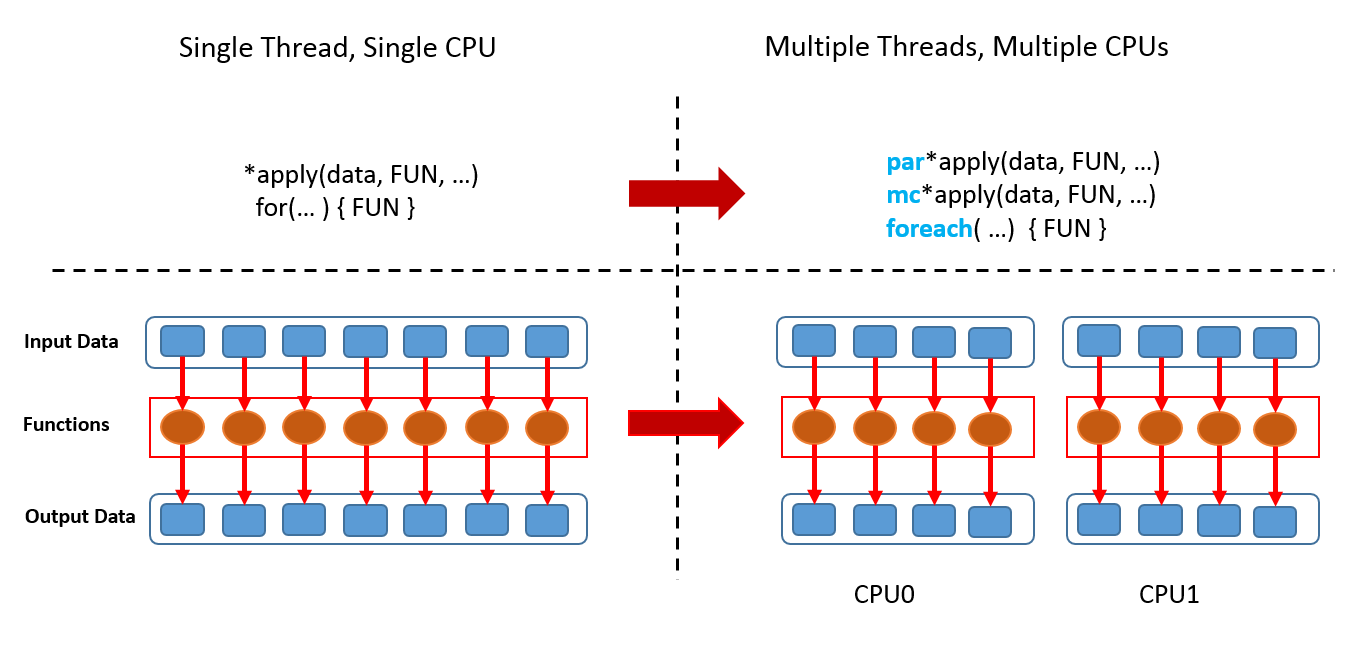
\includegraphics{images/parallel_mapping.png}
All the following runtime examinations are performed on \texttt{scrape()} which is a lightweight version of the function included in the API.
Furthermore as a general criteria for loops are avoided inside single scraping functions due to Rcpp reasons, vectorization is preferred. Through \texttt{scrape} the approach is to test two different parallel back ends performances.

The first attempt was using \texttt{furrr} package \citep{furrr} which enables mapping (i.e.~\texttt{map}) through a list from \texttt{purrr}, along with a \texttt{future} parallel back end. furrr gets along with the Tidyverse paradigm so it is expected to grow and maintained. Workers are specified though a plan with the command \texttt{plan(multisession,\ workers\ =\ 2)}. Then the function operates as many other seen purrr variations:
\texttt{furrr::future\_map(scrape(),\ .progress\ =\ T)}. Future is intuitive and easy to use, offers progress bar notifications and a dedicated website that covers also remote EC2 connections.Furthermore recently it has widened the flexibility of workers strategies by chunking strategy allowing to tweak batches of workers.
The approach has shown decent performance, but its run time drastically increases when more requests are sent. This leads to a preventive conclusion about the computational complexity: it has to be at least linear with steep slope. Empirical demonstrations have been made:

\begin{figure}
\centering
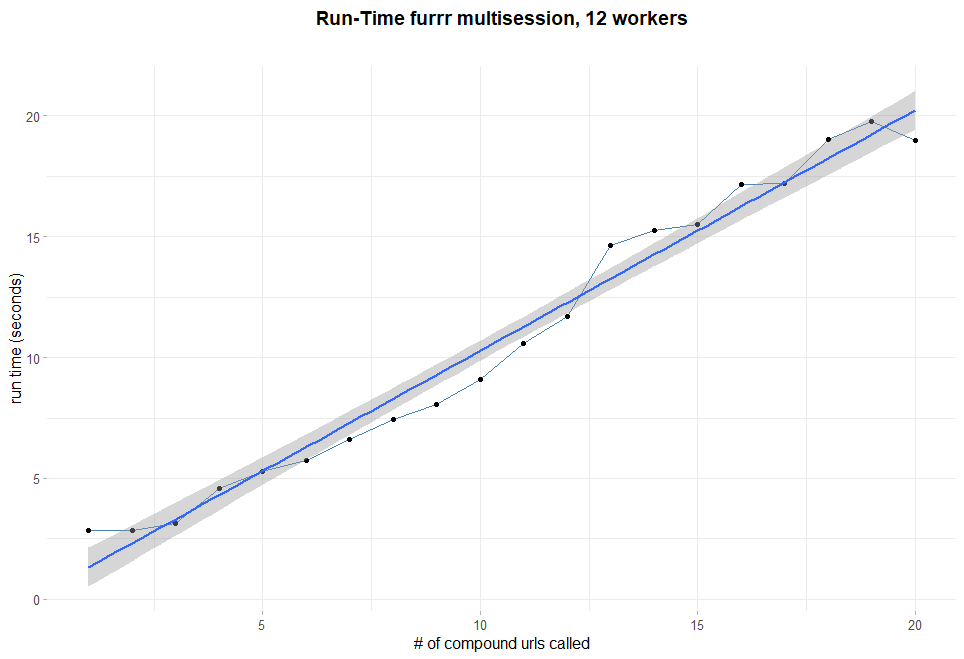
\includegraphics{images/furrr.png}
\caption{\label{fig:furrr}computational complexity analysis with Furrr}
\end{figure}

On the x-axis in the figure \ref{fig:furrr} the number of compounded urls evaluated, on y-axis the run time taken measured in seconds. Iteration after iteration the function provides to the workers 1 further link to scrape untill all the set is inputted. Looking at the blue smoothing curve in between confidence lines the big-O guess might be linear time \(\mathcal{O}(n)\), where n are the number of links considered.

A second attempt tried to explore the \texttt{foreach} package \citep{foreach} originally developed by Microsoft R. The package enables a looping construct to explicitly distribute the computations to multiple R workers. foreach does offer a vast flexibility in terms of expressing the working group and clusters of workers. foreach minimizes also operations executed by isolating the environment.

One major concern regards that functions inside the \%dopar\% should be standalone in order to be executed in parallel. For standalone it is meant that everything that is needed to be executed and to output results should be defined inside the \%dopar\%, as it would be opened a new empty environment for each iteration. Moreover as a further consequence packages imported into each clusters, the .packages methods takes care of that.

The function Flexibility comes at a cost of usability, as a matter of fact the loop constructor is much more complex with respect to furrr.
The looping construction follows the r-base looping idea, below main steps are summarized:

\begin{itemize}
\tightlist
\item
  Detect cores, initialize workers based on number of cores, register the parallel back end \texttt{registerDoParallel(cl,cores)}
\item
  define the iterator, i.e.~``i'' equal to the number of elements that are going to be looped
\item
  \texttt{.packages}: Inherits the packages that are used in the tasks define below
\item
  \texttt{.combine}: Define the combining function that bind results at the end (say cbind, rbind or tidyverse::bind\_rows).
\item
  \texttt{.errorhandling}: specifies how a task evaluation error should be handle.
\item
  \texttt{\%dopar\%}: the dopar keyword suggests foreach with parallelization method
\item
  then the function within the elements are iterated
\item
  close clusters
\end{itemize}

\begin{figure}
\centering
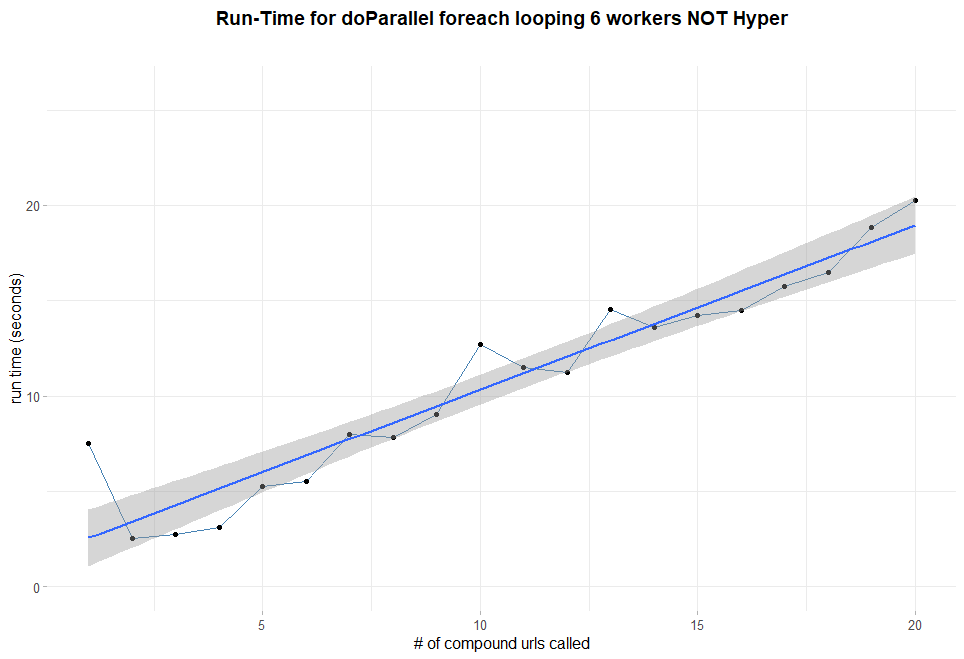
\includegraphics{images/forerach.png}
\caption{\label{fig:foreach}computational complexity analysis with Furrr}
\end{figure}

It can be grasped quite easily by figure \ref{fig:foreach} that initially foreach takes some times to set up parallel workers but then the curve is flattened and a confident guess might be .5 sloped linear time \(\mathcal{O}(\frac{n}{2})\).

\hypertarget{challenges}{%
\section{Open Challenges and Further Improvemements}\label{challenges}}

The main challenge remains unsolved since each single element has been optimized but scraping function and, as a consequence, REST API must be continuously maintained. As a matter of fact what unfortunately can not be a-priori optimized are the future changes that involves the first part of the scraping process i.e.~decomposing the website structure. Indeed Content architecture, with some further improvements can take care of finding exact information within the web page even if the design is changed. This idea is developed in the package \citet{Rcrawler}, which crawls the entire website and searches for targeted keywords, even though end results are not always acceptable. The major enhancement of this approach is that it neatly separates the website structure from the content architecture by locally saving all the html/xml files that compose the website. html are known to be very lightweight so computation of this kind is not weighing down the run time. Once all files are stored the algorithm searched for the keywords within the html, then results are grabbed. For these reasons performances with algorithm of this species are very smooth but results, as anticipated, are under the expectations. Moreover the bigger the website the slower the algorithm.
As a partial solution a more robust scraping code can be obtained integrating the existing code with accurate content text mining techniques together with unit testing integration tools like \texttt{testthat} \citet{testthat} and \texttt{usethis} \citet{usethis}. The latter packages also bring improvements during software development and ex-post a \emph{TDD} (i.e.Test-Driven Development \citet{TDD_2004}) approach would have cut API software development time. Furthermore a very popular tool to develop and automate test API is \href{https://www.postman.com/}{Postman}, which is very convenient when POST endpoints are available, since for the moment are not in existence it is not used and the default \href{https://editor.swagger.io/}{Swagger} interface takes its place.
It must be said also that \citet{Rcrawler} is designed to scrape a vast number of websites, as opposite the scraping functions here presented are exclusively built on top of immobiliare.it, even though they can be extended to other related website with no effort, for reasons pointed out in the initial part of section \ref{webstructure}.
The way this scraping functions handle errors really facilitates responsive and fast debugging but this can not be by any means neither automatized nor notified to the maintainer. The API frequently needs to be tested and to resort to CI. A better way to move toward would be integrating a CI/TD approach as said few lines ago.
On the parallel computing side further performance improvement could be obtained using a new born package called \texttt{doAzureParallel} which is built on top of the foreach. doAzureParallel enables different Virtual Machines operating parallel computing throughout Microsoft Azure cloud. This comes at a substantial monetary cost adn it is definetely not the first choice. Nonetheless it would perfectly match the need given that parallel back ends shrinks run time by accelerating the number of requests sent among different processors/cores or cluster, even though actually the goal is to differentiate sessions. Cloud Virtual Machines allow from one hand to further add computational capabilties (more processore more cores), from the other they can internalize requests among different machines (a pool of agents for each VM), extending even more the linear combination of IDs.

Moreover error messages can not sometimes be printed out in console and be undesrtood while in parallel beckend. as it is shown the \href{https://stackoverflow.com/questions/10903787/how-can-i-print-when-using-dopar}{stackoverflow reproducible example}. As a consequence to that each time an error occurs the ``main'' functions needs to be taken out of from the parallel back end and separately evaluated. This is time consuming but for the time being no solutions have been found.

\hypertarget{legal-profiles-ancora-non-validato}{%
\section{Legal Profiles (ancora non validato)}\label{legal-profiles-ancora-non-validato}}

``Data that is online and public is always available for all'' is never a good answer to the question ``Can I use those web data to my scope''. Immobiliare.it is not providing any open source data from its own database neither the perception is that it is planning to do so in the future. Immobiliare has not even provided a paid API through which data might be accessed.
A careful reading of their terms, reviewed with a intellectual property expert, has been done to get this service running without any legal consequence, as a reference the full policy can be seen in their \href{https://www.immobiliare.it/terms/}{specialized section}. Nevertheless the golden standard for scraping was respected since the robottxt is neat allowing any actions as demonstrated above. So if it might be the case of misinterpretation of their policy, it will be also the case of lack of communication between servers response and immobiliare.it intent to preserve their own intellectual property.
What it was shockingly surprising are the low barriers to obtain information with respect to other counterpart online players. Best practices are applied and delayed requests (even though not asked) have been sent to normalize traffic congestion. But scraping criteria followed are once again fully based on common shared best practises (see section \ref{best-practices}), and \emph{not} any sort of general agreements between parties. As a result a plausible approach could be applying scraping procedures without any prevention. It would not surely cause any sort of disservice for the website since budjet constraints are set low, but in the long run it will cause lagging as soon as budjet or subjects will increase. Totally different was the approach proposed by Idealista.com, which is a comparable to immobiliare.it. Idealista does block requests if they are not in compliance with their servers inner rules. User agents in this case must be rotated quite frequently and as soon as a request does not fall within the pool of user agents (i.e.~is labled as web bot) it is immediately blocked and 404 response is sent back. Delay is kindly asked and it must be specified, consequnetly this slows down scraping function per se.

\begin{itemize}
\tightlist
\item
  Idealista content is composed by Javascript so and html parser can no get that.
\item
  Idealista blocks also certain web browser that have a demonstrated ``career'' in scraping procedures.
\end{itemize}

All of this leads to accept that entry barriers to scrape are for sure higher than the one faced for Immobiliare. The reticence to share data could be a reflex on how big idealista is; as a matter of fact it has a heavy market presence in some of the Europe real estate country as Spain and France. So the hidden intention was to raise awareness on scraping procedure that in a certain remote way can hurt their business. This has been validated by the fact that prior filtering houses on their website a checkbox has to be signed. The checkbox make the user sign an agreement on their platform according to which data can not be misused and it belongs their intellectual property.

\hypertarget{Infrastructure}{%
\chapter{REST API Infrastructure}\label{Infrastructure}}

In order to provide a fast and easy to use API service to the end user many technologies have been involved. Challenges in scraping as pointed out in section \ref{challenges} are many and still some remains unsolved. Challenges regard not only scraping per se, but also the way the service has to interact with users. Interactions and subjects are many and so are obstabcles to tackle. Some of the main are:
API Service has to be executed \(n\) given times during the day at \(x-y-z\) hours and should be storing data on a cloud database, so that the evolution of the phenomenon can be monitored in time.
API service has to be fast otherwise data become obsolete and so happen to the analysis that has relied on the data.
API service has to be deployed so that it can be shared over a wider range of different background stakeholders, without having them to know what it takes. From one hand service has to be responsive to immobiliare.it unpredictable changes, thus it needs to be continuously integrated and reviewed. On the other code behind the service has to be version controlled and freezed, so that the service can guarantee continuity and prevent failures. Moreover service has to be scalable at need since, due to deployment, when the number of users increases the run time performances should not decrease. In addition API inbound traffic has to be managed both in terms traffic and security by granting access only to the ones authorized.
Open source solutions for each of the requirements are available for back-end and front-end integration. Moreover documentations related to those technologies are able to offer flexible solutions to be embedded into the R ecosystem.
Given the requirements recipe the idea is to provide a REST Plumber API with 4 endpoints each of which calls scraping functions in Parallel built in section \ref{scraping}. On top of that a daily Cron Job scheduler exposes one precise API endpoint, which produces and later stores a .csv file in a NOSQL mongoDB Atlas could database. Containerization happens through a Linux OS (Ubuntu distr) Docker container hosted by a free tier AWS EC2 server machine equipped with 30GB max capacity. API endpoints are secured with https protocols, load balanced and protected with authentication by NGINX reverse proxy server. On a second server a Shiny App calls one endpoint gievn specified parameters that returns data from the former infrastructure. A sketch of the infrastructure is represented in figure \ref{fig:CompleteStructure}.

Technologies involved are:

\begin{itemize}
\tightlist
\item
  GitHub version control
\item
  Scheduler cron job, section \ref{scheduler}
\item
  Plumber REST API, section \ref{plumberapi}
\item
  Docker containers, section \ref{docker}
\item
  NGINX reverse proxy, section \ref{nginx}
\item
  AWS (Amazon Web Services) EC2 \ref{aws}
\item
  MongoDB Atlas
\item
  Shiny
\end{itemize}

\begin{figure}
\centering
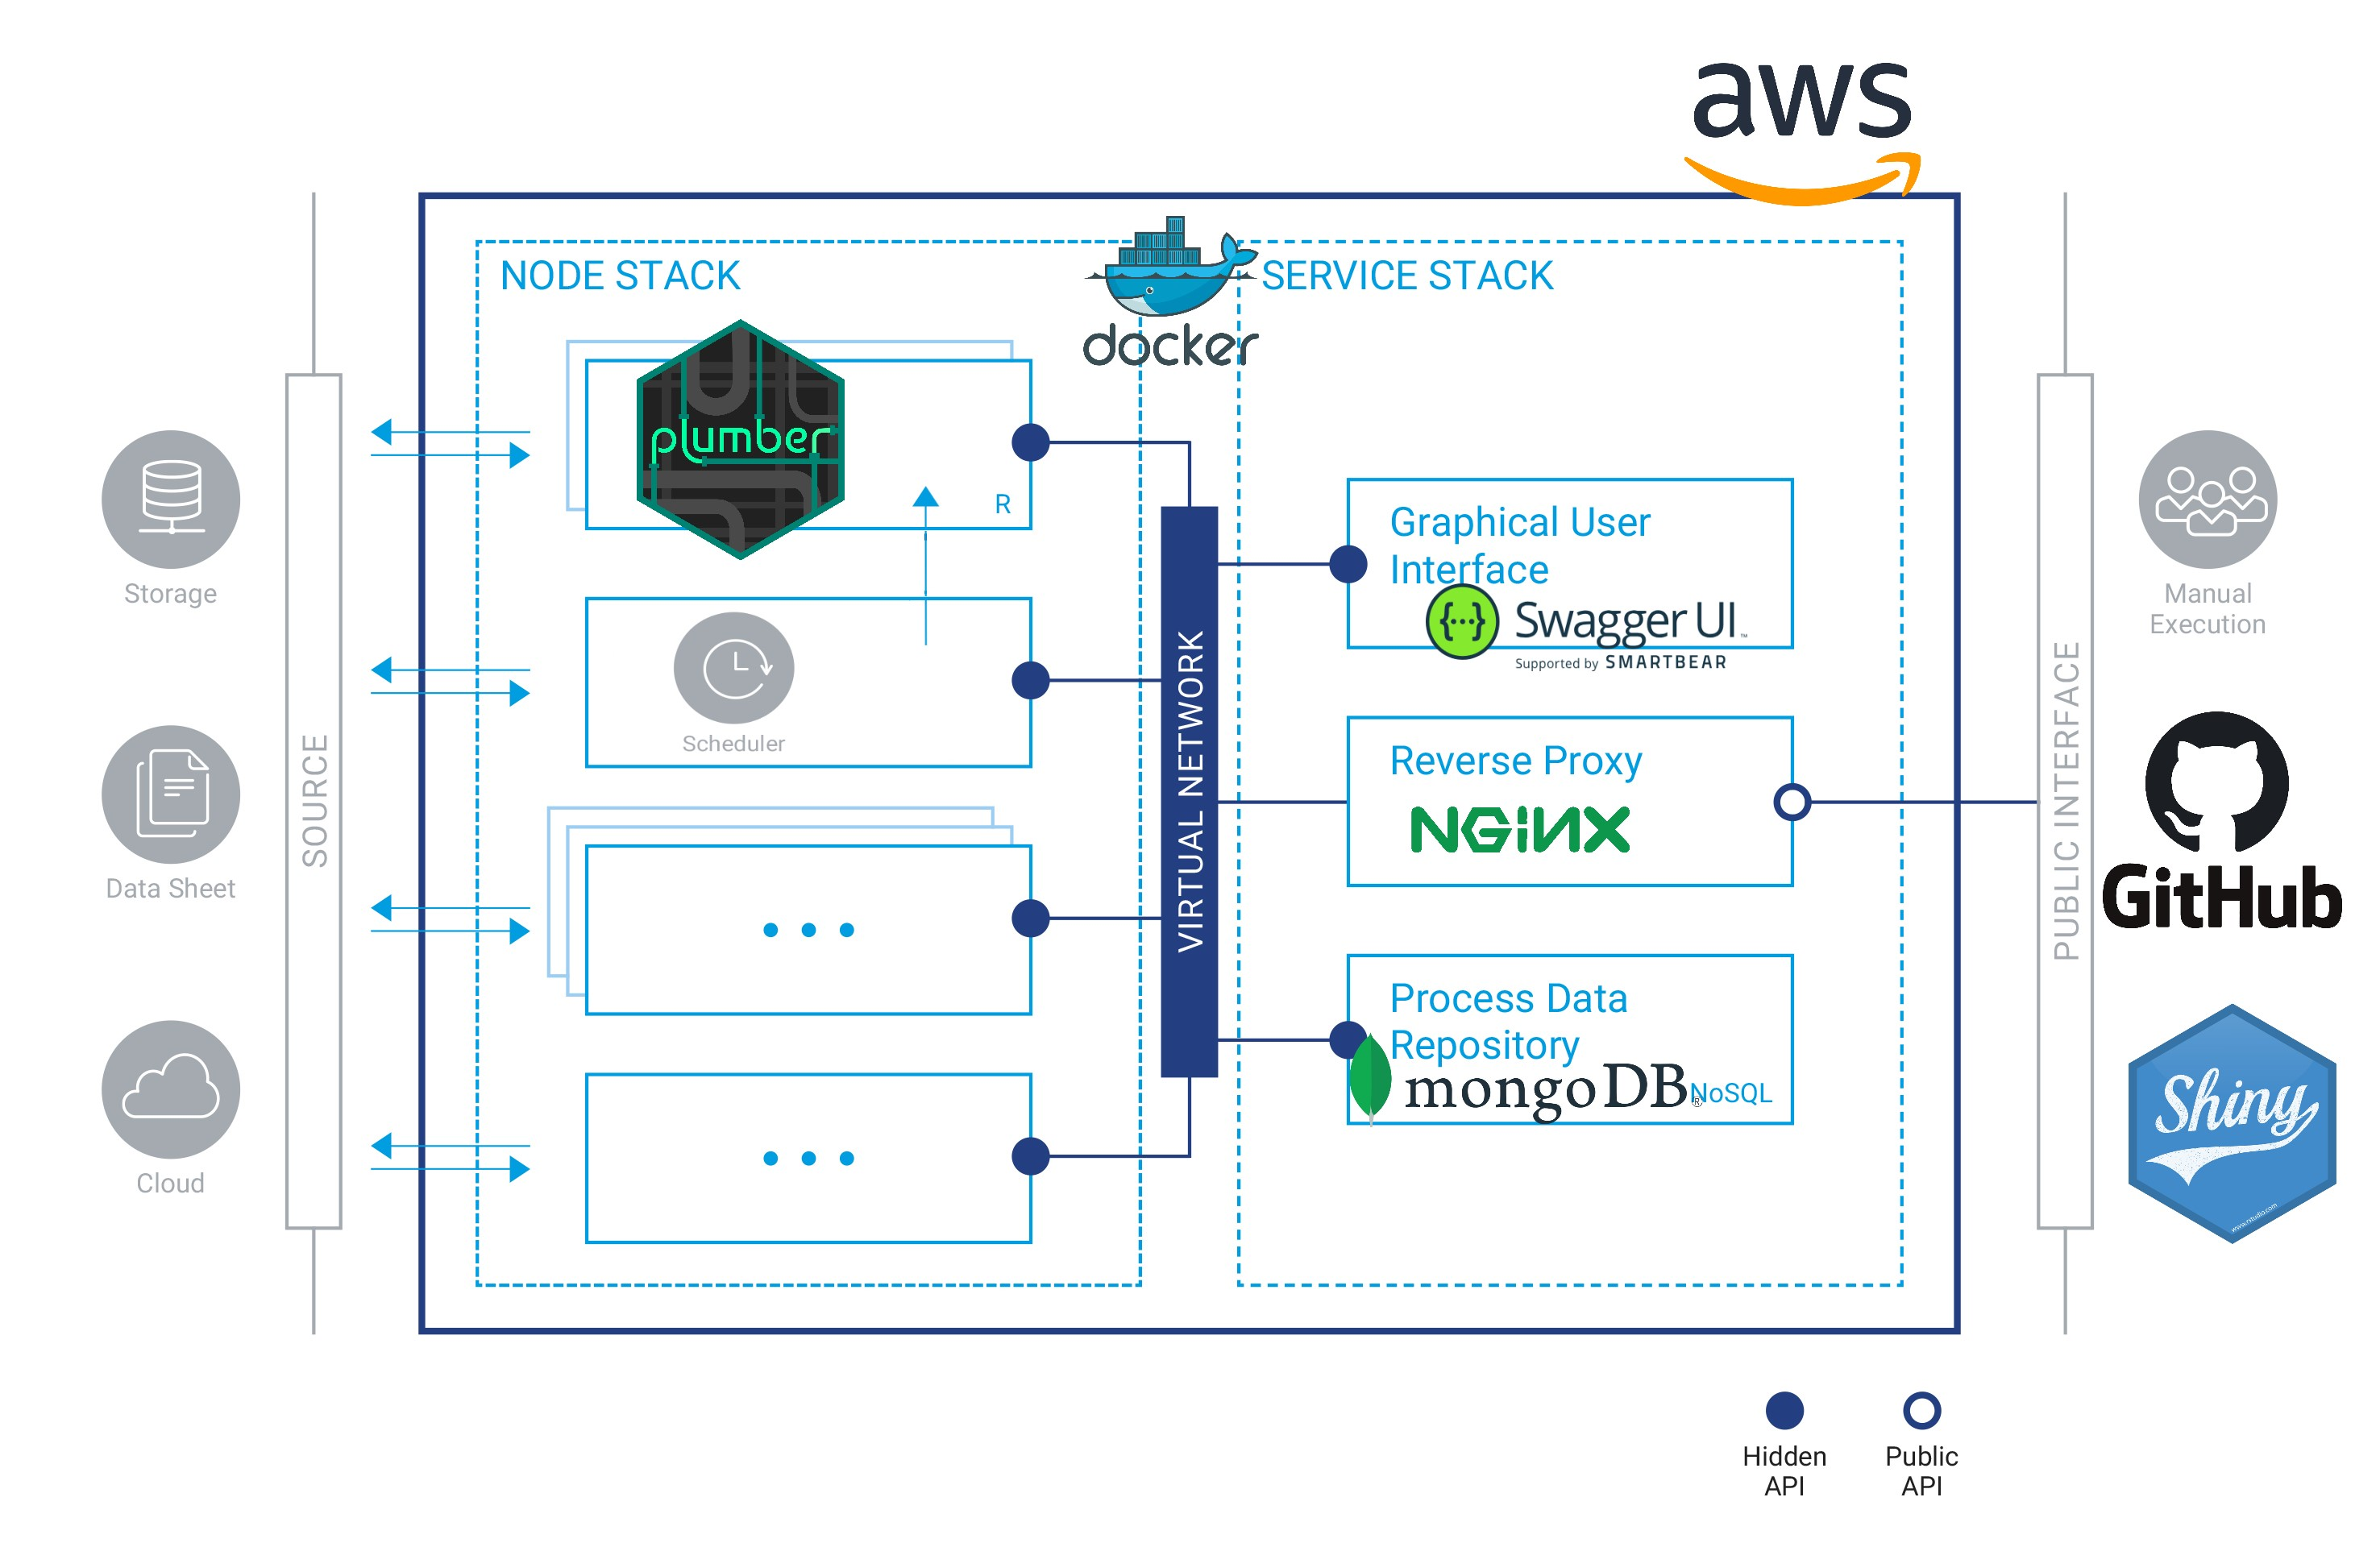
\includegraphics{images/tot_infra.jpg}
\caption{\label{fig:CompleteStructure}complete infrastructure, author's source}
\end{figure}

As a side note each single part of this thesis has been made according to some of the API inspiring criteria of sharing and self containerization. RMarkdown \citep{rmarkdown1} documents (book's chapters) are compiled and then converted into .html files. Through Bookdown \citep{bookdown2} the resulting documents are put together according to general .yml instruction file and are readble as gitbook.
Files are then pushed to a \href{https://github.com/NiccoloSalvini/thesis}{Github repository}. By a simple trick with GH pages, .html files are dispalyed into a Github subdomain hosted at \href{https://niccolosalvini.github.io/thesis/}{link}. The resulting deployed gitbook can also produce a .pdf version output through a Xelatex engine. Xelatex compiles .Rmd documents according to a .tex template which formatting rules are contained in a further .yml file. The pdf version of the thesis can be obtained by clicking the download button, then choosing pdf output version in the upper banner. For further references on the topic \citet{bookdown2}

Some of the main technologies implied will be viewed singularly, nonetheless for brevity reasons the rest needs to be skipped.

\hypertarget{scheduler}{%
\section{Scheduler}\label{scheduler}}

\begin{definition}[Scheduler]
\protect\hypertarget{def:scheduler}{}{\label{def:scheduler} \iffalse (Scheduler) \fi{} }A Scheduler in a process is a component on a OS that allows the computer to decide which activity is going to be executed. In the context of multi-programming it is thought as a tool to keep CPU occupied as much as possible.
\end{definition}

As an example it can trigger a process while some other is still waiting to finish. There are many type of scheduler and they are based on the frequency of times they are executed considering a certain closed time neighbor.

\begin{itemize}
\tightlist
\item
  Short term scheduler: it can trigger and queue the ``ready to go'' tasks

  \begin{itemize}
  \tightlist
  \item
    with pre-emption
  \item
    without pre-emption
  \end{itemize}
\end{itemize}

The ST scheduler selects the process and It gains control of the CPU by the dispatcher. In this context we can define latency as the time needed to stop a process and to start a new one.

\begin{itemize}
\tightlist
\item
  Medium term scheduler
\item
  Long term scheduler
\end{itemize}

for some other useful but beyond the scope references, such as the scheduling algorithm the reader can refer to \citep{wiki:scheduler}.

\hypertarget{cron-jobs}{%
\subsection{Cron Jobs}\label{cron-jobs}}

\begin{definition}[Cronjob]
\protect\hypertarget{def:cronjob}{}{\label{def:cronjob} \iffalse (Cronjob) \fi{} }Cron job is a software utility which acts as a time-based job scheduler in Unix-like OS. Linux users that set up and maintain software environments exploit cron to schedule their day-to-day routines to run periodically at fixed times, dates, or intervals. It typically automates system maintenance but its usage is very flexible to whichever needed. It is lightweight and it is widely used since it is a common option for Linux users.
\end{definition}
The tasks by cron are driven by a crontab file, which is a configuration file that specifies a set of commands to run periodically on a given schedule. The crontab files are stored where the lists of jobs and other instructions to the cron daemon are kept.
Each line of a crontab file represents a job, and the composition follows the syntax in figure \ref{fig:crontab}

\begin{figure}
\centering
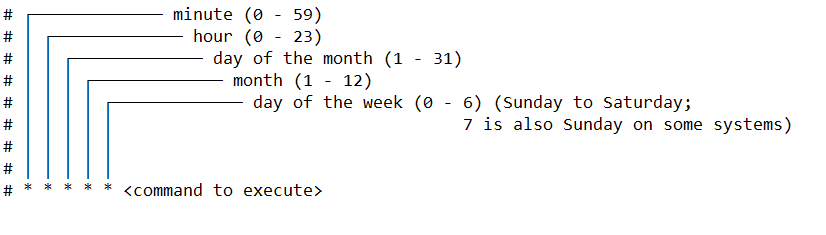
\includegraphics{images/crontab.PNG}
\caption{\label{fig:crontab}Crontab Scheduling Syntax}
\end{figure}

Each line of a crontab file represents a job. This example runs a shell named scheduler.sh at 23:45 (11:45 PM) every Saturday. .sh commands can update mails and other minor routines.

45 23 * * 6 /home/oracle/scripts/scheduler.sh

Some rather unusual scheduling definitions for crontabs can be found in this reference \citep{wiki:cronjob}. Crontab's syntax completion can be made easier through \href{https://crontab.guru/}{this} GUI.

The cron job needs to be ran on scraping fucntions at 11:30 PM every single day. The get\_data.R script first sources an endpoint function, then it applies the function with fixed parameters. Parameters describe the url specification, so that each time the scheduler runs the get\_data.R collects data from the same source. Day after day .json files are generated and then stored into a NOSQL \emph{mongoDB} database whose credentials are public. Data are collected on a daily basis with the explicit aim to track day-by-day changes both in the new entries an goners in rental market, and to investigate the evolution of price differentials over time. Spatio-Temporal modeling is still quite unexplored, data is saved for future used. Crontab configuration for daily 11:30 PM schedules has this appearance:

30 11 * * * /home/oracle/scripts/get\_data.R

To a certain extent what it has been already presented since now might fit for personal use. A scheduler can daily execute the scraping script and can generate a .csv file. Later the same .csv file can be parsed into an application and analysis can be locally reported. The solution proposed is totally \emph{not feasible} in a production environment, since in order to be executed a vast number files has to be sourced and a number of functions should be routinely called. For these reasons the present architecture can not be shared. The solution adopted tries to minimize the analyst/scientist involvement into scraping procedures by offering a compact solution that manages all the processes without having to know how scraping under the hood is working.

\hypertarget{rest-api}{%
\section{REST API}\label{rest-api}}

\begin{definition}[API]
\protect\hypertarget{def:api}{}{\label{def:api} \iffalse (API) \fi{} }API stands for application programming interface and it is a set of definitions and protocols for building and integrating application software. APIs let a product or a service communicate with other products and services without having to know how they're implemented.
\end{definition}
This can simplify app development, saving time and impacting positively on the budget due to resource savings. APIs are thought of as contracts, with documentation that represents an general agreement between parties.
There are many types of API that exploit different media and architectures to communicate with apps or services.
\begin{definition}[REST]
\protect\hypertarget{def:rest}{}{\label{def:rest} \iffalse (REST) \fi{} }The specification REST stands for REpresentational State Transfer and is a set of architectural principles.
\end{definition}
When a request is made through a REST API it transfers a representation of the state to the requester. This representation, is submitted in one out of the many available formats via HTTP: JSON (Javascript Object Notation), HTML, XLT, TXT. JSON is the most popular because it is language agnostic \citep{what_is_a_rest_api}, as well as more comfortable to be read and parsed.
In order for an API to be considered RESTful, it has to conform to these criteria:

\begin{itemize}
\tightlist
\item
  A client-server architecture made up of clients, servers, and resources, with requests managed through HTTP.
\item
  Stateless client-server communication, meaning no client information is stored between requests and each request is separate and unconnected.
\item
  Cacheable data that streamlines client-server interactions.
\item
  A uniform interface between components so that information is transferred in a standard form. This requires that:

  \begin{itemize}
  \tightlist
  \item
    resources requested are identifiable and separate from the representations sent to the client.
  \item
    resources can be manipulated by the client via the representation they receive because the representation contains enough information to do so.
  \item
    self-descriptive messages returned to the client have enough information to describe how the client should process it.
  \item
    hypermedia, meaning that after accessing a resource the client should be able to use hyperlinks to find all other currently available actions they can take.
  \end{itemize}
\item
  A layered system that organizes each type of server (those responsible for security, load-balancing, etc.) involved the retrieval of requested information into hierarchies, invisible to the client.
\end{itemize}

REST API accepts http requests as input and elaborates them through end points. An end point identifies the operation through traditional http methods (e.g.~/GET /POST) that the API caller wants to perform. Further documentation and differences between HTTP and REST API can be found to this \href{https://docs.aws.amazon.com/it_it/apigateway/latest/developerguide/http-api-vs-rest.html}{reference}.

open REST API examples:
- BigQuery API: A data platform for customers to create, manage, share and query data.
- YouTube Data API v3: The YouTube Data API v3 is an API that provides access to YouTube data, such as videos, playlists, and channels.
- Cloud Natural Language API: Provides natural language understanding technologies, such as sentiment analysis, entity recognition, entity sentiment analysis, and other text annotations, to developers.
- Skyscanner Flight Search API: The Skyscanner API lets you search for flights \& get flight prices from Skyscanner's database of prices, as well as get live quotes directly from ticketing agencies.
- Openweathermap API: current weather data for any location on Earth including over 200,000 cities.

\begin{figure}
\centering
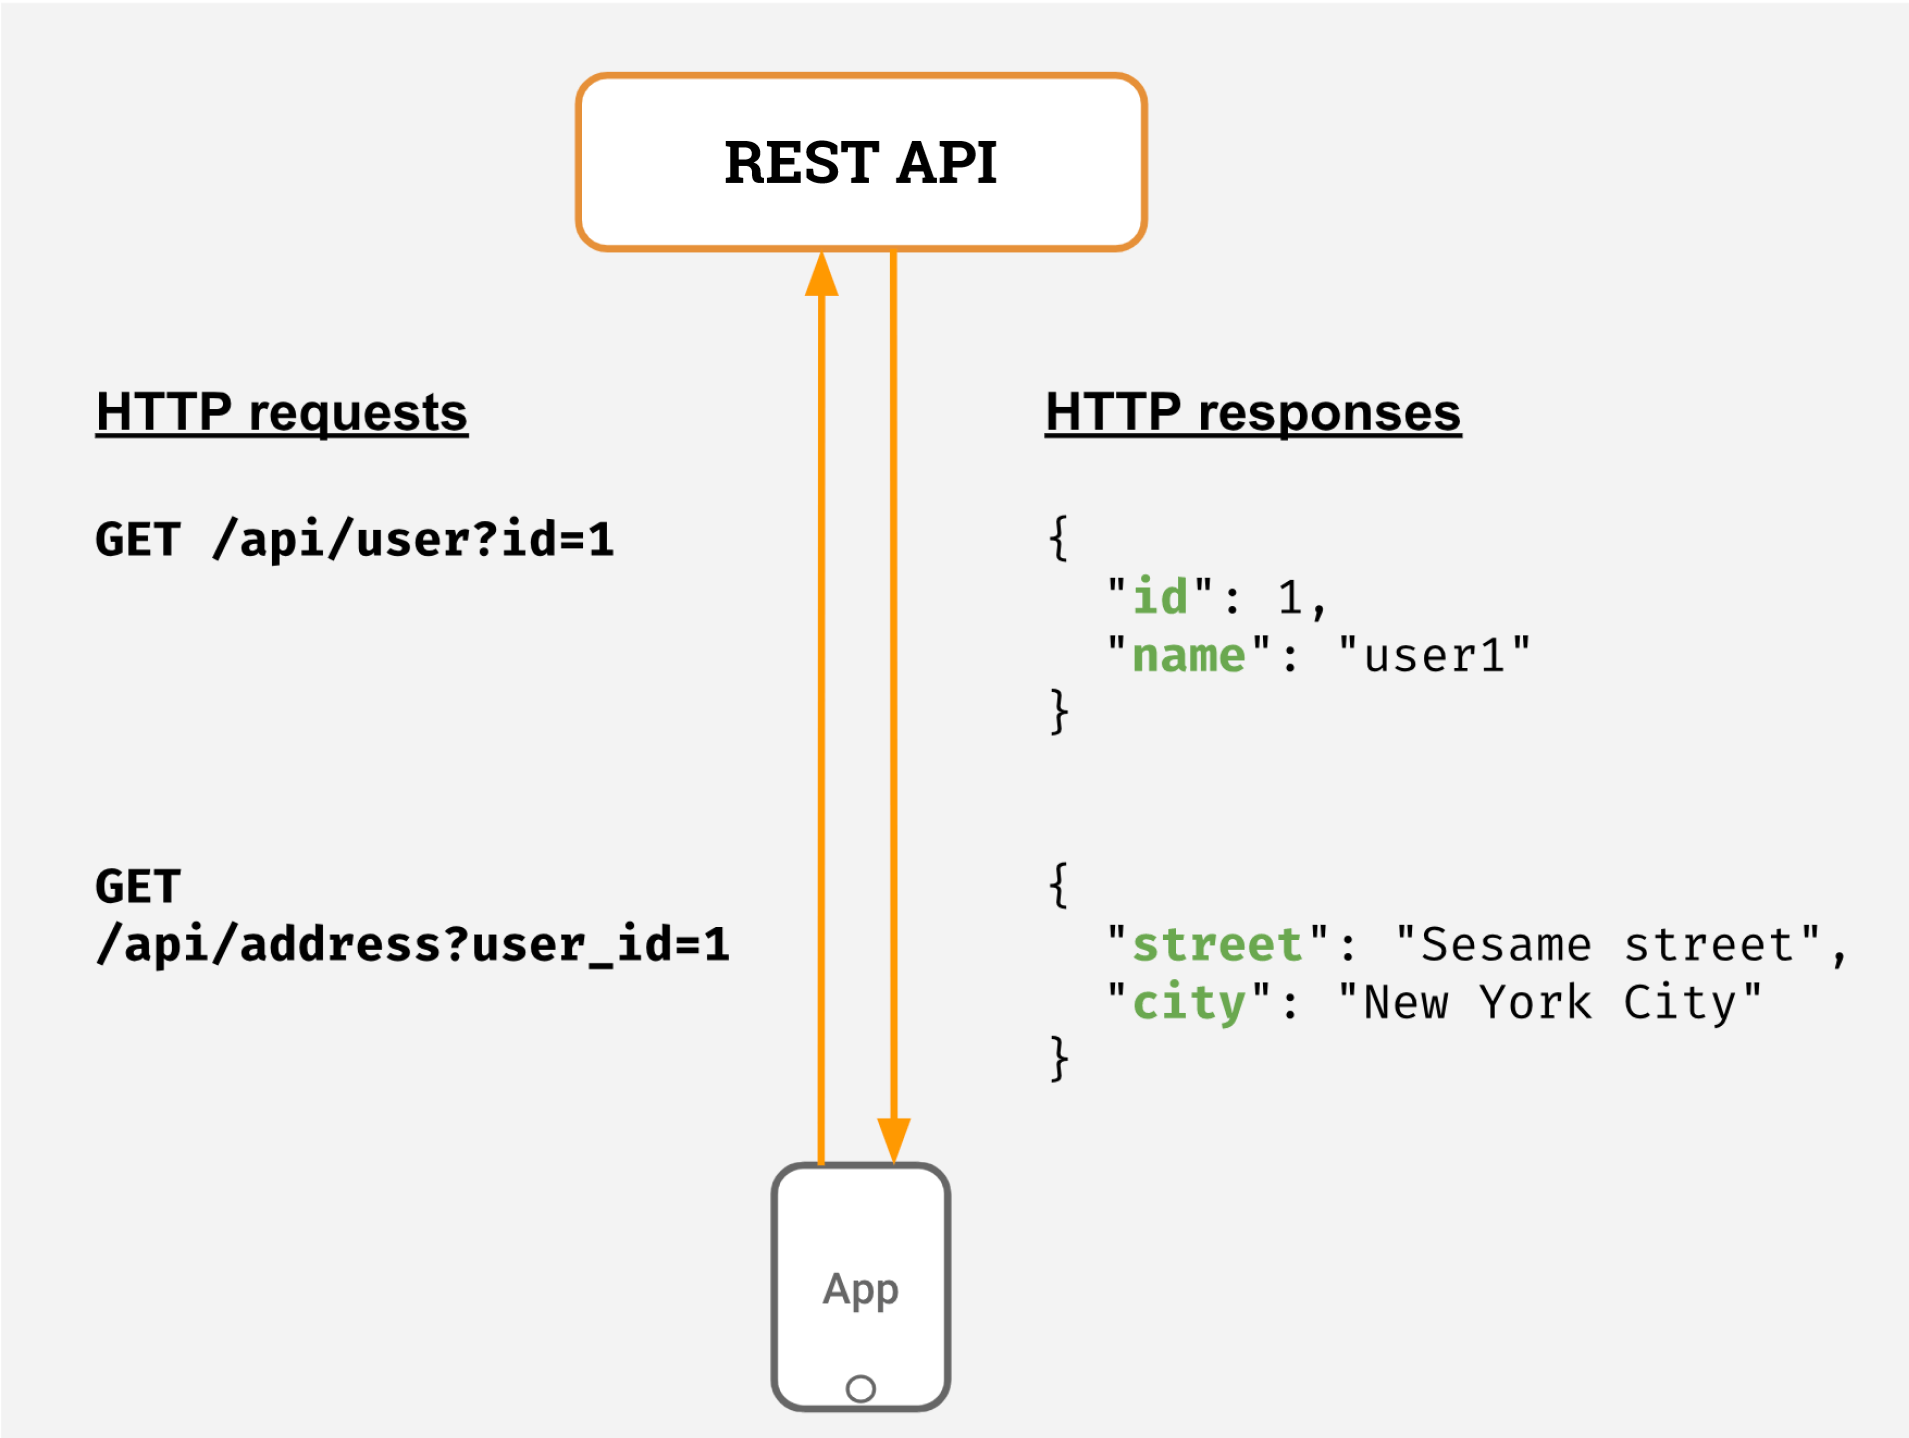
\includegraphics{images/Rest-API.png}
\caption{API general functioning functioning}
\end{figure}

\hypertarget{plumberapi}{%
\subsection{Plumber REST API}\label{plumberapi}}

Plumber allows the user to create a REST API by adding decoration comments to the existing R code, in this case to scraping code. Decorations are a special type of comments that suggests to Plumber where and when the API specifications parts are. Below a simple example extracted by the documentation:

\begin{Shaded}
\begin{Highlighting}[]
\CommentTok{# plumber.R}

\CommentTok{#* Echo back the input}
\CommentTok{#* @param msg The message to echo}
\CommentTok{#* @get /echo}
\ControlFlowTok{function}\NormalTok{(}\DataTypeTok{msg=}\StringTok{""}\NormalTok{) \{}
  \KeywordTok{list}\NormalTok{(}\DataTypeTok{msg =} \KeywordTok{paste0}\NormalTok{(}\StringTok{"The message is: '"}\NormalTok{, msg, }\StringTok{"'"}\NormalTok{))}
\NormalTok{\}}

\CommentTok{#* Plot a histogram}
\CommentTok{#* @serializer png}
\CommentTok{#* @get /plot}
\ControlFlowTok{function}\NormalTok{() \{}
\NormalTok{  rand =}\StringTok{ }\KeywordTok{rnorm}\NormalTok{(}\DecValTok{100}\NormalTok{)}
  \KeywordTok{hist}\NormalTok{(rand)}
\NormalTok{\}}

\CommentTok{#* Return the sum of two numbers}
\CommentTok{#* @param a The first number to add}
\CommentTok{#* @param b The second number to add}
\CommentTok{#* @post /sum}
\ControlFlowTok{function}\NormalTok{(a, b) \{}
  \KeywordTok{as.numeric}\NormalTok{(a) }\OperatorTok{+}\StringTok{ }\KeywordTok{as.numeric}\NormalTok{(b)}
\NormalTok{\}}
\end{Highlighting}
\end{Shaded}

three endpoints associated to 2 /GET and 1 /POST requests are made available. Functions are made clear without names so that whenever the endpoint is called functions are directly executed.
Decorations are marked as this \texttt{\#*} and they are followed by specific keywords denoted with \texttt{@}.
- the \texttt{@params} keyword refers to parameter that specifies the corpus of the HTTP request, i.e.~the inputs with respect to the expected output. If default parameters are inputted then the API response is the elaboration of the functions with default parameters. As opposite endpoint function elaborates the provided parameters and returns a response.
- \texttt{\#*\ @serializer} specifies the extension of the output file when needed.
- \texttt{\#*\ @get} specifies the method of HTTP request sent.
- \texttt{/echo} is the end point name.
- \texttt{@filter} decorations activates a filter layer which are used to track logs and to parse request before passing the argbody to the end points.

Many more options are available to customize plumber API but are beyond the scope, a valuable resource for further insights can be found in the dedicated package website \citep{an_api_generator_for_r}

\hypertarget{immobiliare.it-rest-api}{%
\subsection{Immobiliare.it REST API}\label{immobiliare.it-rest-api}}

The API service is composed by 4 endpoints \emph{/scrape} , \emph{/links}, \emph{/complete} and \emph{/get\_data}:

\begin{itemize}
\item
  */scrape performs a fast scraping of the website that leverages a rooted tree shortest path to get to data. This comes at the cost of the number of available covariates to scrape which are 5: title, price, number of rooms, sqmeter, primarykey. By default the end point scrape data from Milan real estate rents. It is a superficial and does not contain geospatial, however it might fit for some basic regression settings. The macrozone parameter allows to specify the NIL (Nucleo Identità Locale), targeting very detailed zones in some of the cities for which is available (Roma, Firenze, Milano, Torino).
\item
  */links: extracts the list of each single advertisement link belonging to each of the npages parameter specified, reacall section \ref{webstructure}. It displays sufficient performances in terms of run time. It is strictly needed to apply the following endpoint. .thesis options secures a pre combined url with the data wanted for thesis analysis. The option takes care to decompose the website structure of the url supplied with the aim to apply scraping function in the /complete endopoint.
\item
  */complete: both the function all.links and complete are sourced. The former with the aim to grab each single links and store it into an object. The latter to actually iterate scraping on each of the links.
\item
  */get\_data: it triggers the data extraction by sourcing the /complete endpoint and then storing .json file into the NOSQL mongoDB ATLAS
\end{itemize}

\begin{figure}
\centering
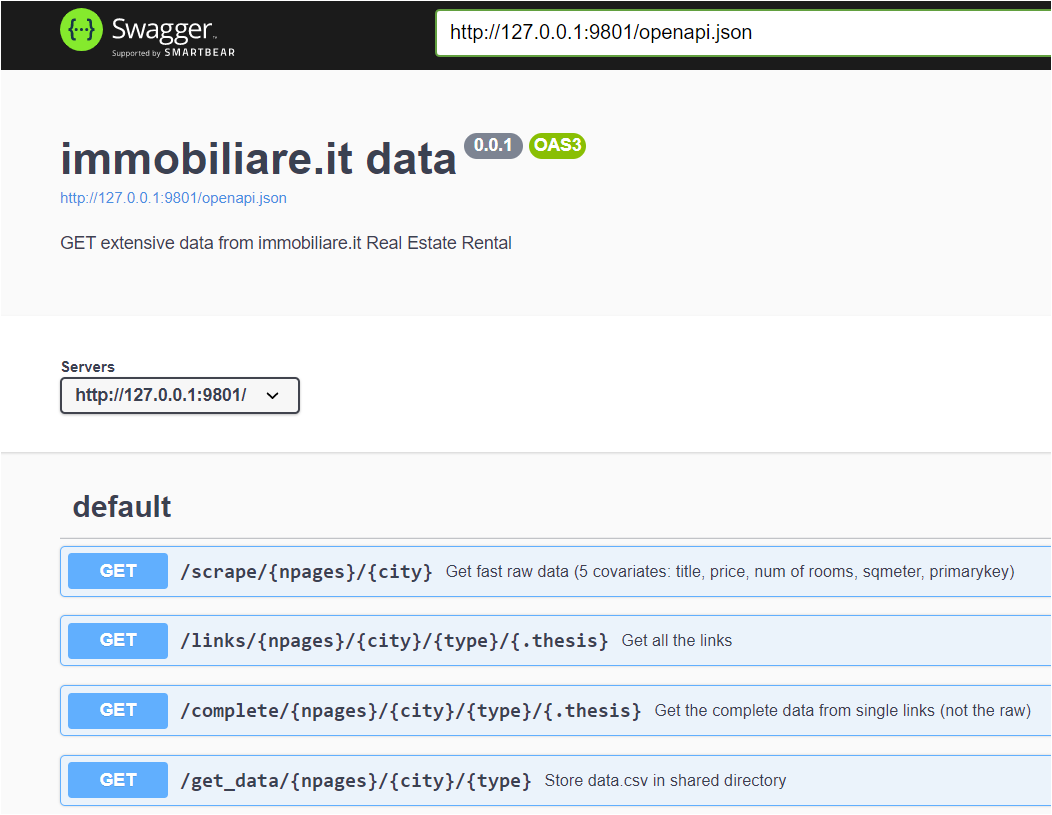
\includegraphics{images/swagger.PNG}
\caption{Swagger UI screenshot, author's source}
\end{figure}

\hypertarget{APIdocs}{%
\subsection{REST API documentation}\label{APIdocs}}

\begin{itemize}
\tightlist
\item
  Get FAST data, it covers 5 covariates:
\end{itemize}

\begin{verbatim}
      GET */scrape
      @param city [chr string] the city you are interested in (e.g. "roma", "milano", "firenze"--> lowercase, without accent)
      @param npages [positive integer] number of pages to scrape, default = 10, min  = 2, max = 300
      @param type [chr string] "affitto" = rents, "vendita"  = sell 
      @param macrozone [chr string] avail: Roma, Firenze, Milano, Torino; e.g. "fiera", "centro", "bellariva", "parioli" 
      content-type: application/json 
\end{verbatim}

\begin{itemize}
\tightlist
\item
  Get all the links
\end{itemize}

\begin{verbatim}
      GET */link
      @param city [chr string] the city you are interested to extract data (lowercase without accent)
      @param npages [positive integer] number of pages to scrape default = 10, min  = 2, max = 300
      @param type [chr string] "affitto" = rents, "vendita"  = sell 
      @param .thesis [logical] data used for master thesis
      content-type: application/json 
\end{verbatim}

\begin{itemize}
\tightlist
\item
  Get the complete set of covariates (52) from each single links, takes a while
\end{itemize}

\begin{verbatim}
      GET */complete
      @param city [chr string] the city you are interested to extract data (lowercase without accent)
      @param npages [positive integer] number of pages to scrape default = 10, min  = 2, max = 300
      @param type [chr string] "affitto" = rents, "vendita"  = sell 
      @param .thesis [logical] data used for master thesis
      content-type: application/json
\end{verbatim}

Up to this point the API can smoothly run in local and potentially can be deployed to share results without requesting scraping process knowledge. However the API software for now is not portable and is very heavy. In addition it can also run into failures for many reasons, one among the others is package versione incompatibility due to updates. In the end it also fully relies on the laptop computational power that can be heavily stressed when a number of API calls are executed, especially for single threaded programming languages as R.
The approach followed proposes a dedicated lightweight software environment that minimizes dependencies both improving performances and enabling the \emph{cloud computing} coverage. A fast growing techonlogy is what fits the need.

\hypertarget{docker}{%
\section{Docker}\label{docker}}

\begin{definition}[Docker]
\protect\hypertarget{def:docker}{}{\label{def:docker} \iffalse (Docker) \fi{} }\emph{Docker} is a software tool to create and deploy applications using containers.
\emph{Docker containers} are a standard unit of software (i.e.~software boxes) where everything needed for applications, such as libraries or dependencies can be run reliably and quickly. Furthermore they are also portable, in the sense that they can be taken from one computing environment to the following. Docker containers by default run on kernel Linux OS.
\end{definition}
Containers can be thought as an abstraction at the app layers that groups code and dependencies together. One major advantage of containers is that multiple containers can run on the same machine with the same OS. Each container can run its own isolated process in the user space, so that each task is complementary to the other. Containers are lightweight and take up less space than Virtual Machines (container images are files which can take up typically tens of MBs in size), can handle more applications and require fewer Virtual Machines and OS. The structure differences are figrued in @ref(fig:\label{fig:dockervsvm}).

\begin{figure}
\centering
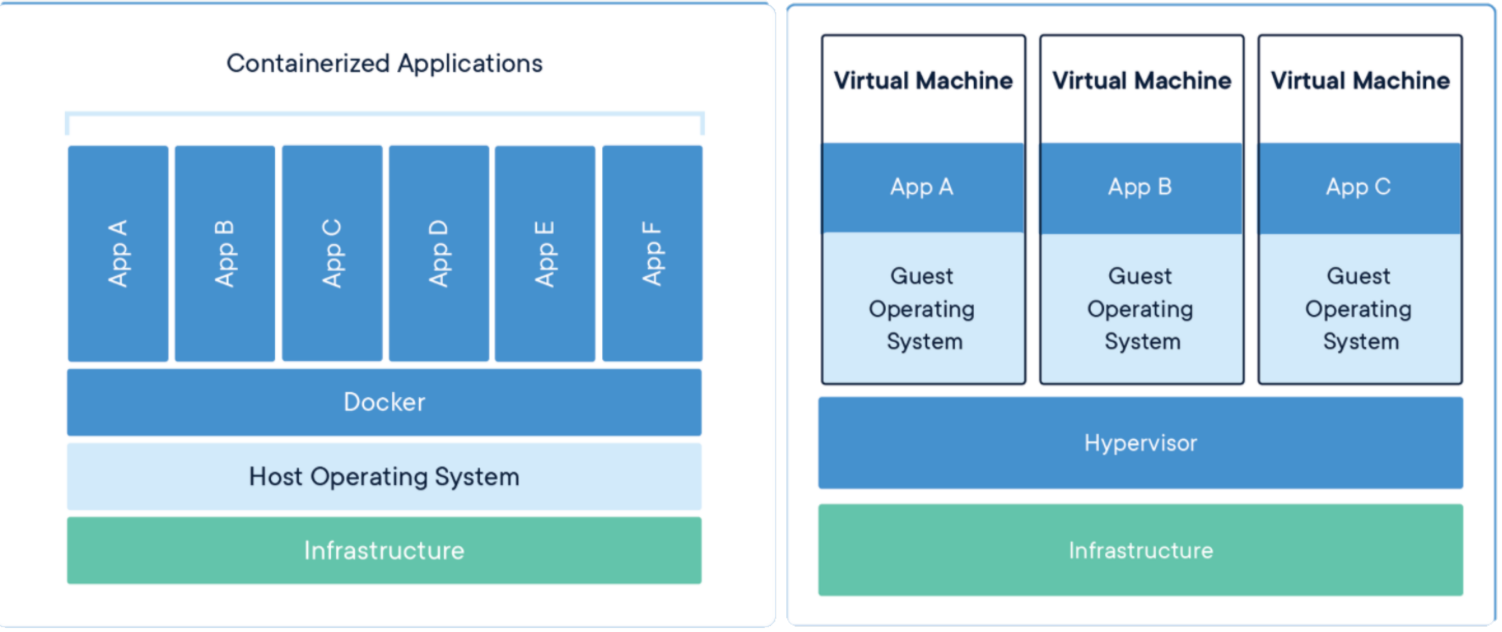
\includegraphics{images/dockerVSvirtualmachines.PNG}
\caption{\label{fig:dockervsvm}Docker containers versus Virtual Machines, \emph{miss source}}
\end{figure}

When containers are built \emph{Docker container Images} are created and can be open sourced through Docker Hub.
\emph{Docker Hub} is a web service provided by Docker for searching and sharing container images with other teams or developers in the community. Docker Hub can connect with GitHub behind authorization entailing an image version control tool. Once the connection is established changes that are pushed with git to the GitHub repository are passed to Docker Hub. The push command automatically triggers the image building. Then docker image can be tagged (salvini/api-immobiliare:latest)so that on one hand it is recognizable and on the other can be reused in the future. Once the building stage is completed the DH repository can be pulled and then run locally on machine or cloud, see section \ref{aws}.
Docker building and testing images can be very time consuming. R packages can take a long time to install because code has to be compiled, especially if using R on a Linux server or in a Docker container.
Rstudio \href{https://packagemanager.rstudio.com/client/\#/}{package manager} includes beta support for pre-compiled R packages that can be installed faster. This dramatically reduces packages time installation \citep{nolis_2020}.
In addition to that an open source project \href{https://www.rocker-project.org/images/}{rocker} has narrowed the path for developers by building custom R docker images for a wide range of usages. What can be read from their own website about the project is: ``The rocker project provides a collection of containers suited for different needs. find a base image to extend or images with popular software and optimized libraries pre-installed. Get the latest version or a reproducible fixed environment''.

\hypertarget{why-docker}{%
\subsection{Why Docker}\label{why-docker}}

\href{https://it.indeed.com/}{Indeed}, an employment-related search engine, released an article on 2019 displaying changing trends from 2015 to 2019 in Technology Job market, a summary of those changes is in figure \ref{fig:indeedstats}. Many changes are relevant in key technologies. Two among the others technologies (i.e.~docker and Azure, arrow pointed) have experienced a huge growth and both refer to the certain demand input: \emph{containers} and \emph{cloud computing}.
The landscape of Data Science is changing from reporting to application building:
In 2015 - Businesses reports drive better decisions.
In 2020 - Businesses need apps to empower better decision making at all levels.

\begin{figure}
\centering
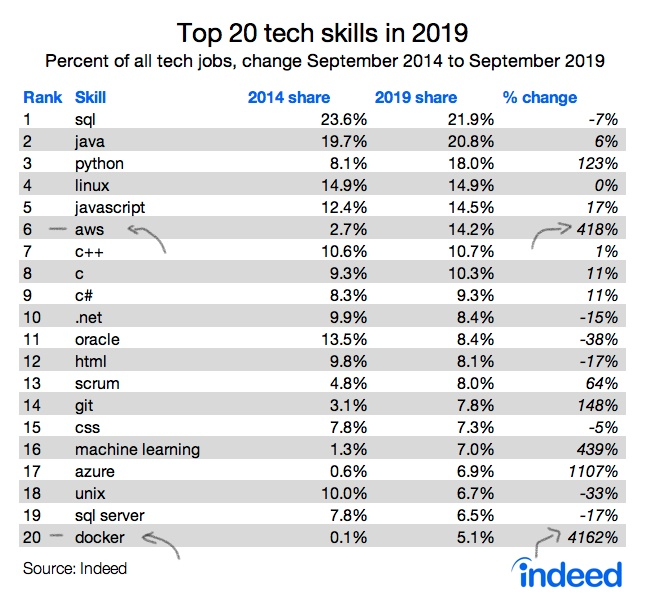
\includegraphics{images/Inkedindeed_jobs_LI.jpg}
\caption{\label{fig:indeedstats}Indeed top skills for 2019 in percent changes, \citet{top_tech_skills} source}
\end{figure}

For all the things said what docker is bringing to business are \citep{red_hat_customer_portal}:

\begin{itemize}
\tightlist
\item
  \emph{Speed application deployment} : containers include the minimal run time requirements of the application, reducing their size and allowing them to be deployed quickly.
\item
  \emph{Portability across machines} : an application and all its dependencies can be bundled into a single container that is independent from the host version of Linux kernel, platform distribution, or deployment model. This container can be transferred to another machine that runs Docker, and executed there without compatibility issues.
\item
  \emph{Version control and component reuse} : you can track successive versions of a container, inspect differences, or roll-back to previous versions. Containers reuse components from the preceding layers, which makes them noticeably lightweight. In addition due to Docker Hub it is possible to establish a connection between Git and DockerHub. Vesion
\item
  \emph{Sharing} : you can use a remote repository to share your container with others. It is also possible to configure a private repository hosted on Docker Hub.
\item
  \emph{Lightweight footprint and minimal overhead} : Docker images are typically very small, which facilitates rapid delivery and reduces the time to deploy new application containers.
\item
  \emph{Fault isolation} :Docker reduces effort and risk of problems with application dependencies. Docker also freezes the environment to the preferred packages version so that it guarantees continuity in deployment and isolate the container from system fails coming from package version updates.
\end{itemize}

The way to tell docker which system requirements are needed in the newly born software is a \emph{Dockerfile}.

\hypertarget{dockerfile}{%
\subsection{Dockerfile}\label{dockerfile}}

Docker can build images automatically by reading instructions from a Dockerfile. A Dockerfile is a text document that contains all the commands/rules a generic user could call on the CLI to assemble an image. Executing the command \texttt{docker\ build} from shell the user can trigger the image building. That executes sequentially several command-line instructions. For thesis purposes a Dockerfile is written with the specific instructions and then the file is pushed to GitHub repository. Once pushed DockerHub automatically parses the repository looking for a plain text file whose name is ``Dockerfile''. When It is matched then it triggers the building of the image.

The Dockerfile used to trigger the building of the docker container has the following sequential set of instructions in figure \ref{fig:dockerfile}) :

\begin{figure}
\centering
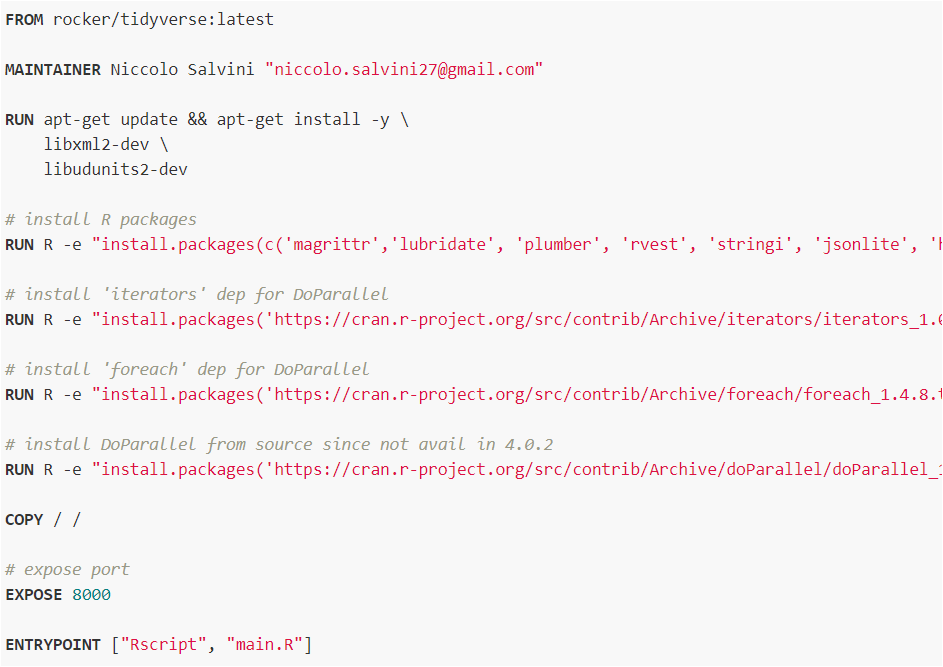
\includegraphics{images/dockerfile.PNG}
\caption{\label{fig:dockerfile}Example of a Dockerfile from Docker Hub, author's source}
\end{figure}

where the instructions are:

\begin{itemize}
\item
  \texttt{FROM\ rocker/tidyverse:latest} : The command imports a pre-built image by the rocker team that contains the latest (tag latest) version of base-R along with the tidyverse packages.
\item
  \texttt{MAINTAINER\ Niccolo\ Salvini\ "niccolo.salvini27@gmail.com"} : The command tags the maintainer and its e-mail contact information.
\item
  \texttt{RUN\ apt-get\ update\ \&\&\ apt-get\ install\ -y\ \textbackslash{}\ libxml2-dev\ \textbackslash{}\ libudunits2-dev} :The command update and install Linux dependencies needed for running R packages. \texttt{rvest} requires libxml2-dev and \texttt{magrittr} needs libudunits2-dev. If they are not installed then associated libraries can not be loaded. Linux dependencies needed have been found by trial and error while building containers. Building logs messages print errors and suggest which dependency is mandatory.
\item
  \texttt{RUN\ R\ -e\ "install.packages(c(\textquotesingle{}plumber\textquotesingle{},\textquotesingle{}tibble\textquotesingle{},\textquotesingle{}...\textquotesingle{},dependencies=TRUE)} : the command install all the packages required to execute the files (R files) containerized for the scraping. Since all the packages have their direct R dependencies the option \texttt{dependencies=TRUE} is needed.
\item
  \texttt{RUN\ R\ -e\ "install.packages(\textquotesingle{}https://cran.r-project.org/.../iterators,\ type=\textquotesingle{}source\textquotesingle{})}
  \texttt{RUN\ R\ -e\ "install.packages(\textquotesingle{}https://cran.r-project.org/.../foreach/,\ type=\textquotesingle{}source\textquotesingle{})}
  \texttt{RUN\ R\ -e\ "install.packages(\textquotesingle{}https://cran.r-project.org/.../doParallel,\ type=\textquotesingle{}source\textquotesingle{})}
  DoParallel was not available in package manager for R version later than 4.0.0. For this reason the choice was to install a previous source version by the online repository, as well as its dependencies.
\item
  \texttt{COPY\ \textbackslash{}\textbackslash{}} The command tells Docker copies all the files in the container.
\item
  \texttt{EXPOSE\ 8000} : the commands instructs Docker that the container listens on the specified network ports 8000 at runtime. It is possible to specify whether the port exposed listens on UDP or TCP, the default is TCP (this part needs a previous set up previous installing, for further online documentation It is recommended \citep{docker_documentation_2020} )
\item
  \texttt{ENTRYPOINT\ {[}"Rscript",\ "main.R"{]}} : the command tells docker to execute the file main.R within the container that triggers the API start. In main.R it are pecified both the port and the host where API expects to be exposed (in this case port 8000).
\end{itemize}

In order to make the system stand-alone and make the service available to a wider range of subjects a choice has to be made. The service has to have both the characteristics to be run on demand and to specify query parameters.

\hypertarget{nginx}{%
\section{NGINX reverse proxy server}\label{nginx}}

For analysis purposes NGINX is open source software for reverse proxying and load balancing.
Proxying is typically used to distribute the load among several servers, seamlessly show content from different websites, or pass requests for processing to application servers over protocols other than HTTP.
{[}\ldots{]}

When NGINX proxies a request, it sends the request to a specified proxied server, fetches the response, and sends it back to the client. It is possible to proxy requests to an HTTP server (another NGINX server or any other server) or a non-HTTP server (which can run an application developed with a specific framework, such as PHP or Python) using a specified protocol. Supported protocols include FastCGI, uwsgi, SCGI, and memcached.
{[}\ldots{]}

.conf file and installation on Linux server. Security and Authentication.

\hypertarget{aws}{%
\section{AWS EC2 server}\label{aws}}

Executing REST API on a public server allows to share data with a various number of services thorugh multitude of subjects. Since it can not be specified a-priori how many times and users are going to enjoy the service a scalable solutio might fill the needs. Scalable infrastructure through a flexible cloud provider combined with nginx load balancing can offer a stable and reliable infrastructure for a relatively cheap price.
AWS offers a wide range of services each of which for a wide range of budgets and integration. Free tier servers can be rent up to a certain amount of storage and computation that nearly 0s the total bill. The cloud provider also has a dedicated webpage to configure the service needed with respect to the usage named \href{https://aws.amazon.com/en/aws-cost-management/}{amazon cost manager}.

\begin{definition}[AWS EC2]
\protect\hypertarget{def:aws}{}{\label{def:aws} \iffalse (AWS EC2) \fi{} }Amazon Elastic Compute Cloud (EC2) is a web service that contributes to a secure, flexible computing capacity in the AWS cloud. EC2 allows to rent as many virtual servers as needed with customized capacity, security and storage.
\end{definition}

{[}few words still on EC2{]}

\hypertarget{launch-an-ec2-instance}{%
\subsection{Launch an EC2 instance}\label{launch-an-ec2-instance}}

The preliminary step is to pick up an AMI (Amazon Machine Image). AWS AMI are already-set-up machines with stadardized specification designed to speed up the process of choosing the a customed machine. Since the project is planned to be nearly 0-cost a ``Free Tier Eligible'' server is chosen. By checking the Free Tier box all the available free tiers are displayed. The machine selected has this specification: t2.micro with 1 CPU and 1GB RAM and runs on a Ubuntu distribution OS. First set up settings needs to be left as-is, networking and VPC can always be updated when needed. In the ``add storage'' step 30 GB storage are selected, moreover 30 represent the upper limit since the server can be considered free tier. Tags windows are beyond the scope. Secondly configuration needs to account security and a new entry below SSH connection (port 22) has to be set in. New security configuration has to have TCP specification and should be associated to port 8000. Port 8000, as in dockerfile section \ref{dockerfile}, has been exposed and needs to be linked to the security port opened.

\begin{figure}
\centering
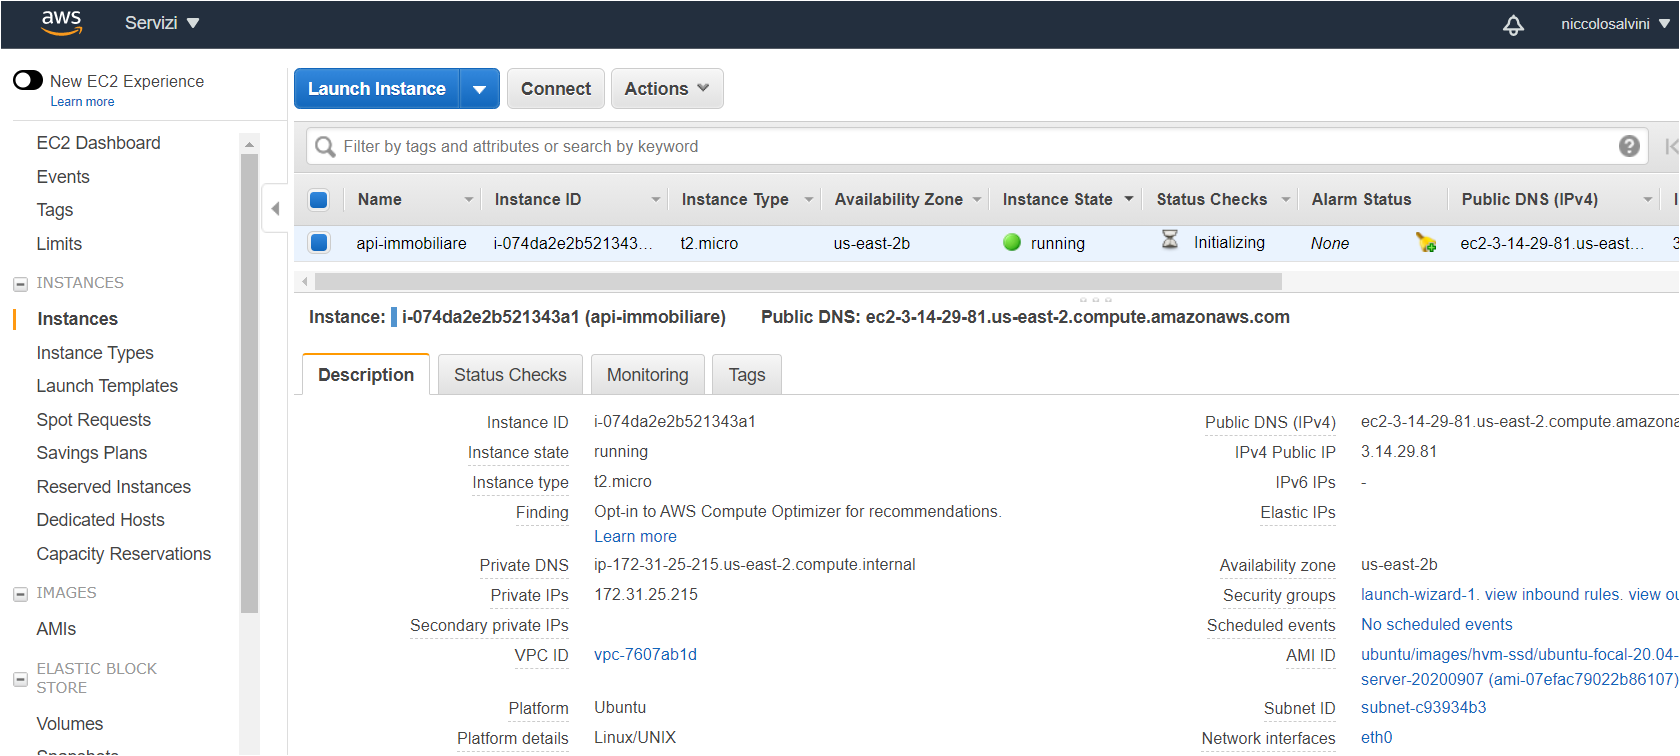
\includegraphics{images/aws.PNG}
\caption{aws\_dashboard}
\end{figure}

At this point instance is prepared to run and in a few minutes is deployed. Key pairs, if never done before, are generated and a .pem file is saved and securely stored. Key pairs are a mandatory step to log into the Ubuntu server via SSH. SSH connection in Windows OS can be handled with \href{https://www.putty.org/}{PuTTY}, which is a SSH and telnet client designed for Windows. At first PuTTYgen, a PuTTY extensions, has to convert the key pair .pem file into a .ppk extension (otherwise PuTTY can not read it). Once .ppk is converted is immediately sourced in the authorization panel. If everything works and authentication is verified then the Ubuntu server CLI appears and interaction with the server is made possible.
Once the CLI pops out some Linux libraries to check file structure (``tree'') and Docker are installed. Then a connection with Docker hub is established providing user login credentials. From the Hub repository the container image is pulled on the machine and is then executed with the docker RUN command.
AWS automatically assign to the server a unique Public DNS address which is going to be the REST API url to call.
the Public DNS has the following form:ì

\texttt{ec2-18-224-40-67.us-east-2.compute.amazonaws.com}

\hypertarget{further-integrations}{%
\section{Further Integrations}\label{further-integrations}}

Pins is an r packages \href{https://rstudio.com/resources/rstudioconf-2020/deploying-end-to-end-data-science-with-shiny-plumber-and-pins/?mkt_tok=eyJpIjoiTmprNU1USXhPVEprWXpNMSIsInQiOiJtTUhKVzlvSjVIV2hKc0NRNVU1NTRQYSsrRGd5MWMyemlTazQ5b1lHRGJXNVBLcnpScjZRaWVcL2JGUjBPNGIwV3pwY1dKTW45cnhcL2JzZUlGWndtSFNJZVNaOUcyc1ZXcEJOcnppSVJXSGZRSVU1ZUY1YUU2NWdDamoxZG5VMHZcLyJ9}{this link}
software development framework and tools for testing \href{https://github.com/isteves/plumbplumb}{this work}

\hypertarget{inla}{%
\chapter{INLA computation}\label{inla}}

INLA \citep{Rue2009} stands for Integrated Nested Laplace approximation and constitutes a computational alternative to traditional MCMC methods. INLA does approximate Bayesian inference on special type of models called LGM (Latent Gaussian Models) due to the fact that they are \emph{computationally} convenient. The benefits are many, some among the other are:

\begin{itemize}
\tightlist
\item
  Low computational costs, even for large models.
\item
  It provides high accuracy.
\item
  Can define very complex models within that framework.
\item
  Most important statistical models are LGM.
\item
  Very good support for spatial models.
\item
  Implementation of spatio-temporal model enabled.
\end{itemize}

INLA uses a combination of analytics approximations and numerical integration to obtain an approximated posterior distribution of the parameters in a shorter time period.
The chronologic steps in the methodology presentation follows the course sailed by \citet{Moraga2019} blended with the author choice to skip details. As a matter of fact the aim of the chapter is to provide a comprehensive intuition oriented to the immediate application of the methodology, without stepping too long on mathematical details. By the way details e.g model assessment and control options are handled under the hood by the package and can be tuned within the main function, most of them are covered by \citet{Bayesian_INLA_Rubio}. Notation is imported from \citet{Blangiardo-Cameletti} and \citet{Bayesian_INLA_Rubio}, and quite differ from the one presented in the original paper by Rue, Chopin and Martino \citeyearpar{Rue2009}. As further notation remarks: bold symbols are considered as vectors, so each time they occur they have to be considered like the \emph{ensamble} of their values. In addition \(\tilde\pi\) in section \ref{approx} are the Laplace approximation of the underlying integrals. Moreover the inner functioning of Laplace approximation and its special usage within the INLA setting is far from the scope, but an easy shortcut oriented to INLA is in \citet{Blangiardo-Cameletti}.

INLA can fit only Latent Gaussian type of models and the following work tries to encapsulate its properties. Then afterwards a problem can be reshaped into the LGM framework with the explicit purpose to explore its benefits. When models are reduced to LGMs then joint posterior distribution can be rewritten and then approximated with INLA. A hierarchical bayesian structure on the model will help to integrate many parameter and hyperparameter levels and simplify interpretation.
Generic Information on the project and the R-INLA package are contained in the introduction to last section \ref{inla}. In the end a brief application on a toy spatial dataset is proposed with the aim to fasten the familiarity with the methodology and to come to grip with INLA results.

\hypertarget{LGM}{%
\section{Latent Gaussian Models LGM}\label{LGM}}

Given some observations \(y_{i \ldots n}\) in order to define a Latent Gaussain Model within the bayesian framework it is convenient to specify at first an \emph{exponential family} (Gaussian, Poisson, Exponential\ldots) distribution function characterized by some parameters \(\phi_{i}\) (usually expressed by the mean \(\left.E\left(y_{i}\right)\right)\)) and some other hyper-parameters \(\psi_{k} ,\forall k \in \ 1\ldots K\). The parameter \(\phi_{i}\) can be defined as an additive \emph{latent linear predictor} \(\eta_{i}\), as pointed out by Krainski and Rubio (\citeyearpar{Krainski-Rubio}) through a link function \(g(\cdot)\), i.e.~\(g\left(\phi_{i}\right)=\eta_{i}\). A comprehensive expression of the linear predictor takes into account all the possible effects on covariates

\[
\eta_{i}=\beta_{0}+\sum_{m=1}^{M} \beta_{m} x_{m i}+\sum_{l=1}^{L} f_{l}\left(z_{l i}\right)
\]

where \(\beta_{0}\) is the intercept, \(\boldsymbol{\beta}=\left\{\beta_{1}, \ldots, \beta_{M}\right\}\) are the coefficient that quantifies the linear effects on covariates \(\boldsymbol{x}=\left({x}_{1}, \ldots, {x}_{M}\right)\) and \(f_{l}(\cdot), \forall l \in 1 \ldots L\) are a set of random effects defined in terms of a \(\boldsymbol{z}\) set of covariates \(\boldsymbol{z}=\left(z_{1}, \ldots, z_{L}\right)\) (e.g.~rw, ar1). As a consequence of the last assumption the class of LGM can receive a wide range of models e.g.~GLM, GAM, GLMM, linear models and spatio-temporal models. This constitutes one of the main advantages of INLA, which can fit many different models, starting from simpler and ending with more complex. Contributors recently are extending the methodology to many areas as well as models moreover they are trying to incorporate INLA with non gaussian latent models as Rubio \citeyearpar{Bayesian_INLA_Rubio} pointed out.
All the latent components can be conveniently grouped into a variable denoted with \(\boldsymbol{\theta}\) such that: \(\boldsymbol{\theta}=\left\{\beta_{0}, \boldsymbol{\beta}, f\right\}\) and the same can de done for hyper parameters \(\boldsymbol{\psi} = \left\{\psi_{1}, \ldots, \psi_{K}\right\}\).
Then the probability distribution conditioned to parameters and hyper parameters is then:

\[
y_{i} \mid \boldsymbol{\theta}, \boldsymbol{\psi} \sim \pi\left(y_{i} \mid \boldsymbol{\theta},\boldsymbol{\psi}\right)
\]

Since data \(\left(y_{1}, \ldots, y_{n}\right)\) is drawn by the same distribution family but it is conditioned to parameters which are conditional independent (i.e.~\(\pi\left(\theta_{i}, \theta_{j} \mid \theta_{-i, j}\right)=\pi\left(\theta_{i} \mid \theta_{-i, j}\right) \pi\left(\theta_{j} \mid \theta_{-i, j}\right)\)) \citep{GMRFRue} then the joint distribution is given by the product of all the independent parameters i.e.~the likelihood. Moreover the Product operator index \(i\) ranges from 1 to \(n\), i.e.~\(\mathbf{I} = \left\{1 \ldots n \right\}\). When an observation is missing so the corresponding \(i \notin \mathbf{I}\) INLA automatically will not include it in the model avoiding errors \citeyearpar{Bayesian_INLA_Rubio}. As a consequence the likelihood expression is:

\begin{equation}
\pi(\boldsymbol{y} \mid \boldsymbol{\theta}, \boldsymbol{\psi})=\prod_{i \in \mathbb{I}} \pi\left(y_{i} \mid \theta_{i}, \boldsymbol{\psi}\right)
\label{eq:likelihood}
\end{equation}

Each data point is connected to one combination \(\theta_{i}\) out of all the possible linear combinations of elements in \(\boldsymbol{\theta}\) \emph{latent field}. The latent aspect of the field regards the undergoing existence of many parameter combination alternatives. Furthermore hyper parameters are by definition independent, in other words \(\boldsymbol{\psi}\) will be the product of many univariate priors \citep{Bayesian_INLA_Rubio}. A Multivariate Normal distribution is imposed on the latent field \(\boldsymbol{\theta}\) such that it is centered in 0 with precision matrix \(\boldsymbol{Q(\psi)}\) (the inverse of the covariance matrix \(\boldsymbol{Q}^{-1}(\boldsymbol{\psi})\)) depending only on \(\boldsymbol{\psi}\) hyper parameter vector i.e., \(\boldsymbol{\theta} \sim \operatorname{Normal}\left(\mathbf{0}, \boldsymbol{Q}^{-1}(\boldsymbol{\psi})\right)\). As a notation remark some authors choose to keep the covariance matrix expression as \(\boldsymbol{Q}\) and its inverse precision matrix as \(\boldsymbol{Q}^{-1}\). This is strongly not encouraged fro two reasons: the first is that the default hyperpramater option in INLA R package uses the precision matrix, the second it over complicates notation when writing down conditional expectation as Rue pointed out \emph{miss lit}. However notation for covariance function introduced in chapter \ref{Matern} i.e.~Matérn has to be expressed through covariance matrix, this passage will be cleared out in the dedicated section so that confusion is avoided.
The exponential family density function is then expressed through:

\begin{equation}
\pi(\boldsymbol{\theta} \mid \boldsymbol{\psi})=(2 \pi)^{-n / 2}| \boldsymbol{Q(\psi)}|^{1 / 2} \exp \left(-\frac{1}{2} \boldsymbol{\theta} \boldsymbol{Q(\psi)} \boldsymbol{\theta}\right)
\label{eq:gmrf}
\end{equation}

The conditional independence assumption on the latent field \(\boldsymbol{\theta}\) leads \(\boldsymbol{Q(\psi)}\) to be a sparse precision matrix since for a general pair of combinations \(\theta_{i}\) and \(\theta_{j}\) the resulting element in the precision matrix is 0 i.e.~\(\theta_{i} \perp \theta_{j} \mid \theta_{-i, j} \Longleftrightarrow Q_{i j}(\boldsymbol{\psi})=0\) \citeyearpar{Blangiardo-Cameletti}.
A probability distribution function with those characteristics is said \emph{Gaussian Markov random field} (\textbf{GMRF}). GMRF as a matter of fact are Gaussian variables with Markov properties which are encoded in the precision matrix \(\boldsymbol{Q}\) \citep{Rue2009}. (puoi dire di più)
From here it comes the source of run time computation saving, inherited using GMRF for inference. As a consequence of GMRF representation of the latent field, matrices are sparse so numerical methods can be exploited \citep{Blangiardo-Cameletti}. \emph{Moreover when Gaussian Process (see chapter \ref{GP}), which are used to integrate spatial components, are represented as GMRF through SPDE (Stochastic Partial Differential Equations) approach, then INLA can be used as a computing choice. This last assumption will be framed in chapter \ref{inla} and verified in chapter \ref{spde}.}
Once priors distributions are specified for \(\boldsymbol{\psi}\) then the joint posterior distribution for \(\boldsymbol{\theta}\) and \(\boldsymbol{\psi}\) is

\[
\pi(\boldsymbol{\theta}, \boldsymbol{\psi} \mid y)\propto  \underbrace{\pi(\boldsymbol{\psi})}_{\text {prior }} \times \underbrace{\pi(\theta \mid \psi)}_{\text {GMRF }} \times \underbrace{\prod_{i=1}^{n} \pi\left(y_{i} \mid \theta_{i}, \boldsymbol{\psi}\right)}_{\text {likelihood }}
\]

Last expression is said a Latent Gaussian Models, \textbf{LGM}, if the whole set of assumptions imposed since now are met. Therefore all models that can be reduced to a LGM representation are able to host INLA methodology.
Then plugging in the \emph{likelihood} \eqref{eq:likelihood} and \emph{GMRF} \eqref{eq:gmrf} expression the posterior distribution can be rewritten as

\[
\begin{aligned}
\pi(\boldsymbol{\theta}, \boldsymbol{\psi} \mid y) & \propto \pi(\boldsymbol{\psi}) \times \pi(\boldsymbol{\theta} \mid \boldsymbol{\psi}) \times \pi(y \mid \boldsymbol{\theta}, \boldsymbol{\psi}) \\
& \propto \pi(\boldsymbol{\psi}) \times \pi(\boldsymbol{\theta} \mid \boldsymbol{\psi}) \times \prod_{i=1}^{n} \pi\left(y_{i} \mid \theta_{i}, \boldsymbol{\psi}\right) \\
& \propto \pi(\boldsymbol{\psi}) \times|\boldsymbol{Q}(\boldsymbol{\psi})|^{1 / 2} \exp \left(-\frac{1}{2} \boldsymbol{\theta}^{\prime} \boldsymbol{Q}(\boldsymbol{\psi}) \boldsymbol{\theta}\right) \times \prod_{i}^{n} \exp \left(\log \left(\pi\left(y_{i} \mid \theta_{i}, \boldsymbol{\psi}\right)\right)\right)
\end{aligned}
\]

And by joining exponents by their multiplicative property it is obtained

\begin{equation}
\pi(\boldsymbol{\theta}, \boldsymbol{\psi} \mid y) \propto \pi(\psi) \times|\boldsymbol{Q}(\boldsymbol{\psi})|^{1 / 2} \exp \left(-\frac{1}{2} \boldsymbol{\theta}^{\prime} \boldsymbol{Q}(\boldsymbol{\psi}) \boldsymbol{\theta}+\sum^{n} \log \left(\pi\left(y_{i} \mid \theta_{i}, \boldsymbol{\psi}\right)\right)\right)
\label{eq:jointpostdistr}
\end{equation}

\hypertarget{approx}{%
\section{Approximation in INLA setting}\label{approx}}

INLA is not going to try to estimate the whole posterior distribution from expression \eqref{eq:jointpostdistr}. Instead it will try to estimate the posterior marginal distribution effects for each \(\theta_{i}\) combination in the latent parameter \(\boldsymbol{\theta}\), given the hyper parameter priors specification \(\psi_{k}\). Proper estimation methods however are beyond the scope of the analysis, further excellent references are suggested in their respective part by Rubio \citeyearpar{Bayesian_INLA_Rubio} in section 2.2.2 and Blangiardo \& Cameletti \citeyearpar{Blangiardo-Cameletti} in section 4.7.2.
The marginal posterior distribution function for each latent parameter element \(\theta_{i}\) is

\begin{equation}
  \pi(\theta_{i} \mid \boldsymbol{y})=\int \pi(\boldsymbol{\theta}, \boldsymbol{\psi} \mid \mathbf{y}) \pi(\boldsymbol{\psi} \mid \mathbf{y}) d \psi
\label{eq:latentparam}
\end{equation}

The posterior marginal integral for each hyper parameter \$\psi\_\{k\}, \forall k \in 1, \ldots, K \$ is

\[
\pi\left(\psi_{k} \mid y\right)=\int \pi(\boldsymbol{\psi} \mid y) d \psi_{-k}
\]

where the notation \(\psi_{-k}\) is a vector of hyper parameters \(\psi\) without considering \(k\)th element \(\psi_{k}\).

The goal is to have approximated solution for latent parameter posterior distributions. To this purpose A \emph{hierarchical procedure} is now imposed since the ``lower'' hyper parameter integral, whose approximation for the moment does not exist, is nested inside the ``upper'' parameter integral that takes hyper param as integrand. Hierarchical structures are welcomed very warmly since they are convenient later in order to fit a hierarchical bayesian model approached in the next chapter \ref{hiermod}. While many approximation strategies are provided and many others are emerging for both the hyper param and for the latent field, the common ground remains to unnest the structure in two steps such that:

\begin{itemize}
\tightlist
\item
  step 1: compute the Laplace approximation \(\tilde\pi\left(\boldsymbol{\psi} \mid \boldsymbol{y}\right)\) for each hyper parameters marginal: \(\tilde\pi\left(\psi_{k} \mid \boldsymbol{y}\right)\)
\item
  step 2: compute Laplace approximation \(\tilde{\pi}\left(\theta_{i} \mid \boldsymbol{\psi}, \boldsymbol{y}\right)\) marginals for the parameters given the hyper parameter approximation in step 1: \(\tilde{\pi}\left(\theta_{i} \mid \boldsymbol{y}\right) \approx \int \tilde{\pi}\left(\theta_{i} \mid \boldsymbol{\psi}, \boldsymbol{y}\right) \underbrace{\tilde{\pi}(\boldsymbol{\psi} \mid \boldsymbol{y})}_{\text {Estim. in step 1 }} \mathrm{d} \psi\)
\end{itemize}

Then plugging approximation in the integral observed in \eqref{eq:latentparam} it is obtained:

\[
\tilde{\pi}\left(\theta_{i} \mid y\right) \approx \int \tilde{\pi}\left(\theta_{i} \mid  \boldsymbol{\psi}, y\right) \tilde{\pi}(\boldsymbol{\psi} \mid y) \mathrm{d} \psi
\]

In the end INLA by its default approximation strategy thrpugh \emph{simplified Laplace approximation} uses the following numerical approximation to compute marginals:

\[
\tilde{\pi}\left(\theta_{i} \mid y\right) \approx \sum_{j} \tilde{\pi}\left(\theta_{i} \mid \boldsymbol{\psi}^{(j)}, y\right) \tilde{\pi}\left(\boldsymbol{\psi}^{(j)} \mid y\right) \Delta_{j}
\]

where \{\(\boldsymbol{\psi}^{(j)}\)\} are a set of values of the hyper param \(\psi\) grid used for numerical integration, each of which associated to a specific weight \(\Delta_{j}\). The more the weight \(\Delta_{j}\) is heavy the more the integration point is relevant. Details on how INLA finds those points is beyond the scope, but the strategy and grids seraches are offered in the appendix follwing both Rubio and Blangiardo.

\hypertarget{further-approximations-prolly-do-not-note-include}{%
\subsection{further approximations (prolly do not note include)}\label{further-approximations-prolly-do-not-note-include}}

INLA focus on this specific integration points by setting up a regular grid about the posterior mode of \(\psi\) with CCD (central composite design) centered in the mode \citep{Bayesian_INLA_Rubio}.

\begin{figure}
\centering
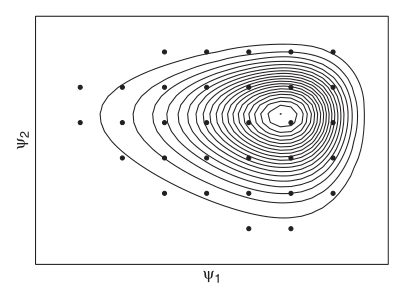
\includegraphics{images/CCDapplied.PNG}
\caption{CCD to spdetoy dataset, source \citet{Blangiardo-Cameletti}}
\end{figure}

The approximation \(\tilde{\pi}\left(\theta_{i} \mid y\right)\) can take different forms and be computed in different ways. \citet{Rue2009} also discuss how this approximation should be in order to reduce the numerical error \citep{Krainski-Rubio}.

Following \citet{Bayesian_INLA_Rubio}, approximations of the joint posterior for the hyper paramer \(\tilde\pi\left(\psi_{k} \mid \boldsymbol{y}\right)\) is used to compute the marginals for the latent effects and hyper parameters in this way:

\[
\left.\tilde{\pi}(\boldsymbol{\psi} \mid \mathbf{y}) \propto \frac{\pi(\boldsymbol{\theta}, \boldsymbol{\psi}, y)}{\tilde{\pi}_{G}(\boldsymbol{\theta} \mid \boldsymbol{\psi}, y)}\right|_{\boldsymbol{\theta}=\boldsymbol{\theta}^{*}(\boldsymbol{\psi})}
\]

In the previous equation \(\tilde{\pi}_{G}(\boldsymbol{\theta} \mid \boldsymbol{\psi}, y)\) is a gaussian approximation to the full condition of the latent effect \({\theta}^{*}(\boldsymbol{\psi})\) is the mode for a given value of the hyper param vector \(\boldsymbol{\psi}\)

At this point there exists three types of approximations for \(\pi\left(\boldsymbol{\theta} \mid \boldsymbol{\psi}, y\right)\)

\begin{itemize}
\tightlist
\item
  first with a gaussian approximation, estimating mean \(\mu_{i}(\boldsymbol{\psi})\) and variance \(\sigma_{i}^{2}(\boldsymbol{\psi})\).
\item
  second using the \emph{Laplace Approximation.}
\item
  third using \emph{simplified Laplace Approximation}
\end{itemize}

(rivedere meglio)

\hypertarget{rinla}{%
\section{R-INLA package in a bayesian hierarchical regression perspective}\label{rinla}}

\hypertarget{overview}{%
\subsection{Overview}\label{overview}}

INLA computations and methodology is developed by the R-INLA project whose package is available on their \href{http://www.r-inla.org}{website}. Download is not on CRAN (the Comprehensive R Archive Network) so a special source repo link, which is maintained by authors and collaborators, has to be optioned. The website offers also a forum where a daily discussion group is opened and an active community is keen to answer. Moreover It also contains a number of reference books, among which some of them are fully open sourced as gitbook. Furthermore as Havaard Rue has pointed out in a web-lecture on the topic, the project is gaining importance due to its new applications and recent use cases, but by no means it is replacing the older MCMC methods, rather INLA can integrate pre existing procedures.
The core function of the package is \texttt{inla()}and it works as many other regression functions like \texttt{glm()}, \texttt{lm()} or \texttt{gam()}. Inla function takes as arguments the formula (where are response and linear predictor), the data (expects a data.frame obj) on which estimation is desired together with the distribution of the data. Many other methods inside the function can be added through lists, such as \texttt{control.family} and \texttt{control.fixed} which let the analyst specifying priors distribution both for \(\boldsymbol{\theta}\) parameters, \(\boldsymbol{\psi}\) hyper parameters and the outcome precision \(\tau\), default values are non-informative.
\texttt{control.fixed} as said regulates prior specification through a plain list when there only a single fixed effect, instead it does it with nested lists when fixed effects are greater than 2, a guided example might better display the behaviour:
\texttt{control.fixed\ =\ list(mean\ =\ list(a\ =\ 1,\ b\ =\ 2,\ default\ =\ 0))}
In the chuck above it is assigned prior mean equal to 1 for fixed effect ``a'' and equal 2 for ``b''; the rest of the prior means are set equal to 0.
Inla objects are inla.dataframe summary-type lists containing the results from model fitting. Results contained in the object are specified in the table below, even though some of them requires special method: (se riesco più elegante in kable)
Following Krainski \& Rubio \citeyearpar{Krainski-Rubio} observations \(y(s_{1}), \ldots, y(s_{n})\) are taken from a toy generated dataset and a hierarchical linear regression is fitted.

\begin{figure}
\centering
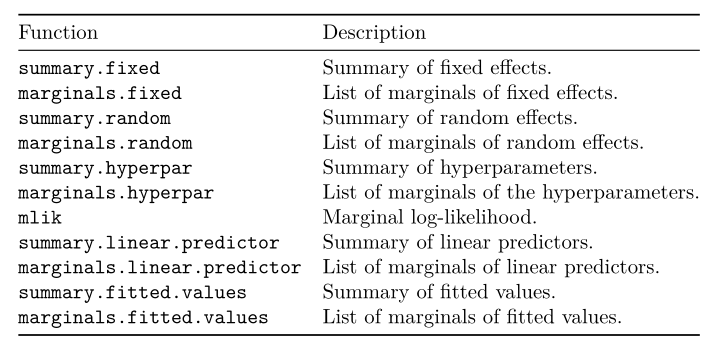
\includegraphics{images/summarytable.PNG}
\caption{summary table list object, source: \citet{Krainski-Rubio}}
\end{figure}

\hypertarget{example}{%
\subsection{Linear Predictor}\label{example}}

SPDEtoy dataset, that has a spatial component, is generated from a \(y_{i}\) Gaussian variable; its moments are \(\mu_{i}\) and precision \(\tau\).

\begin{figure}
\centering
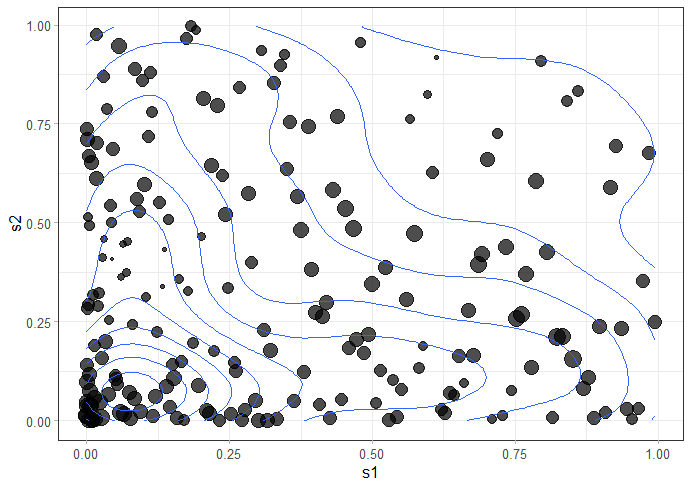
\includegraphics{images/cotour_toy.png}
\caption{SPDEtoy plot, author's source}
\end{figure}

The formula that describe the linear predictor has to be called directly inside the \texttt{inla()} function or it can be stored in the environment into a variable. The mean moment in the gaussian distribution \(\mu_{i}\) is expressed as the \emph{linear predictor} \(\eta_{i}\) (i.e.~\(E\left(y_{i} \mid \beta_{0}, \ldots, \beta_{M}, x_{i 1}, \ldots, x_{i M}\right) = \eta_{i}\) ). The function that maps the linear predictor into the parameter space is identity as in the initial part of section \ref{LGM} i.e.~\(\eta_{i}=\beta_{0}+\sum_{m=1}^{M} \beta_{m} x_{m i}+\sum_{l=1}^{L} f_{l}\left(z_{l i}\right)\).
After including \(s_{1}\) and \(s_{2}\) spatial covariates the linear predictor takes the following form: \(\beta_{0}+\beta_{1} s_{1 i}+\beta_{2} s_{2 i}\), where once again \(\beta_{0}\) is the fixed effect i.e.~intercept and the \(\beta_{j}\) are the linear effect on covariates. INLA allows also to include non-linear effects with the \texttt{f()} method inside the formula. \texttt{f} are foundamental since they are used to incorporate the spatial component in the model through the Matérn covariance function, this will be shown in section (boh).
Once the formula is decided then priors has to be picked up; for the intercept a customary choice is uniform. Prior for Gaussian latent parameters are vague and they have 0 mean and 0.001 precision, then the prior for \(\tau\) is a Gamma with parameters 1 and 0.00005. Prior initial choice can be later adapted.

The summary of the model parameters is:

\[
\begin{aligned}
y_{i} & \sim N\left(\mu_{i}, \tau^{-1}\right), i=1, \ldots, 200 \\
\mu_{i} &=\beta_{0}+\beta_{1} s_{1 i}+\beta_{2} s_{2 i} \\
\beta_{0} & \sim \text { Uniform } \\
\beta_{j} & \sim N\left(0,0.001^{-1}\right), j=1,2 \\
\tau & \sim G a(1,0.00005)
\end{aligned}
\]

\begin{Shaded}
\begin{Highlighting}[]
\KeywordTok{data}\NormalTok{(}\StringTok{"SPDEtoy"}\NormalTok{)}
\NormalTok{formula =}\StringTok{ }\NormalTok{y }\OperatorTok{~}\StringTok{ }\NormalTok{s1 }\OperatorTok{+}\StringTok{ }\NormalTok{s2}
\NormalTok{m0 =}\StringTok{ }\KeywordTok{inla}\NormalTok{(formula, }\DataTypeTok{data =}\NormalTok{ SPDEtoy)}
\end{Highlighting}
\end{Shaded}

\begin{tabular}{lrrrrrrr}
\toprule
  & mean & sd & 0.025quant & 0.5quant & 0.975quant & mode & kld\\
\midrule
(Intercept) & 10.1321487 & 0.2422118 & 9.6561033 & 10.1321422 & 10.6077866 & 10.1321497 & 7e-07\\
s1 & 0.7624296 & 0.4293757 & -0.0814701 & 0.7624179 & 1.6056053 & 0.7624315 & 7e-07\\
s2 & -1.5836768 & 0.4293757 & -2.4275704 & -1.5836906 & -0.7404955 & -1.5836811 & 7e-07\\
\bottomrule
\end{tabular}

The output offers among the others a summary of the posterior marginal values for intercept, coefficient and covariates, as well as precision. Below the plots for the parameters and hyperparameters. From the summary it can be seen that the mean for s2 is negative, so the more the value of the y-coordinates increases the more the output decreases, that is truer looking at the SPDEtoy cotour plot. Plots can be generated by calling the \texttt{plot} function on the inla object, however the one generated below are \texttt{ggplot2} outputs coming from the \$marginals.fixed list object.

\begin{figure}
\centering
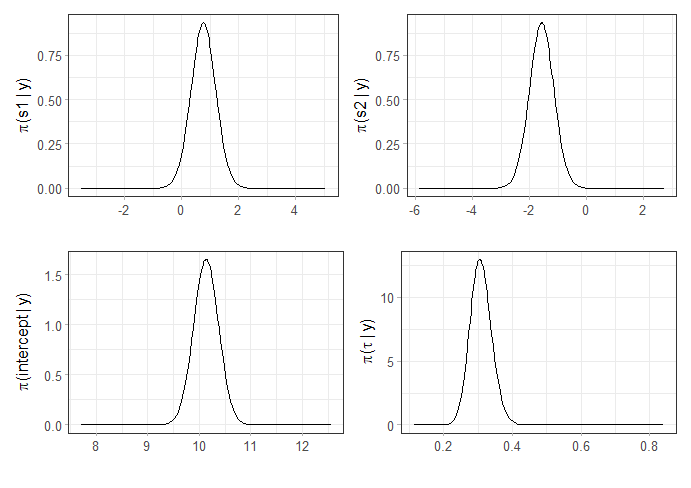
\includegraphics{images/marginal_distr.png}
\caption{linear predictor marginals, author's creation}
\end{figure}

R-Inla also has r-base fashion function to compute statistics on marginal posterior distributions for the density, distribution as well as the quantile function respectively \texttt{inla.dmarginal}, \texttt{inla.pmarginal} and \texttt{inla.qmarginal}. One major option which is conveniently packed into a dedicated function computes the higher posterior density credibility interval \texttt{inla.hpdmarginal} for a given covariate's coefficient, such that \(\int_{q_{1}}^{q_{2}} \tilde{\pi}\left(\beta_{2} \mid \boldsymbol{y}\right) \mathrm{d} \beta_{2}=0.90\) zwith .1 Confidence Level, in table @ref(tab:higer\_posterior\_density\_interval).

\begin{tabular}{lrr}
\toprule
  & low & high\\
\midrule
level:0.9 & -2.291268 & -0.879445\\
\bottomrule
\end{tabular}

Recall that the interpretation is different from the frequentist: in Bayesian statistics \(\beta_{j}\) comes from probability distribution, while frequenstists considers \(\beta_{j}\) as fixed unknown quantity whose estimator (random variable conditioned to data) is used to infer the value \citeyearpar{Blangiardo-Cameletti}.

\hypertarget{prdm}{%
\chapter{Point Referenced Data Modeling}\label{prdm}}

Geostatistical data are a collection of samples of geo type data indexed by coordinates (e.g.~latlong, eastings and northings) that originate from a spatially continuous phenomenon \citep{Moraga2019}. Data as such can monitor a vast range of phenomena, as an example disease cancer detection \citep{Bell2006} at several sites, COVID19 spread in China \citep{Li_Li_Ding_Hu_Chen_Wang_Peng_Shen_2020}, PM pollution concentration in a North-Italian region Piemonte \citep{Cameletti2012}. Moreover house prices variation, as observed in \citet{Bayesian_INLA_Rubio}, where selling prices smoothly vary between closer neighborhoods. All the Examples taken before might document a spatial nature of data according to which closer observations can display similar values, this phenomenon is named spatial autocorrelation. Spatial autocorrelation conceptually originates from geographer Waldo Tobler whose famous quote, known as first law of geography, inspires geostatisticians:

\begin{quote}
``Everything is related to everything else,
but near things are more related than distant things''

\hfill --- Waldo R. Tobler
\end{quote}

Spatial models are explicitly designed to take into account this behavior and can separate spatial patterns from simply random spatial variance.
Spatial data can be partitioned into three spatial data type whose modeling tools are specific with respect to their category.

\begin{itemize}
\tightlist
\item
  Areal Data
\item
  \textbf{Point Referenced Data}
\item
  Point Pattern Data
\end{itemize}

\begin{figure}
\centering
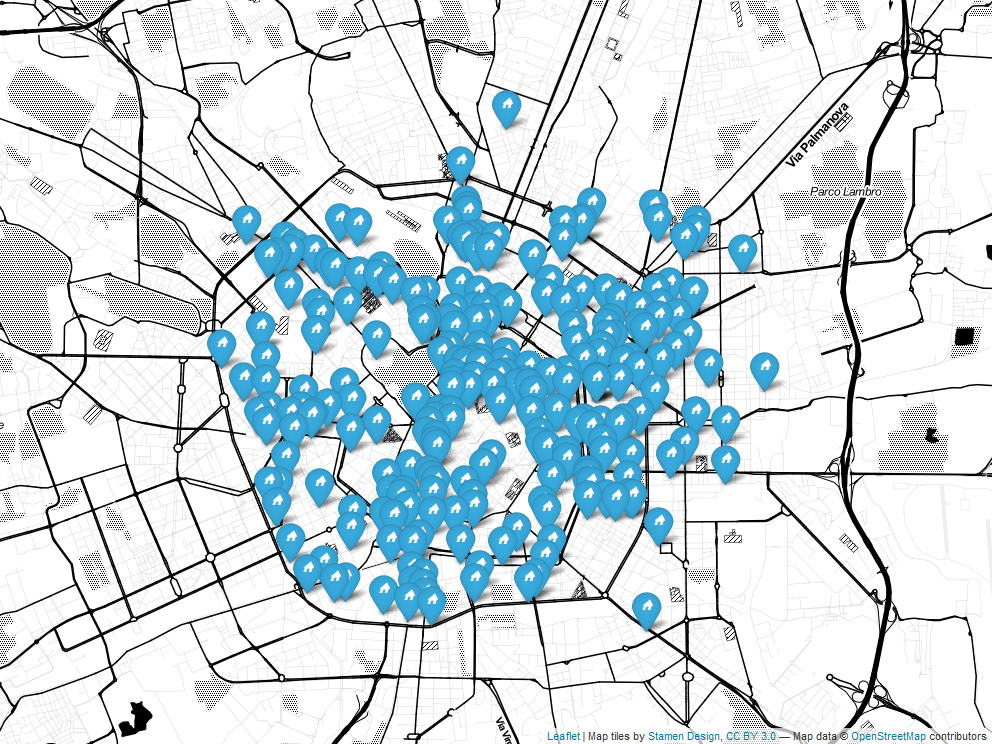
\includegraphics{images/map.png}
\caption{point referenced data example, Milan Rental Real Estate, Author's Source}
\end{figure}

REST API seen in chapter \ref{Infrastructure} extracts point referenced data, so modeling methodologies described in this analysis will exclusively take into account point referenced oriented techniques.
In order to extend the notion from discrete measurements (i.e.~point referenced) to a continuous spatial surface a stochastic process, namely Gaussian Process, has to be introduced and constrained according to convenient properties. GP are then evaluated with a specific covariance function, i.e.~Matèrn. The reason why Matérn is selected as candidate for covariance function will be much more clear in the next chapter \ref{spde}.
Hedonic Price Models are at first introduced and then a brief literature review is offered. Hedonic Prices brings to this work the theoretical basis but they do not suggest estimation methods, which are essentially the major issue in geostatistics. For this reason Hedonic Models are exploited into a spatial bayesian regression framework with the aim to apply INLA (seen in chpater \ref{inla}) methodology.
At first standard Bayesian regression is presented as introduction, then the spatial component in the form of a GP is added to the model. Many parameters are considered so far, as a consequence a hierarchy structure is imposed. To this extent an entire section is dedicated to hierarchy which simplifies model building and methodology understanding as well as allowing to bring in many different parameters that come from different levels through the exchangeability property.
As a matter of fact parameters originate from the Gaussian latent field, but also from Matérn covariance function tuning hyper parameters.
Then INLA is applied and a GMRF representation of GP is\ldots{}
Spatial kriging is essential to predict the process at new locations so that the spatial surface can be plotted and analyzed.
In the end models have to be checked and verified with resampling schemes which are once again specific to the data type and the scope of the analysis.

\emph{(forse mettere alla fine come further developments)}
As a side note Spatial data can also be measured according to a further dimension which is the Time. Latest literature suggests that spatio temporal models are the most accurate, as a consequence it might be interesting to research time correlation between subsequent spatial data time points, a valuable reference is offered in \citet{PACI2017149}. This will not take an enormous effort due ti the fact that on a daily basis REST API generates data which are stored as .json file on a DB. Future research on this data might consider the idea to include the time component in the model.

\hypertarget{GP}{%
\section{Gaussian Process (GP)}\label{GP}}

For simplicity lets consider \(y\) point of interest observations \(y\left(\boldsymbol{s}_{1}\right),y\left(\boldsymbol{s}_{2}\right), \ldots, y\left(\boldsymbol{s}_{n}\right)\)
from a random spatial process \(Y\), such that: \(Y\left(\boldsymbol{s}_{1}\right),Y\left(\boldsymbol{s}_{2}\right), \ldots, Y\left(\boldsymbol{s}_{n}\right)\) observed at location \(\boldsymbol{s}_{1}, \ldots, \boldsymbol{s}_{n}\). In the context of geostatistical data each observation has to be considered as a partial realization of an unobserved random spatial process.
\(\left\{Y(s): s \in D \subset \mathbb{R}^{2}\right\}\), where surface \(D\) is a subset of r-dimensional Euclidean space \(\mathbb{R}^{r}\).
Moreover When \(r = 1\) it is the most simple stochastic process widely explored in literature i.e.~time series process. However geostatistical data always have \(r = 2\) (i.e.~lat and long, eastings and northings) or eventually \(r = 3\), when elevation data is available. The stochastic process \(Y\) is observed in a fixed set of ``monitoring stations'' and inference can be done regarding moments of the realized process. This information are essential to build a spatially continuous surface over the y-studied variable in order to predict the phenomenon at locations not yet observed.

\begin{figure}
\centering
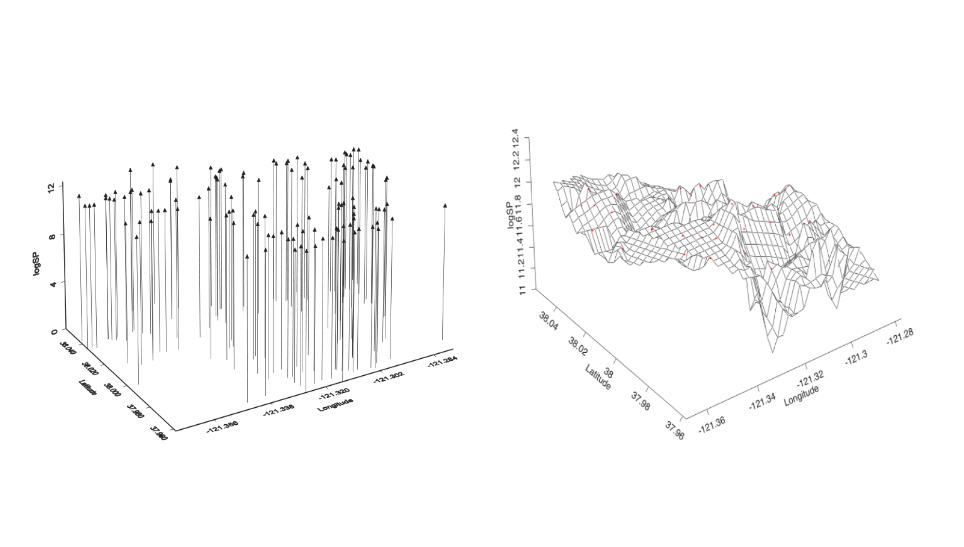
\includegraphics{images/prdprocess.png}
\caption{3D scatterplot and surface, Stockton data.}
\end{figure}

\begin{definition}[GP definition]
\protect\hypertarget{def:GP}{}{\label{def:GP} \iffalse (GP definition) \fi{} }A collection of \(n\) random variables, such as \(Y(s_{1}), Y(s_{2}) , \ldots, Y(s_{n})\) that are \emph{valid} spatial processes are said to be a \textbf{GP} if for any set of spatial index \(n\) and for each set of corresponding locations \(\left\{y\left(s_{1}\right), \ldots, y\left(s_{n}\right)\right\}\) follows a multivariate \emph{Gaussian} distribution with mean \(\boldsymbol{\mu}=\left\{\mu\left(s_{1}\right), \ldots, \mu\left(s_{n}\right)\right\}\) and covariance matrix \(\mathbf{Q}^{-1}_{i,j}, \forall i \neq j\)
\end{definition}

Even tough sometimes it is more convenient to express the covariance matrix as its inverse i.e.~precision matrix \(\boldsymbol{Q}_{i,j}\) \citep{Blangiardo-Cameletti}. The covariance matrix relates each observation to each of the others through a covariance function defined as \(\mathcal{C}(\cdot)\).

GP in the spatial context must check two important properties in order to exploit INLA, even though both of these assumptions can be relaxed:

\begin{itemize}
\tightlist
\item
  \textbf{Stationary}.
\item
  \textbf{Isotropy}.
\end{itemize}

\textbf{Stationarity} in a stochastic process can be \emph{strong}, \emph{weak} or \emph{intrinsic}. The strong property forces the distribution of the process \(\left\{y\left(s_{1}\right), \ldots, y\left(s_{n}\right)\right\}\) for any given spatial index \(n\) and its correspondent location sets \(s_{1,\ldots,n}\) to be the same as the one in \(\left\{y\left(s_{1}+\boldsymbol{h}\right), \ldots, y\left(s_{n}+\boldsymbol{h}\right)\right\}\), where \(h\) is a number belonging to \(R^{2}\).
On the other hand the weak property ensures that if the GP mean moment is constant over the study domain \(\mu(\mathbf{s}) \equiv \mu\) (e.g.~\(E[Y(s)]=\mu, \forall s \in D\)) then the covariance functions does depend only on the distance (euclidean \(\left\|s_{i}-s_{j}\right\|\) distance) between each couple points.
Weak stationarity consequences are the most interesting: It does not matter whether observations are placed either in a specific region, nor the direction towards they are oriented, the covariance functions \(\mathcal{C}(h)\) can summarize the process through the separation vector \(\mathbf{h}\) i.e.~\(\mathcal{C}(\mathbf{s}, \mathbf{s}+\mathbf{h})=\mathcal{C}(\mathbf{h}), \forall \mathbf{h} \in \mathbb{R}^{r}\) \citep{Banerjee-Gelfand}. In other words weak stationarity in GP implies being invariant under \emph{translation} \citeyearpar{Krainski-Rubio}. The relationship between strong and weak is not bijective since being strong implies also being weak, but the opposite is not always true for non-Gaussian process.
Furthermore through the intrinsic stationary property it is meant that \(E[Y(\mathbf{s}+\mathbf{h})-Y(\mathbf{s})]=0\), the second moment of the latter expression can be written as \(E[Y(\mathbf{s}+\mathbf{h})-Y(\mathbf{s})]^{2}\) leading to \(\operatorname{Var}(Y(\mathbf{s}+\mathbf{h})-Y(\mathbf{s}))\). Last expression is called \emph{variogram} and can be expressed with \(2 \gamma(\mathbf{h})\), even tough its half,i.e.~\(\gamma(\mathbf{h})\), is more interpretable, namely \emph{semivariogram} \citep{Cressie_2015}.

Semivariograms are characterized by mainly 3 tuning parameters:

\begin{itemize}
\tightlist
\item
  \emph{range} \(\sigma^{2}\): At some offset distance, the variogram values will stop changing and reach a sort of ``plateau''. The distance at which the effect occurs is called the range \(\frac{\Delta\gamma(\mathrm{h})}{h} \approx 0\).
\item
  \emph{sill} \(\tau^{2}\): The ``plateau'' value at which the variogram stops changing \(\frac{\Delta\gamma(\mathrm{h})}{h} = 0\).
\item
  \emph{nugget} \(\tau^{2}+\sigma^{2}\): The discontinuity at the origin. Although this theoretically should be zero, sampling error and short scale variability can cause it to be non-zero \(\gamma(\mathrm{0})\).
\end{itemize}

\begin{figure}
\centering
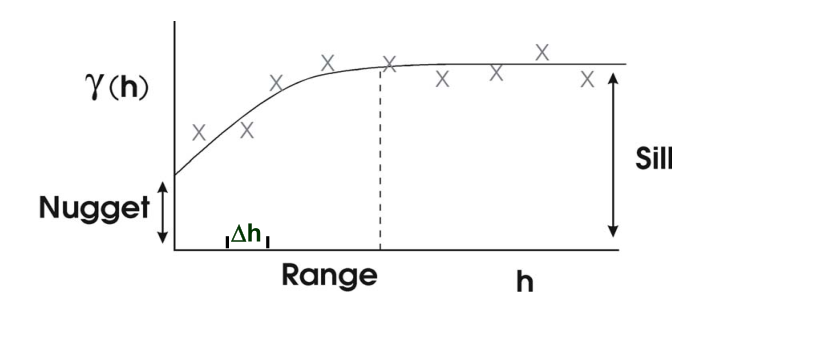
\includegraphics{images/variogram.png}
\caption{variogram example}
\end{figure}

presi i dati con le relative distanze euclidee a coppie di punti si binnano le distanze grazie ad un offset ottenendo i valori per il semivariogram. ottenuti i valori si fitta il semivargiogram a quei valori, un modo è la likelihood. A questo punto si calcolano le tre grandezze nugget sill e range per poi poter far uscire le funzioni di covarianza.

The process is said to be \textbf{Isotropic} if the covariance function depends only on the between-points distance \(\left\|\mathbf{h}\right\|\) so it is invariant under \emph{rotation} \citeyearpar{Krainski-Rubio}. A further way of seeing the property is that Isotropy implies concentric decaying contours that resemble the vanishing of spatial dependence, and so covariance values too.
then if the last assumption does not hold and direction towards point are distant from each other matters within the spatial domain \(D\), then is said to be \textbf{Anisotropic}.
Formalizing the results:

\[\mathcal{C}(\mathbf{h})=\mathcal{C}(\|\mathbf{h}\|)\]

\begin{figure}
\centering
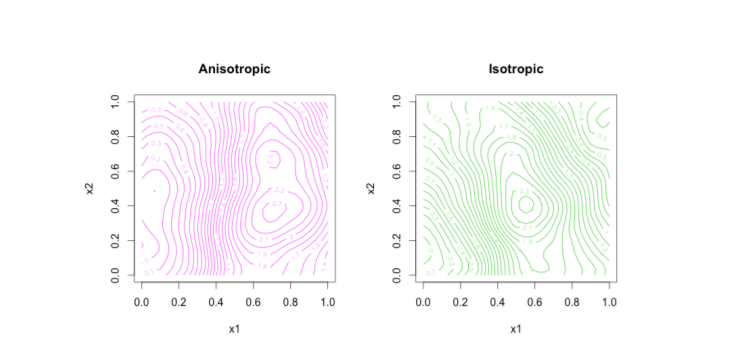
\includegraphics{images/isotropyVSanisotropy.png}
\caption{isotropy VS anisotropy, source \citet{blanchetscalliet}}
\end{figure}

\hypertarget{spatial-covariance-function}{%
\section{Spatial Covariance Function}\label{spatial-covariance-function}}

The covariance function \(\mathcal{C}(\cdot)\) ensures that all the values that are close together in input space will produce output values that are close together. \(\mathcal{C}(\cdot)\) needs to inherits the \emph{validity} characteristics from the random spatial process, furthermore it has to be \emph{positive definite}.
In addition covariance function must share characteristic properties of functions, such as:

(cerca di capire queste\ldots)

\begin{itemize}
\tightlist
\item
  Multiply valid covariance functions (summing independent random variables)
\item
  Mixing covariance functions (mixing distributions)
\item
  Convolving covariance functions, this will be very important \ldots{}
\end{itemize}

Covariance functions under stationary and isotropic GPs displays two important properties: they are constant in mean within \(D\) i.e.~\(\mathcal{C}(\mathbf{s}, \mathbf{s}+\mathbf{h})=\mathcal{C}(\mathbf{h}), \forall \mathbf{h} \in \mathbb{R}^{r}\) and they depends on distance vector \(\mathbf{h}\), not direction i.e.~\(\mathcal{C}(\mathbf{h})=\mathcal{C}(\|\mathbf{h}\|)\)
There are many covariance functions and ways to relate distant points on a spatial domain \(D\). Typically the choice of the Covariance can depend either on data or the scope of the analysis. Covariance functions are wrapped into special hyper parameters which are mainly three:

\begin{enumerate}
\def\labelenumi{\arabic{enumi}.}
\tightlist
\item
  \emph{Range}: At some offset distance, the variogram values will stop changing and reach a ``plateau''. The distance at which this occurs is called the range.
\item
  \emph{Sill}: The ``plateau'' value at which the variogram stops changing.
\item
  \emph{Nugget}: The discontinuity at the origin. Although this theoretically should be zero, sampling error and short scale variability can cause it to be non-zero
\end{enumerate}

(espressione della covariance function insieme a alle \(\sigma^2\) come: \(C(\mathbf{s}+\mathbf{h}, \mathbf{s} \mid \theta)=\sigma^{2} \mathbf{R}(\|h\| ; \phi)\))
spiega anche queste due sotto

\[
\mathbf{w}=\left(w\left(\mathbf{s}_{1}\right), \ldots, w\left(\mathbf{s}_{n}\right)\right)^{\prime} \sim \mathrm{N}\left(\mathbf{0}, \sigma^{2} \mathbf{R}(\phi)\right) \text { where } \left.\mathbf{R}(\phi)_{i j}=\rho\left(\left\|\mathbf{s}_{i}-\mathbf{s}_{j}\right\| ; \phi\right)\right)
\]

\(\Sigma_{\theta}=\sigma^{2} \mathbf{R}(\phi)+\tau^{2} I_{n}\)

A summary of the most used covariance functions are presented below.

\[
\begin{aligned}
&\text { Exponential } \quad \mathcal{C}(\mathbf{h})=\left\{\begin{array}{cl}
\tau^{2}+\sigma^{2} & \text { if }  h=0 \\
\sigma^{2} \exp (-\phi h) & \text { if } h>0 
\end{array}\right.\\
&\text { Gaussian } \quad \mathcal{C}(\mathbf{h})=\left\{\begin{array}{cl}
\tau^{2}+\sigma^{2} & \text { if } h=0 \\
\sigma^{2} \exp \left(-\phi^{2} h^{2}\right) & \text { if } h>0 
\end{array}\right. \\
&\text { Matérn } \quad \mathcal{C}(\mathbf{h})=\left\{\begin{array}{cl}
\tau^{2}+\sigma^{2} & \text { if } h=0 \\
\frac{\sigma^{2}}{2^{\nu-1} \Gamma(\nu)}(\phi h)^{\nu} K_{\nu}(\phi h) & \text { if } h>0
\end{array}\right.
\end{aligned}
\]

\hypertarget{Matern}{%
\subsection{Matérn Covariance Function}\label{Matern}}

Matérn is special since when it is used together with a stationary and isotropic GP, the SPDE approach can provide a GMRF representation of the same process, chapter \ref{spde} discloses this fundamental property.
Matérn can also be accounted as the most used in geostatistics \citep{Krainski2018} and \citep{Bayesian_INLA_Rubio} and is tuned mainly by two parameters, a scaling one \(\kappa>0\), usually set equal to the range by the relation \(\sigma^{2}=\frac{\sqrt{8 \lambda}}{\kappa}\)) and a smoothing one \(\nu>0\). A \emph{stationary} and \emph{isotropic} Matérn covariance function has this form:

\[
\mathcal{C}(\mathbf{h})=\left\{\begin{array}{ll}
\tau^{2}+\sigma^{2} & \text { if } h=0 \\
\frac{\sigma^{2}}{2^{\nu-1} \Gamma(\nu)}(\phi t)^{\nu} K_{\nu}(\phi t) & \text { if } h>0
\end{array}\right.
\]

\(\Gamma(\nu)\) is a Gamma function depending on \(\nu\) values, \(K_{\nu}(\cdot)\) is a modified Bessel function of second kind. The smoothness parameter \(\nu\) in the figure below takes 4 different values showing the potentiality of Matérn to relates distances to covariance values. When \(\nu = 1\) \ldots{} When \(\nu = 1/2\) it becomes the exponential covariance function, When \(\nu = 3/2\) it uncovers a convenient closed form, when \(\nu \approx \infty\), in this case for representation purposes \(\nu = 80\) it becomes Gaussian covariance function.

\begin{figure}
\centering
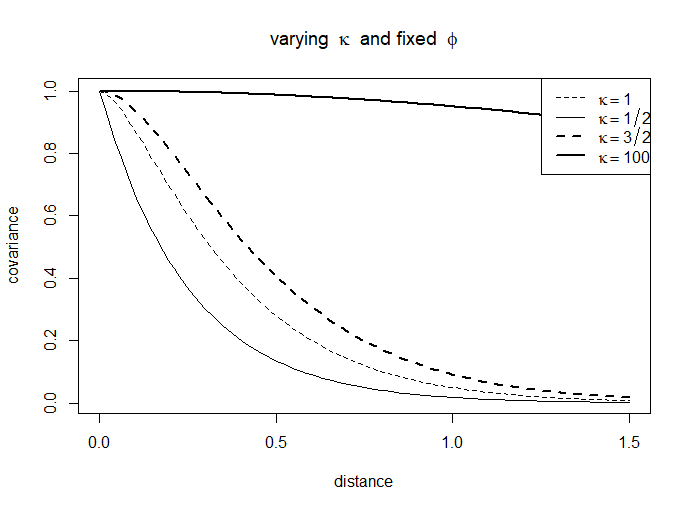
\includegraphics{images/matern.png}
\caption{matern correlation function for 4 diff values of nu with phi fixed, author's source}
\end{figure}

ancora di più su matern, forse di più in spde

\hypertarget{hedonic-models-literature-review-and-spatial-hedonic-price-models}{%
\section{Hedonic models Literature Review and Spatial Hedonic Price Models}\label{hedonic-models-literature-review-and-spatial-hedonic-price-models}}

The theoretical foundation of the Hedonic Price Models (from now on HPM) resides in the consumer utility theory of \citet{Lancaster} together with \citet{Rosen} market equilibrium. According to Lancaster the utility of a commodity does not exist by itself, instead it exists as the sum of the utilities associated to its separable characteristics. Integrating Lancater, Rosen introduces HPM and suggests that each separate commodity characteristics are priced by the markets on the basis of supply and demand equilibrium. Applying HPM to Real Estate in a market context, from the buy side house prices (but also rents) are set as the unit cost of each household attributes, conversely from the selling side the expenditures associated to build of each them.
Formalizing the results, Hedonic Price \(P\) in Real Estate is expressed as a general \(f\) functional form that takes as input the house characteristics vector \(\mathbf{C}\).

\[P=f\left(c_{1}, c_{2}, c_{3}, \ldots, c_{n}\right)\]

Vector \(\mathbf{C}\) since now might contain a unidentified and presumably vast number of ungrouped characteristics. In this setting \citet{Malpezzi} tried to organize house features by decomposing \(\mathbf{C}\) into mutually exclusive and exhaustive subgroups. An overview of the vector components involved is given by \citet{Ling} according to which \(P\) represents the house price, \(S\) is the structural characteristics of the house, \(N\) represents the neighborhood characteristics, \(L\) signifies the locational characteristics, \(C\) describes the contract conditions and \(T\) is time. \(\beta\) is the vector of the parameters to be estimated. Then

\[P=f\left(S, N, L, C, T, \beta\right)\]

Historically a first attempt to include spatial effect in urban economic literature is provided by \emph{Alonso (1964) miss ref}. Its contribution was to raise voice on house prices (also rent) mainly depending on land price and a number of purely spatial covariates like CBD, the distance from City Business District. Other covariates were transport cost per kilometer and community income, even though they were defined also as spatial parameters through distances. The model proposed by Alonso is called monocentric since the centroid from which distances are calculated is only one. Moreover a first touch to spatial data thory was done since the CBD was defined as areal unit with well-defined boundaries of regular or irregular shape. However applications of the model were not convincing since empirical studies offered a different picture. Results instead displayed a Poly-centric areal structure (universities and Malls) which might be better explaining prices. The model also assumed that covariates like CBD are only informative within city center boundaries and then displayed no significance out of the core of the city. Poly-centric theory was also more coherent with the architectural and socio-economical evolution of cities during that times, therefore mono centric theory was then criticized and abandoned. Critics regarded also neighborhood quality measure and boundary problems \emph{Dubin (1987) miss ref}. Dubin for these reasons developed a model including areal effects in the error term since handling these covariates was posing several hard challenges. Areal data choice for Dubin was forced since he was interested in land values, geostatics interest was not a focus also due to the difficulties in gathering accurate data. Coming to recent literature a change in focus has been made by switching from theory based model to estimation methods. As a consequence to the change in focus \citet{Ling} said that practitioners should spend more time in variable selection and model specification with respect to their specific need.
As Ling has observed the emerging trends are in the field of semi-parametric and non-parametric methods \citeyearpar{Ling}. Historically semi-parametric regression considers models indexed by spatial coordinates \emph{Pace RK (1995)}. At the same time \emph{Kammann and Wand (2003)} gave birth to geoadditive models where the spatial component is added as a covariate. {[}\ldots{]}

A further aspect of the problem is posed by scholars that do not consider rents to be representative for the actual value of real estate. Nevertheless in empirical analysis rent value are considered a proxy for real estate pricing \citep{Herath_Maier_2011}. A further argument to endorse this hypothesis is brought by \citet{sellingVSrental} considering housing a commodity, then the selling or the rental should be considered interchangeable economic actions with respect to same inner need to be satisfied. This is also truer to the thesis' extent since Manganelli, Morano, and Tajani have centered their analysis exactly on italian real estate data. Moreover \citet{Capozza_Seguin_1996} discussed on how much rent-price ratio predicts future changes both in rents and prices. Among all the other discussions raised they brought the decomposition of rent-price ratio into two parts: the predictable part and the unexplained residuals part. The predictable part was discovered to be negatively correlated with price changes, in other words cities in which prices are relatively high with respect to rents are associated with higher capital gains that might justify that misalignment. This is also true for the opposite, that is cities in which prices are lower with respect to the rents, and this effect can not be associated to any local condition, realize lower capital gains. A further argument is offered by Clark \citep{Clark_1995} which went after the Capozza and Seguin work. Rent-price ratio is negatively correlated with following future changes in rents. In other words prices are still higher when areas in which they are observed documents an increase in rent prices. All the literature review above is oriented to a long-run alignment of price and rent.

\hypertarget{univariateregr}{%
\section{Point Referenced Regression for univariate spatial data}\label{univariateregr}}

Since in HPM the relationships between the characteristics of the house, i.e.~vector \(\mathbf{C}\) and the price \(P\) is not in any case fixed by econometric literature it is possible to assume any \(f\) functional form. The open possibility to apply a wide range of relationship between covariates fit in the INLA setting, since Latent Gaussian Models are prepared to accept a any linear and non linear \(f\) functions \ref{LGM} through the \texttt{f()} method. Hedonic price models are, as a consequence, a subset of models that can be fitted into LGM and therefore by INLA method.

Moreover what the vast majority of econometric literature \emph{(Greene, 2018)} suggest to apply a is log-linear / square root model. This is due to the fact that log transformation / square root smooths the skewness of prices normalizing the curve, leading to more accurate estimates. Having an exponential family generating process lowers even further computational cost for reasons linked to the \(\tilde\pi(\boldsymbol{\psi})\) hyper param INLA approximation \citep{Blangiardo-Cameletti}. Notation is taken from the previous chapter \ref{inla}, for brevity purposes \(\boldsymbol{\beta}\) \(\mathbf{X}\) and \(\boldsymbol{y}\) indicates vectors incorporating all their respective realizations and the \(s\) spatial component is left out in favor of the observation pedix \(i\).\\
The simplest log-linear bayesian regression model assumes linear relationship between predictors and a Normal data generating process: (log has been taken out for simplicity, bu it will be then considered in the regression setting) (valuta l'idea che per interpretabilità di modellarla come Gamma exponential family anzichè tenerla normale)

\[
\log{(y_{i})} \sim \operatorname{Normal}(\mu_{i}, \sigma^{2})
\]

\[
y_{i}=\mu_{i}+\varepsilon_{i}
\]

then by the following relationship \(E\left(y_{i} \mid \beta_{0}, \ldots, \beta_{M}, x_{i 1}, \ldots, x_{i M}\right)=\beta_{0}+\sum_{m=1}^{M} \beta_{m} x_{i m}\) it is possible to specify a more general linear predictor (seen also in chapter \ref{inla}) through an identity link function i.e.~\(\eta_{i}=g\left(\mu_{i}\right)=\mu_{i}\) obtaining:

\[
\eta_{i}=\beta_{0}+\sum_{m=1}^{M} \beta_{m} x_{m i}+\sum_{l=1}^{L} f_{l}\left(z_{l i}\right)
\]

Where, once again, the mean structure linearly depends on some \(\mathbf{X}\) covariates, \(\boldsymbol{\beta}\) coefficients, \(f_{l}(\cdot), \forall l \in 1 \ldots L\) are a set of random effects defined in terms of a \(\boldsymbol{z}\) set of covariates \(\boldsymbol{z}=\left(z_{1}, \ldots, z_{L}\right)\) (e.g.~rw, ar1) and \(\varepsilon_{i}\) white noise error.
Priors have to be specified and a non informativeness for \(\tau^2 = 1/\sigma^2\) and \(\boldsymbol{\beta}\) is chosen, such that \(\pi(\tau^2) \propto 1\) and \(\pi(\boldsymbol\beta) \propto 1\). As a consequence the conditional posterior for the parameters of interest \(\boldsymbol{\beta}\) is:

\[
\boldsymbol{\beta} \mid \sigma^{2}, \boldsymbol{y}, \boldsymbol{X} \sim \operatorname{MVNormal}\left(\left(\boldsymbol{X}^{\prime} \boldsymbol{X}\right)^{-1} \boldsymbol{X}^{\prime} \boldsymbol{y}, \sigma^{2}\left(\boldsymbol{X}^{\prime} \boldsymbol{X}\right)^{-1}\right)
\]

where the mean structure corresponds to the OLS estimator: \(\left(\boldsymbol{X}^{\prime} \boldsymbol{X}\right)^{-1} \boldsymbol{X}^{\prime} \boldsymbol{y}\) for \(\beta\) and then to obtain the marginal posterior for \(\boldsymbol{\beta}\) it is needed to integrate with respect to \(\sigma^2\).

In order to engage the spatial coordinate components into the regression setting \(w_{i}\) has to be added to the equation. \(w_{i}\) is set as a stationary and isotropic GP with mean 0 and variance as covariance function expressed as Matérn.
Recall that GP
The new regression setting integrates the \emph{spatial error} part in the name of \(w_{i}\) and a \emph{non-spatial error} part \(\varepsilon_{i}\) distributed normally with mean 0 and variance \(\tau^2\) ,i.e.~\(\mathrm{N}\left(0, \tau^{2}\right)\), which offers its contribution error to the nuggets via the covariance function.
Consequently there is one more parameter to estimate. It is worth mentioning that the distribution of \(w_{i}\) at a finite number of points is considered a realization of a multivariate Gaussian distribution. In this case, the likelihood estimation is possible and it is the multivariate Gaussian distribution with covariance \(\Sigma\).

\[
\log(y_{i})= \beta_{0} + (\mathbf{X})^{\prime}\boldsymbol{\beta}+w_{i}+\varepsilon_{i}
\]

The covariance of the marginal distribution of \(y_{i}\) at a finite number of locations is \(\Sigma_{y} = \Sigma + \tau^2\mathbf{I}\), where \(\mathbf{I}\) denotes the indicator function (i.e., \(\mathbf{I}(i = i^{\prime})= 1\) if \(i = i^{\prime}\), and 0 otherwise). This is a short extension of the basic GF model, and gives one additional parameter to estimate

\hypertarget{hiermod}{%
\section{Hierarchical Bayesian models}\label{hiermod}}

Spatial Models are characterized by many parameters which in turn are tuned by other hyper-parameters. Traditionally Bayesian hierarchical models are not widely adopted since they have high computational burdens, indeed they can handle very complex interactions via random components, especially when dealing with spatio temporal data \citet{Ling}. Blangiardo e Cameletti \citeyearpar{Blangiardo-Cameletti} tried to approach the problem from a different angle offering an intuitive solution on how hierarchy relates different levels parameters. This is done by reversing the problem and starting from data back to parameters, instead the other way round. So taking a few steps back the problem can be reformulated by starting from grouping observation into categories and then trying to impose a hierarchical structure on data based on the categories. As a result observations might fall into different categories, underlining their natural characteristics, such as: some of them might belong to category \emph{levels} like males or females, married or not-married. Moreover diving into the specific problem house prices can be faceted by which floor they belong or whether they are assigned to different energy classes and many others more. As an example Blangiardo and Cameletti example consider grouping data according to just a single 9 \emph{levels} category. Data for the reasons stated before can be organized such that each single observation (squares in figure below) belongs to its respective mutually exclusive and collectively exhaustive category (circles in figure).

\begin{figure}
\centering
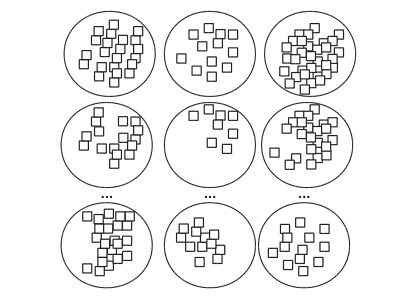
\includegraphics{images/simple.PNG}
\caption{9 levels cat vs observaitions, source \citet{Blangiardo-Cameletti}}
\end{figure}

Furthermore data can be partitioned into two meta-categories, \emph{fist level} and \emph{second level}, highlighting the parameter and hyper paramter chain roles. \emph{First level} are identified by sampling observations which are drawn by the same probability distribution (squares) . \emph{Second level} (circles) are categories and might be associated to a set of parameters \(\theta=\left\{\theta_{1}, \ldots, \theta_{J}\right\}\).
Since the structure is hierarchical, a DAG (Directed Acyclical Graph) \citeyearpar{Blangiardo-Cameletti} representation might sort out ideas. If categories are represented by different \(\theta_{j}\) nodes and edges (arrows in the figure) are the logical belonging condition to the category then a single parameter \(\theta\) model has the right figure form:

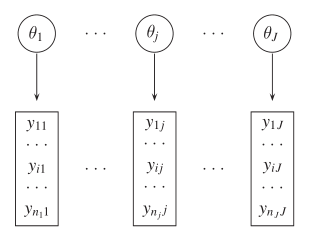
\includegraphics{images/thetas.PNG} 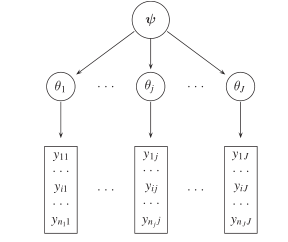
\includegraphics{images/chis.PNG}

To fully take into account the hierarchical structure of the data the model should also consider further lelvels. Since \(\left\{\theta_{1}, \ldots, \theta_{J}\right\}\) are assumed to come from the same distribution \(\pi(\theta_{j})\), then they are also assumed to be sharing information \citep{Blangiardo-Cameletti}, (left figure). When a further parameter \(\boldsymbol{\psi}=\left\{\psi_{1}, \ldots, \psi_{K}\right\}\) is introduced, for which a prior distribution is specified, then the conditional distribution of \(\boldsymbol{\theta}\) given \(\boldsymbol{\psi}\) is:

\[
\pi\left(\theta_{1}, \ldots, \theta_{J} \mid \boldsymbol{\psi}\right)=\int \prod_{j=1}^{J} \pi\left(\theta_{j} \mid \psi\right) \pi(\psi) \mathrm{d} \psi
\]
This is possible thanks to the conditional independence property already encountered in chapter \ref{inla}, which means that each single \(\theta\) is conditional independent given \(\psi\)
This structure can extended to allow more than two levels of hierarchy since the marginal prior distributions of \(\theta\) can be decomposed into the product of their conditional priors distributions given some hyper parameter \(\psi\) as well as their prior distribution \(\pi(\psi)\).

\[
\pi(\boldsymbol{\theta})=\int \pi\left(\boldsymbol{\theta} \mid \boldsymbol{\psi}_{1}\right) \pi\left(\boldsymbol{\psi}_{1} \mid \boldsymbol{\psi}_{2}\right) \ldots \pi\left(\boldsymbol{\psi}_{L-1} \mid \boldsymbol{\psi}_{L}\right) \pi\left(\boldsymbol{\psi}_{L}\right) \mathrm{d} \boldsymbol{\psi}_{1} \ldots \mathrm{d} \boldsymbol{\psi}_{L}
\]

\(\boldsymbol{\psi}_{l}\) identifies the hyper pram for the \(l_{th}\) level of hierarchy. Each further parameter level \(\psi\) is conditioned to its previous in hierarchy level \(l-1\) so that the parameter hierarchy chain is respected and all the linear combinations of parameters are carefully evaluated. The \emph{Exchangeability} property enables to have higher \(H\) nested DAG (i.e.~add further \(L\) levels) and to extend the dimensions in which the problem is evaluated, considering also time together with space. From a theoretical point of view there are no constraints to how many \(L\) levels can be included in the model, but as a drawback the more the model is nested the more it suffers in terms of interpretability and computational power. Empirical studies have suggest that three levels are the desired amount since they offer a good bias vs variance trade-off.

\hypertarget{finalregr}{%
\section{INLA model through spatial hierarchical regression}\label{finalregr}}

INLA model seen in section \ref{LGM} can be rearranged according to the hierarchical structure considering also the regression settings for point referenced data stated in the previous section \ref{univariateregr}.

As an initial step it is required to specify a probability distribution for \(\boldsymbol{y} = \left(y\left(s_{1}\right), \ldots, y\left(s_{n}\right)\right)=\left(y_{1}, \ldots, y_{n}\right)\), this is a mandatory step looking at the \ref{example} methods needed to compute the \texttt{inla()} function. A Normal distribution for simplicity is chosen.

As \emph{first level} is picked up an \textbf{exponential family} sampling distribution (i.e.~Normally distributed, Gamma one other choice), which is \emph{exchangeable} with respect to the \(\boldsymbol{\theta}=\left\{\beta_{0}, \boldsymbol{\beta}, f\right\}\) \emph{latent field} and hyper parameters \(\boldsymbol{\psi_{1}}\), which includes also the ones coming from the latent Matérn GP process \(w_{i}\). The Spatial Guassian Process is centered in 0 and with Matérn covariance function as \(\tau^2\). \(w_{i}\) addresses the spatial autocorrelation between observation through a Matérn covariance function \(\mathcal{C}(\cdot | \boldsymbol\psi_{1})\) which in turn is tuned by hyper param included in \(\boldsymbol{\psi_1}\). Moreover the \(w_{i}\) surface has to be passed in the formula method definition \ref{example} via the \texttt{f()} function, so that INLA takes into cosideration the spatial component.

\[
\boldsymbol{y} \mid \boldsymbol{\theta}, \boldsymbol{\psi}_{1} \sim \mathrm{N}\left(\beta_{0}+ (\mathbf{X}_{i})^{\prime}\boldsymbol{\beta} + w_{i} ,  \tau^2 I_{n}\right)=\prod_{i=1}^{n} \mathrm{N}\left(y_{i} \mid \theta_{i}, \psi_{1}\right)
\]

Then at the \emph{second level} the latent field \(\boldsymbol{\theta}\) is characterized by a Normal distribution given the remaining hyper parameters \(\boldsymbol{\psi}_2\), recall the covariance matrix \(\boldsymbol{Q}^{-1}(\boldsymbol{\psi_{2}})\), depending on \(\boldsymbol{\psi_{2}}\) hyperparameters, is handled now by a Matérn covariace function depeding on its hyperparamter. This is done in order to map the GP spatial surface into a GMRF by SPDE solutions.

\[
\boldsymbol{\theta} \mid \boldsymbol{\psi}_{2} \sim \mathrm{N}\left(\boldsymbol{0}, \mathcal{C}( \cdot , \cdot  \mid \boldsymbol{\psi}_{2})\right)
\]

In the end a \emph{third level} hyper parameters \(\boldsymbol{\psi}=\left\{\boldsymbol{\psi_{1}}, \boldsymbol{\psi}_{2}\right\}\) having some specified prior distribution i.e.~\(\boldsymbol{\psi} \sim \pi(\boldsymbol{\psi})\),

\hypertarget{spatial-kriging}{%
\section{Spatial Kriging}\label{spatial-kriging}}

In Geostatistics the main interest resides in the spatial prediction of the spatial latent field pr the response variable at location not yet observed.
Assumed the model in the previous section, suppose that \(y^{\star}\) is not a observed occurrence of the response variable at location \(s_{0}\) (not in the data) of the GP \(w_{i}\) spatial surface estimated through observed refereced points in \(\boldsymbol{y}\). As a consequence of exchangeability (first step previous section \ref{finalregr}) then \(\boldsymbol{y}^{\otimes}=\left\{\boldsymbol{y}, y^{\star}\right\}\). Then considering INLA notation it is obtained:

\[
\begin{aligned}
&\pi\left(y^{\star} \mid \boldsymbol{y}\right)=\frac{\pi\left(\boldsymbol{y}, y^{\star}\right)}{\pi(\boldsymbol{y})} \text { from the conditional probability }\\
&=\frac{\int \pi\left(y^{\star} \mid \theta\right) \pi(\boldsymbol{y} \mid \theta) \pi(\theta) \mathrm{d} \theta}{\pi(\boldsymbol{y})} \text { by exchangeability }\\
&=\frac{\int \pi\left(y^{\star} \mid \theta\right) \pi(\theta \mid y) \pi(y) \mathrm{d} \theta}{\pi(y)} \text { applying Bayes' theorem }\\
&=\int \pi\left(y^{\star} \mid \boldsymbol{\theta}\right) \pi(\boldsymbol{\theta} \mid \boldsymbol{y}) \mathrm{d} \boldsymbol{\theta}
\end{aligned}
\]

A DAG representation might offr the intuition behind Prediction in spatial models:

\begin{figure}
\centering
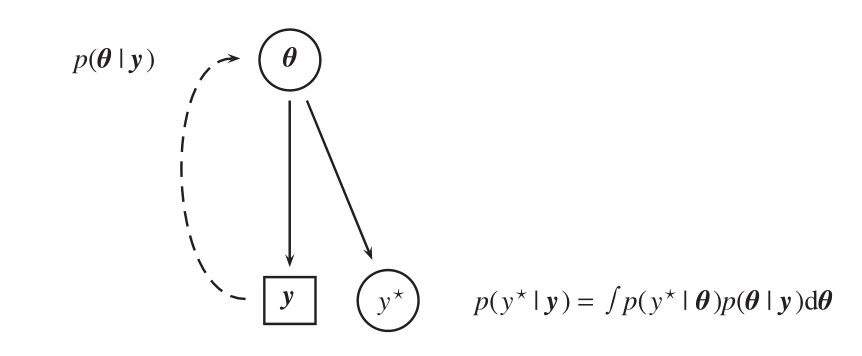
\includegraphics{images/spatial_prediction.jpg}
\caption{Spatial prediction representation through DAG, source \citet{Blangiardo-Cameletti}}
\end{figure}

where \(\pi\left(y^{\star} \mid \boldsymbol{y}\right)\) is said predictive distribution and it is meaningful only in the Bayesian framework since the posterior distribution is treated as a random variable, which is totally not true in frequentist statistics.

\hypertarget{model-checking}{%
\section{Model Checking}\label{model-checking}}

(Incrociarlo con altri tesi)

Once the model is set up and fitted a resampling scheme has to be chosen in order to evaluate the model performance. One of the most used method to assess beyasian model quality is LOOCV cross validation and defualt choice fo R-INLA package. From data is left out one single observation and so that the Validation set is \(\boldsymbol{y}_{v} = \boldsymbol{y}_{-i}\) and the Assessement set is a \(\boldsymbol{y}_{a} = \boldsymbol{y}_{i}\)
the rest of the observations. Two KPI are assumed to be representative:

\begin{itemize}
\tightlist
\item
  CPO conditional predictive ordinate (pettit, 1990): \(CPO_{i} = \pi(y^{\star} \mid \boldsymbol{y}_{v})\)
\item
  PIT probability integral tranform (dawid, 1984): \(PIT_{i} = \pi(y^{\star} < y_{i} \mid \boldsymbol{y}_{v})\)
\end{itemize}

These quantities are used by default by setting control options in the \texttt{inla(control.compute\ =\ list())} list object by setting them equal o TRUE. Inla also provides an inner method to authomatically handlee failing in computing those two quantities, leadind to values of 1 when predictions are not reliable and the ipposite for 0.Moreover the empirical distribution of the PIT can be used to asses predictive performance: if it is Uniform, so there are not values that strongly differ from the others then the model is correctly checked. Otherwise if the dostribtuon almost approxiamtes any of the other possibles then the Cross validation assessement prediction has led incorrectly predict the ``out of the bag'' validation sample.

Posteerior checking method exploits a full cross validation where \(\boldsymbol{y}_{a} = \boldsymbol{y}_{v}\) and it is called predictive checks. Th assessement set now is equal to the validation set,a s a consequence all the observation are evaluated twice. 4 quantities are driver to model estimate quality:

\begin{itemize}
\tightlist
\item
  the \emph{posterior predictive distribution}: \(\pi(y^{\star} \mid \boldsymbol{y}) = \int \pi(y^{\star} \mid \theta_{i})\pi({\theta_{i}} \mid \boldsymbol{y})\mathrm{d}\theta_{i}\) which is the likelihood of a replicate observation. When values are small that indicates that are those values are coming from tails, since the area under the curve (i.e.~probability) is less. If this happens for many observation then outliers are driving the model leading to poor estimates
\item
  the \emph{posterior predictive p-value} whose math expression is:\(\pi(y^{\star} \leq y_{i} \mid \boldsymbol{y})\) for which values near to 0 and 1 indicates poor perfomances.
\item
  \emph{Root Mean Square Predictive Error RMSE}: \(\sqrt{\frac{1}{n} \sum_{i=1}^{n}(y_{i}-{y}^{\star}_{i})^{2}}\)
\item
  \(R^2\)
\end{itemize}

R-INLA has already antiticipated in chapter 4 section\ref{example} have designed function to compute statistics on posterior distribution as \texttt{inla.pmarginal()} returning the cumulative density distribution.

\hypertarget{prior-specification}{%
\section{Prior Specification}\label{prior-specification}}

\hypertarget{spde}{%
\chapter{SPDE approach}\label{spde}}

Observations in the spatial problem setting are considered as realizations of a stationary, isotropic unobserved GP \(w(s)\) that we aim to estimate (\ref{GP}). Before approaching the problem with SPDE, GPs were treated as multivariate Gaussian densities and Cholesky factorizations were applied on the covariance matrices and then fitted with likelihood. Matrices in this settings were very dense and they were scaling with the order of \(O\left(n^{3}\right)\), leading to obvious big-n problem.
The breakthrough, came with \citet{Lindgren2011} that proves that a stationary, isotropic GP with Matérn covariance can be represented as a GMRF using SPDE solutions by finite element method \citep{Krainski-Rubio}. In other words given a GP whose covariance matrix is \(\boldsymbol{Q}\), SPDE can provide a method to approximate \(\boldsymbol{Q}\) without computational constraints. As a matter of fact SPDE are equations whose solutions are GPs with a chosen covariance function focused on satisfying the relationship SPDE specifies.
Benefits are many but the most important is that the representation of the GP through a GMRF provides a sparse representation of the spatial effect through a sparse precision matrix \(\boldsymbol{Q}^-1\) . Sparse matrices enable convenient inner computation properties of GMRF that can be exploited with INLA. Bayesian inference on GMRF can take advantage of lower computational cost because of these properties stated before leading to a more feasible big-O \(O\left(n^{3 / 2}\right)\). The following chapter will provide a intuition on SPDE oriented to practitioners. The chapeter once again will follow the track of Krainski \& Rubio \citeyearpar{Krainski-Rubio} and Blangiardo and Cameletti \citeyearpar{Blangiardo-Cameletti} works, together with the street-opener paper from \citet{Miller2019} as compendium. SPDE might be complex for those who are not used to applied mathematics and physics making it difficult not only to grab the concept, but also to find its applications. One more obstacle regards SPDE software implementation, since without deep technical expertise it might be difficult to customize code with the aim to extend the methodology to different models. For a gentle introduction on what a SPDE is from a mathemathical perspective a valuable reference is \citet{Miller2019} in secction 2.1, then also its application to Matérn in 2.3.

\hypertarget{set-spde-problem}{%
\section{Set SPDE Problem}\label{set-spde-problem}}

Given the statistical model already encountered in chapter \ref{univariateregr}:

\[
y\left(\mathbf{s}_{i}\right)=\mathbf{x}\left(\mathbf{s}_{i}\right)^{\prime} \beta_{j}+w(\mathbf{s})+\varepsilon\left(\mathbf{s}_{i}\right)
\]

where \(\eta(\mathbf{s}_{i}) = g (\mathbf{x}\left(\mathbf{s}_{i}\right)^{\prime}\beta_{j})\) is the linear predictor, whose link function \(g( \cdot )\) is identity (can be also extended to GLM), where \(w(\mathbf{s})\) is a Gaussian Process with mean structure 0 and \(C(\cdot)\) covariance structure ( where \(\boldsymbol{Q}\) is the covariance matrix and \(Q^{-1}\) precision matrix). Then \(w(s) \sim MV\mathcal{N}(0, \boldsymbol{Q}_{i,j}^{-1})\) and where \(\varepsilon(\mathbf{s}_{i})\) is white noise error such that \(\varepsilon(\mathbf{s}_{i}) \sim \mathcal{N}\left(0, \tau^{2}\right)\).
Comprehending \(w\) in the model brings two major issues, specify a covariance function for observations as well as how to fit the model. Among all the possible reachable solutions including the SPDE, the common goal is to define covariance function between locations by approximating the precision matrix \(\boldsymbol{Q}^{-1}\), since they are an effective tool to represent covariance function as in section \ref{LGM}.
For those reasons SPDE approach implies finding an SPDE whose solution have the precision matrix, that is desired for \(w\). \citet{Lindgren2011} proves that an approximate solution to SPDE equations is to represent \(w\) as a sum of basis function multiplied by coefficients \citeyearpar{Miller2019}. Moreover the basis function coefficients are in reality a GMRF (for which fast method comptations already exists).

\hypertarget{spde-within-r-inla}{%
\section{SPDE within R-INLA}\label{spde-within-r-inla}}

First point addresses the assumption that a GP with Matérn covariance function and \(\nu >0\) is a solution to \emph{SPDE} equations.
Second point addressed the issues of solving SPDE when grids are irregular, as opposite with the one seen in first point (regular grid for irregular distribution. In here comes FEM used in mathematics and engineering application with the purpose to solve differential equations. Notation is kept coherent with the one for the previous chapter.

\hypertarget{first-point-krainsky-rubio-too-technical}{%
\section{First Point Krainsky Rubio TOO TECHNICAL}\label{first-point-krainsky-rubio-too-technical}}

A regular 2D grid lattice is considered with infinite number of location points as vertices.

\begin{figure}
\centering
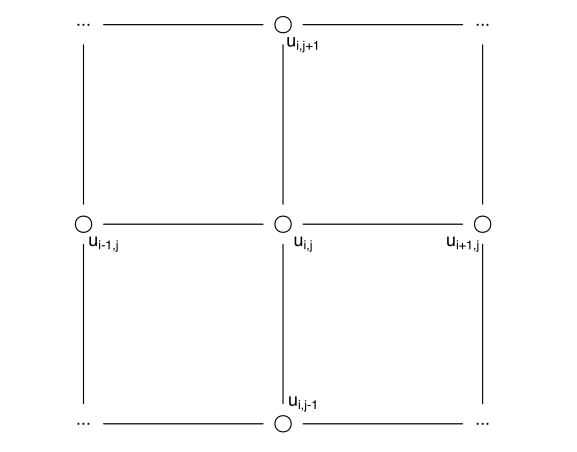
\includegraphics{images/lattice.png}
\caption{lattice 2D regular grid}
\end{figure}

\hypertarget{exploratory}{%
\chapter{Exploratory Analysis}\label{exploratory}}

Data flows out the REST API end point \texttt{*/complete} in a .json format. Data can be filtered out On the basis of the options set in the API endpoint argument body. Some of the options supplied to the API, as in section \ref{APIdocs}, might regard the real estate \texttt{city} interested, \texttt{npages} as the number of pages to scrape, \texttt{type} as the choice between rental of selling market. Since to the analysis extent data should come from the same geographic area API, city and filter parameters are kept permanent (e.g.~Milan rental real estate within ``circonvallazione'' approximated geo-borders). As a consequence a dedicated endpoint \texttt{.thesis} parameter is passed in the argument body. By setting the option equal to to TRUE the API caller requests thesis data. In other words the latter option under the hood secures to specify to the API an already composed query url to be passed to the scraping endppoint, which corresponds to precise zones imposed while searching for advertisemnts on Immobiliare.it. To help figure out the idea behind the operation it can be thought as refreshing everyday the same immobiliare.it url on their website looking for accomodations within a specified zone.
Parameters specified are also npages = 120, leading to to 3000 observations. The \texttt{*} refers to the EC2 public DNS.

\texttt{http://*/complete/120/milano/affitto/.thesis=true}

As a further data source is available a mondgoDB ATLAS cluster which, because of the scheduler, stocks daily .csv information from Milan real estate. Credentials have to be supplied. For run time reasons also related to the bookdown files continuous building the API endpoint is not called and code chunks outputs are cached due to heavy computation. Instead data is extracted from the MongoDB cluster. A summary table of the columns involved is presented with the goal to introduce the reader to API incoming data. Data needs some heavy preprocess steps to get modeled which is briefly covered in the data preparation part in section \ref{prep}. Data coming from the /complete enndpoint has a geo-statistical spatial component and consequently a spatial representation of the dataset is showed. One further plot points out that geographic coordinates are non-linearly related \ref{fig:NonLinearSpatialRel} to the price response variable so dedicated techniques are required. Exploration starts with factor counts evidencing a ``Bilocale'' prevalence which is then compared to other cities. This suggest some critical Milan real estate market demand information and consequently reflections on the offer. Heating and cooling systems, two of the covariates extracted, are grouped and then arranged by descending order prevalence. They both do not display any significative price change but they bring to the surface an important environmental concern. The same is done by highlighting ridges distribution for other two newly engineered covariates. Data displays bimodality in prices distribution for different n-roomed accommodations and the model should take account of the behavior. Then a piece-wise linear regression is fitted for each n-roomed accommodation sub-group whose single predictor is the square meter footage. The analysis emphasize some valuable economic consequences both for investors interested into property expansions and for tenants that are planning to partition single properties into rentable sub-units. The previous analysis brings along a major question which regards the most valuable properties per single square meter surface and a answer based on data is given. Then a further log linear regression setting is proposed to evaluate the impact of some other presumably important covariate. A Tie Fighter plot displays for which coefficient, associated to each dummyied predictor, there are surprisingly high prices compared to the effect of the square meter footage expansion. A partial conclusion is that having 2 or 3 bathrooms truly pays an extra monthly gain, also caused by the number of tentants the accomodations could host. Then missing assessement and imputation takes place. At first is made a brief a revision of missing and randomnes by \citet{Little}, then theory is applied by visualizing missing in combination with heat-map and co-occurrence plot. Combined missing observation test is able to detect whether data is missing because of inner scraping faiilures or simple rarity in data appereance. Then for the observations that passed the test imputation is made through INLA posterior expectation. That is the case of data lost in predictors so the missing covariates ( \emph{condominium} ) are brought into a model as response variable whose this time predictors are explanatory ones. Through a method specified within the INLA function the posterior statistics are computed and then finally imputed in the place of missing ones.

Visualisations are done with ggplot2 in a Tidyverse approach. Maps are done with ggplot2 too and Leaflet, together with its extensions.
A preliminary API data exploratory analysis evidences 34 covariates and 250 rows, which are once again conditioned to the query sent to the API. Immobiliare.it furnishes many information regarding property attributes and estate agency circumstances. Data displays many NA in some of the columns but georeference coordinates, due to the design of scraping functions, are in any case present.

\begin{longtable}{ll}
\toprule
name & ref\\
\midrule
ID & ID of the apartements\\
LAT & latitude coordinate\\
LONG & longitude coordinate\\
LOCATION & the complete address: street name and number\\
CONDOM & the condominium monthly expenses\\
\addlinespace
BUILDAGE & the age in which the building was contructed\\
FLOOR & the property floor\\
INDIVSAPT & indipendent property type versus apartement type\\
LOCALI & specification of the type and number of rooms\\
TPPROP & property type residential or not\\
\addlinespace
STATUS & the actual status of the house, ristrutturato, nuovo, abitabile\\
HEATING & the heating system Cen\_Rad\_Gas (centralizzato a radiatori, alim a gas), Cen\_Rad\_Met,\\
AC & air conditioning hot and cold, Autonomo, freddo/caldo, Centralizzato, freddo/caldo\\
PUB\_DATE & the date of publication of the advertisement\\
CATASTINFO & land registry information\\
\addlinespace
APTCHAR & apartement main characteristics\\
PHOTOSNUM & number of photos displayed in the advertisement\\
AGE & real estate agency name\\
LOWRDPRICE.originalPrice & If the price is lowered it flags the starting price\\
LOWRDPRICE.currentPrice & If the price is lowered it flags the current price\\
\addlinespace
LOWRDPRICE.passedDays & If the price is lowered indicates the days passed since the price has changed\\
LOWRDPRICE.date & If the price is lowered indicates the date the price has changed\\
ENCLASS & the energy class according to the land registers\\
CONTR & the type of contract\\
DISP & if it is still avaiable or already rented\\
\addlinespace
TOTPIANI & the total number of the building floors\\
PAUTO & number of parking box or garages avaibable in the property\\
REVIEW & estate agency review, long chr string\\
HASMULTI & it if has multimedia option, such as 3D house vitualization home experience or videos\\
PRICE & the monthly price <- response\\
\addlinespace
SQFEET & square meters footage\\
NROOM & the number of rooms in the house, and their types\\
TITLE & title of published advertisement\\
\bottomrule
\end{longtable}

\hypertarget{prep}{%
\section{Data preparation}\label{prep}}

Data needs to undergo to many previous cleaning preprocess steps, this is a forced stage since API data comes in human readable format, which is not prepared to be modeled. Cleaning steps mainly regards:

\begin{itemize}
\item
  encoding from UTF-8 to Latin due to Italian characters incorrectly parsed.
\item
  \emph{FLOORS} covariate needs to be separated by its \emph{ASCENSORE} and \emph{ACCDISABILI} components, adding 2 more bivariate covariates.
\item
  \emph{LOCALI} needs to be separated too. 5 category levels drain out: \emph{TOTLOCALI}, \emph{CAMERELETTO}, \emph{ALTRO}, \emph{BAGNO}, \emph{CUCINA}. \emph{NROOM} is a duplicate for \emph{TOTLOCALI}, so it is discarded.
\item
  \emph{APTCHAR} is a list column so that each observation has different categories inside. The preprocess step includes unnesting the list by creating as many bivariate columns as elements in the list. Then new columns flag the existence of the characteristics in the apartment. A slice for the fist APTCHAR observation displays:
\item
  \begin{itemize}
  \tightlist
  \item
    fibra ottica- - - videocitofono- - - impianto di allarme- - - porta blindata- - - reception- - - balcone- - - portiere intera giornata- - - impianto tv centralizzato- - - parzialmente arredato- - - esposizione doppia- -
  \end{itemize}
\end{itemize}

\hypertarget{maps-and-geo-visualisations}{%
\subsection{Maps and Geo-Visualisations}\label{maps-and-geo-visualisations}}

Geographic coordinates can be represented on a map in order to reveal first symptoms of spatial autocorrelation. Observations are spread almost equally throughout the surface even though the response var \emph{PRICE} indicates unsurprisingly that higher prices are nearer to the city center.
The map in figure @ref(fig:leaflet\_visuals) is a leaflet object, which can needs to be overlapped with layers indicating different maps projections. This is interactive in the .html version, and static is proposed in the .pdf output version. The map object takes a input the latitute and longitude coordinates coming from THE API, and they do not need any CRS (Coordinate Reference System) projection since leaflet can accept the data type.

\begin{figure}
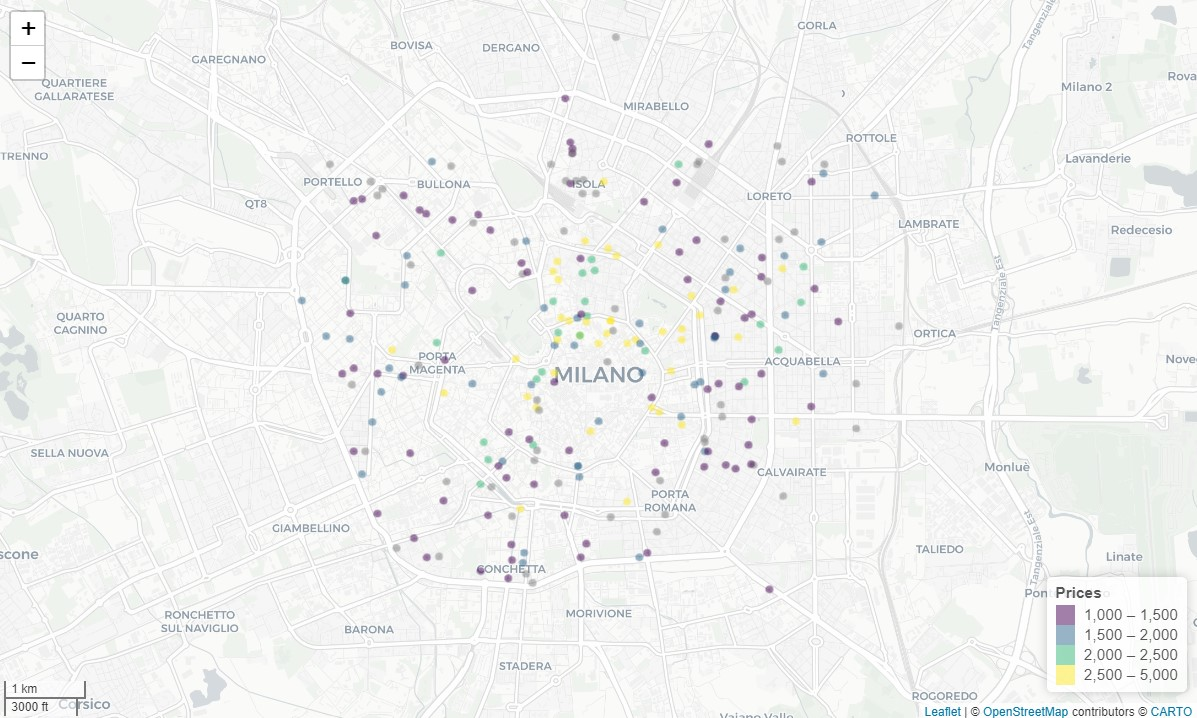
\includegraphics[width=1\linewidth]{images/leaflet_prezzi} \caption{Leaflet Map}\label{fig:LeafletVisuals}
\end{figure}

Predictors, in this case latitude and longitude appear to have nonlinear relationships with the outcome price. The relationship appears to be Gaussian whose mean points to the city center, red dashed line represent latitude and longitude coordinates for the Dome of Milan. Non linearities can be treated with regression splines

\begin{figure}
\centering
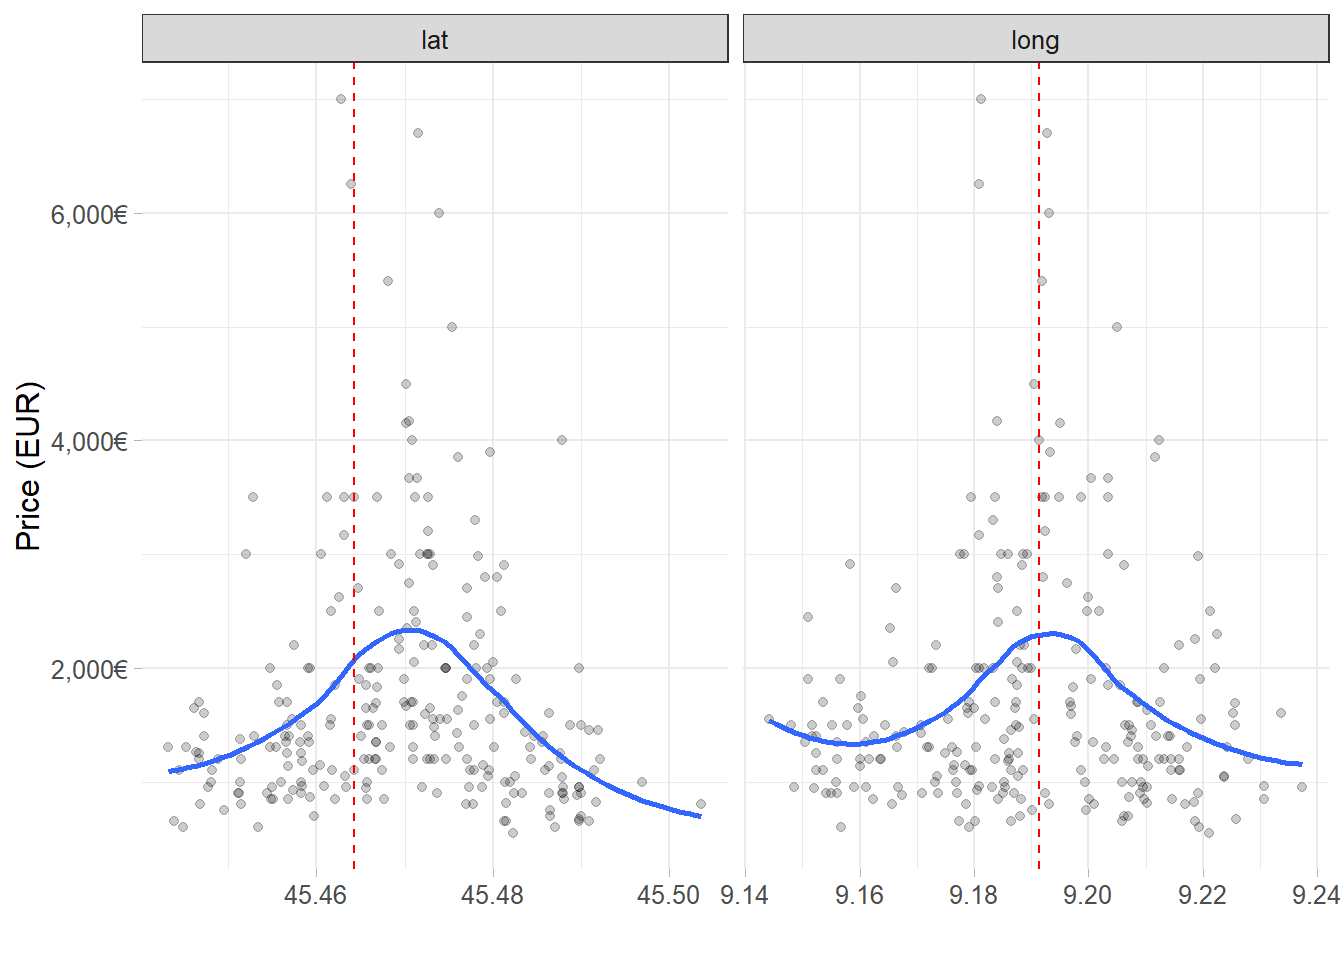
\includegraphics{07-exploratory_files/figure-latex/NonLinearSpatialRel-1.pdf}
\caption{\label{fig:NonLinearSpatialRel}Non Linear Spatial Relationship disclosed}
\end{figure}

\hypertarget{counts-and-first-orientations}{%
\section{Counts and First Orientations}\label{counts-and-first-orientations}}

Arranged Counts for categorical columns can give a sense of the distribution of categories across the dataset suggesting also which predictor to include in the model. The visualization in figure \ref{fig:fctCounts} offers the rearranged factor \emph{TOTLOCALI}.
Bilocali are the most common option for rent, then trilocali comes after. The intuition behind suggests that Milan rental market is oriented to ``lighter'' accommodations in terms of space and squarefootage. This should comes natural since Milan is both a vivid study and working area, so short stayings are warmly welcomed.

\begin{figure}
\centering
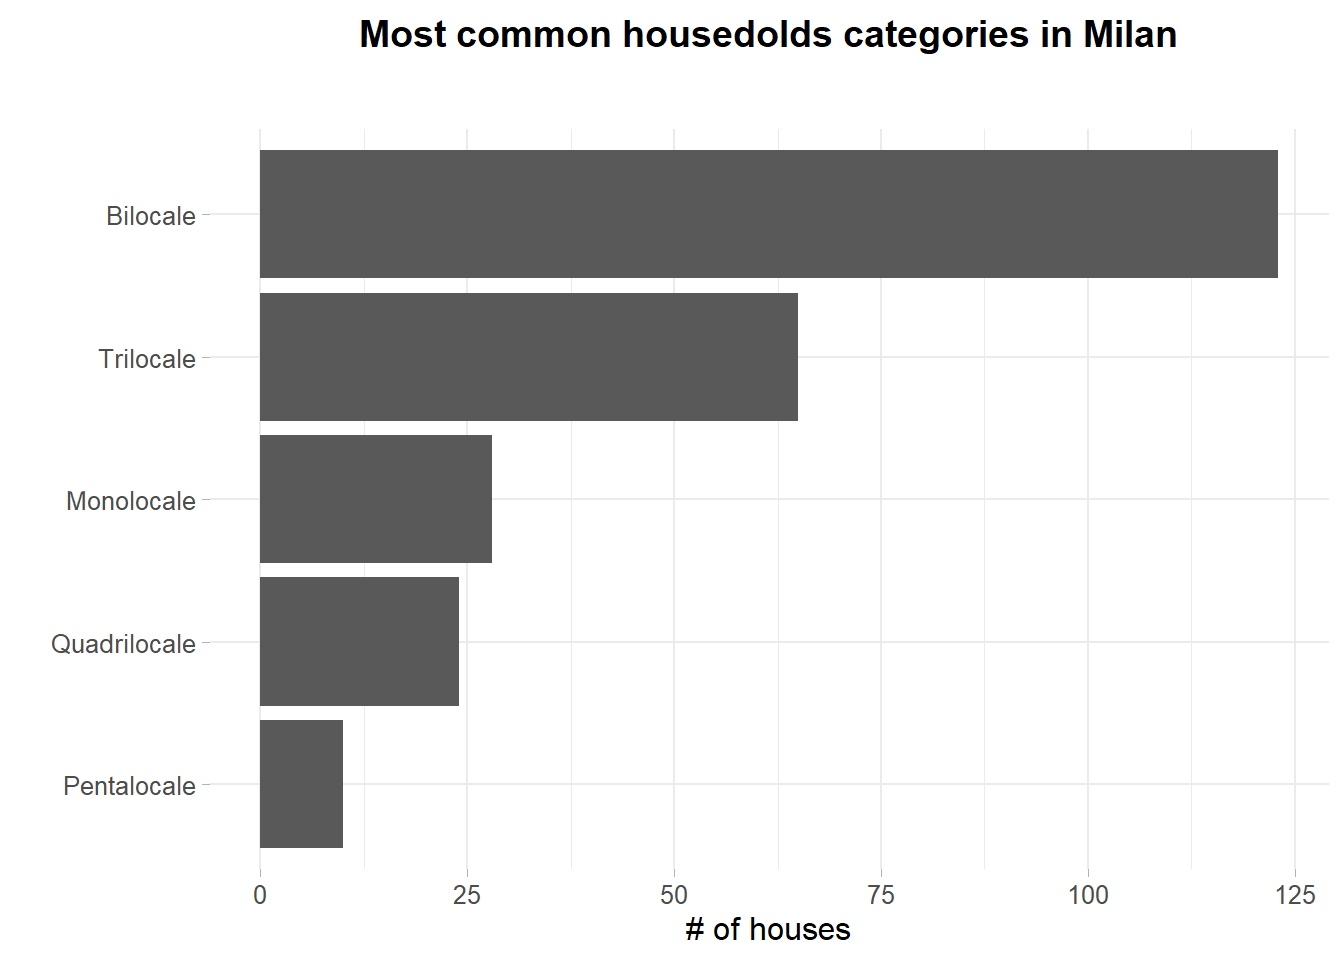
\includegraphics{07-exploratory_files/figure-latex/fctCounts-1.pdf}
\caption{\label{fig:fctCounts}Most common housedolds categories}
\end{figure}

Two of the most requested features for comfort and livability in rents are the heating/cooling systems installed. Moreover rental market demand, regardless of the rent duration, strives for a ready-to-accomodate offer to meet clients needs. In this sense accomodation coming with the newest and most techonological systems are naturally preferred with respect the contrary.
x-axis in figure \ref{fig:PricePerAc} represents log\_10 price for both of the two plots. Logarithmic scale is needed to smooth distributions and the resulting price interpretation have to considered into relative percent changes. Furthermore factors are reordered with respect to decreasing price.\\
y-axis are the different level for the categorical variables recoded from the original data due to simplify lables and to hold plot dimension. Moreover counts per level are expressed between brackets close to their respective factor.
The top plot displays the most prevalent heating systems categories, among which the most prevalent is ``Cen\_Rad\_Met'' by far. This fact is extremely important since metano is a green energy source and if the adoption is wide spread and pipelines are well organized than it brings enormous benefit to the city. As a consequence one major concern regards that for many years policies have been oriented to reduce vehicles emission (euro1 euro2\ldots) instead of focusing on house emissions. This was also a consequence of the lack of house data especially in rural areas. According to data there are still a 15\% portion of houses powered by oil fired.
Then in bottom plot Jittering is then applied to point out the number of outliers outside the IQR (Inter Quantile Range) .25 and their impact on the distribution. A first conclusion is that outliers are mainly located in autonomous systems, which leads of course to believe that the most expensive houses are heated by autonomoius heating systems. Indedd in any case this fact that does not affect monthly price. The overlapping IQR signifies that the covariates levels do not impact the response variable.

\begin{figure}
\centering
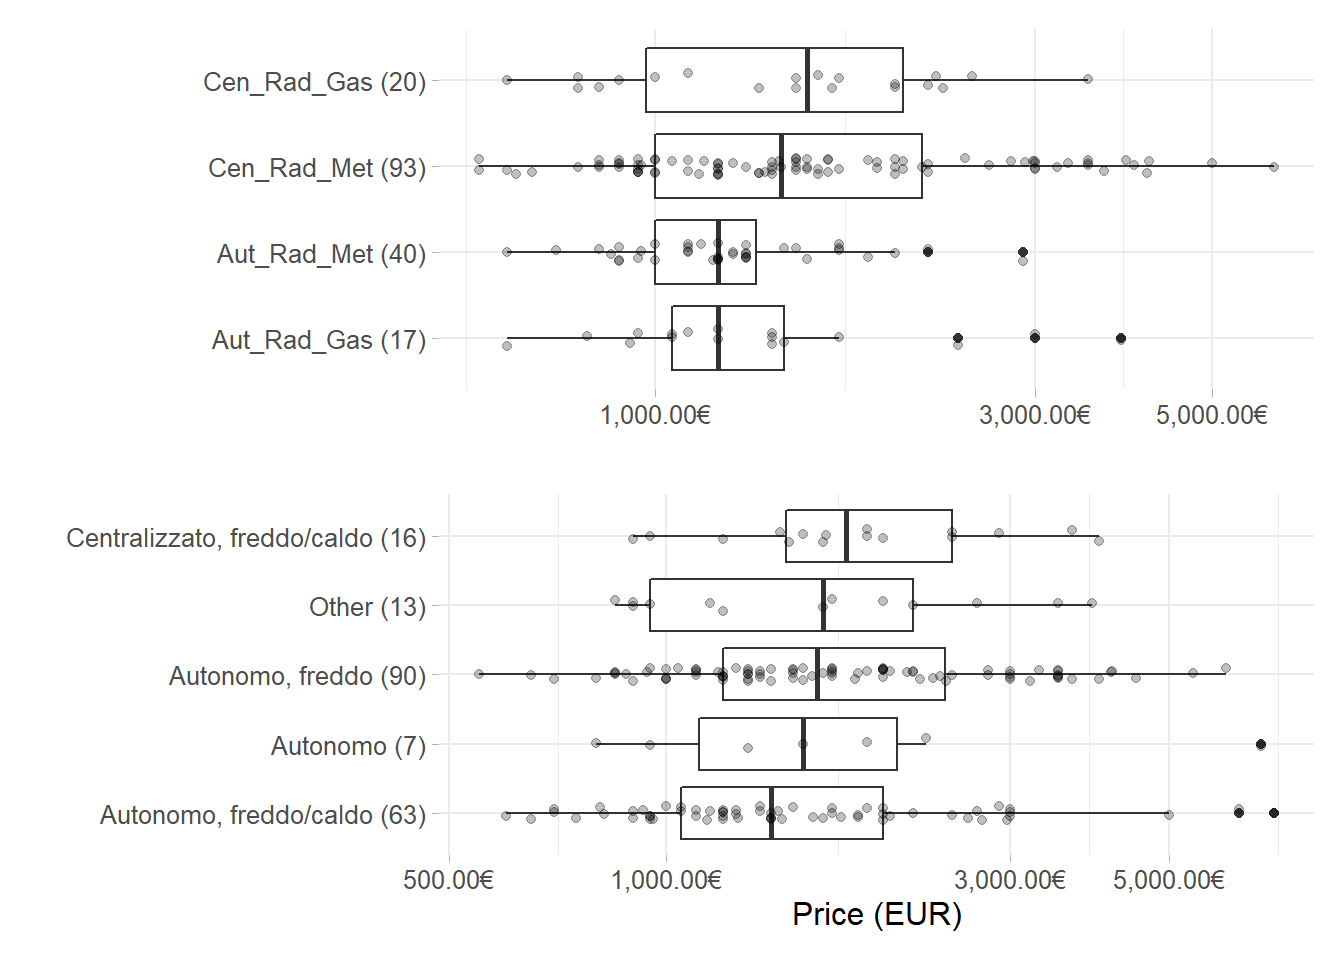
\includegraphics{07-exploratory_files/figure-latex/PricePerAc-1.pdf}
\caption{\label{fig:PricePerAc}Log Monthly Price per Heating/Cooling system?}
\end{figure}

this visualization intersects allows to discover bimodality in the response variable. Log scales was needed since they are all veru skewd and log scale then is needed also in the model.

(qui ci puoi mettere a confronto per variabile bianria, così vedi cosa includere nel modello esempio sotto dove commentato, )

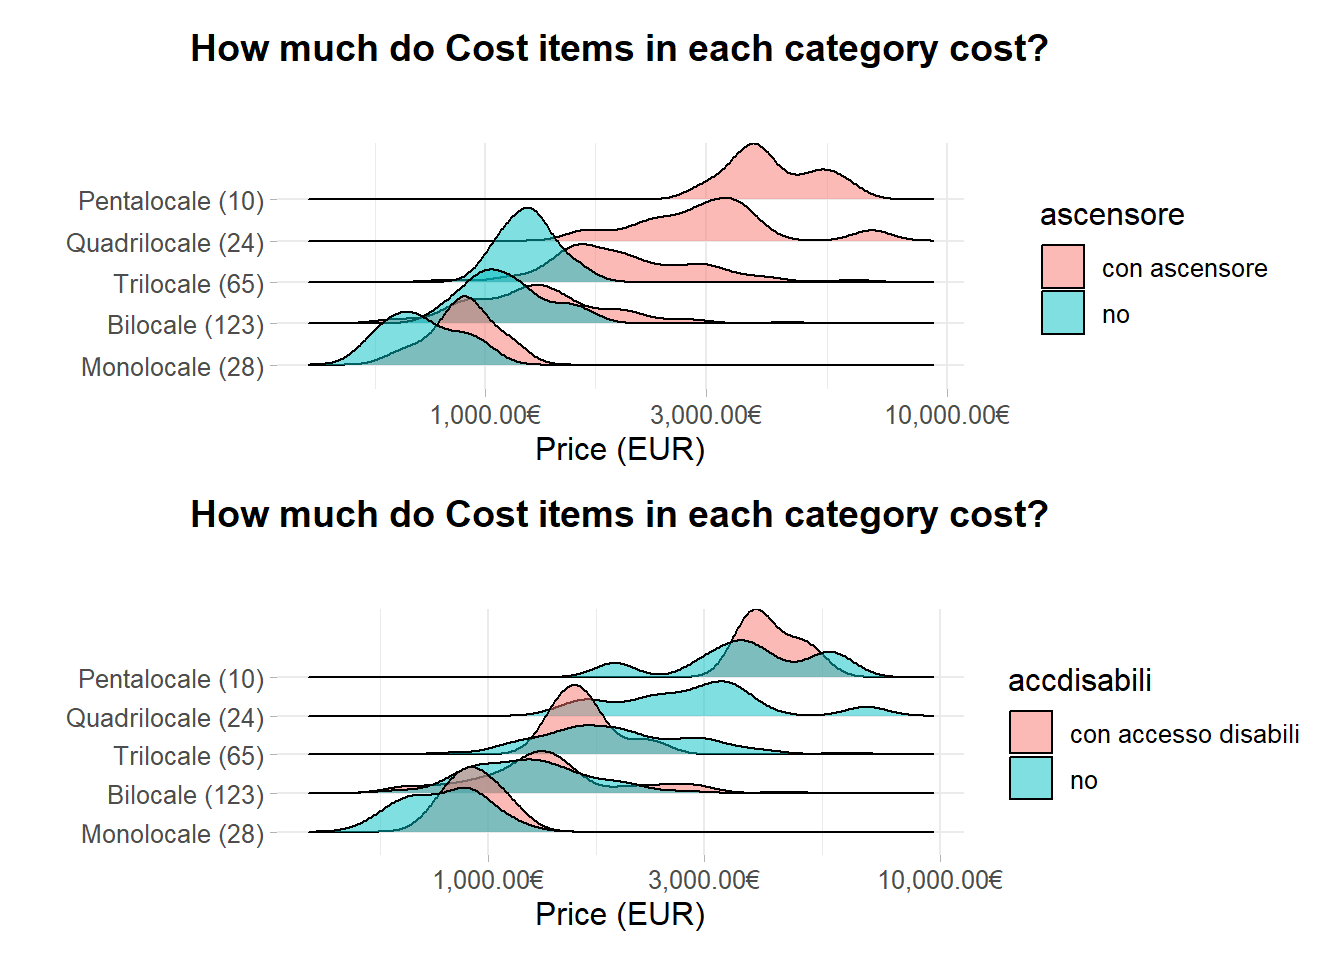
\includegraphics{07-exploratory_files/figure-latex/unnamed-chunk-1-1.pdf}

What it might be really relevant to research is how monthly prices change with respect to house square footage for each house configuration. The idea is to asses how much adding a further square meter affetcs the monthly price for each n-roomed flat.
One implication is how the property should be developed in order to request a greater amount of money per month. As an example in a situation in which the household has to lot its property into different sub units he can be helped to decide the most proficient choice in economic terms by setting ex ante the square footage extensions for each of the sub-properties.
A further implication can regard economic convenience to enlarge new property acquisitions under the expectation to broadened the square footage (construction firms). Some of the potential enlargements are economically justified, some of the other are not.
The plot \ref{fig:GlmPriceSq} has two continuous variables for x (price) and y (sqfeet) axis, the latter is log 10 scaled due to smoothness reasons. Coloration discretizes points for the each \(j\) household rooms totlocali. A sort of overlapping piece-wise linear regression (log-linear due to transformation) is fitted on each totlocali group, whose response variable is price and whose only predictor is the square footage surface (i.e.~\(\log_{10}(\mathbf{price_j}) \sim +\beta_{0,j}+\beta_{1,j}\mathbf{sqfeet_j}\)). Five different regression models are proposed in the top left. The interesting part regards the models slopes \(\hat\beta_{1,j}\). The highest corresponds to ``Monolocale'' for which the enlargement of a 10 square meters in surface enriches the apartment of a 0.1819524\% monthly price addition. Almost the same is witnessed in ``Bilocale'' for which a 10 square meters extension gains a 0.1194379\% value. One more major thing to notice is the ``ensamble'' regression line obtained as the interpolation of the 5 plotted ones. The line suggests a clear slope descending pattern (logarithmic trend) from Pentalocale and beyond whose assumption is strengthened by looking at the decreasing trend in the \(\hat\beta_1\) predictor slopes coefficients. Furthermore investing into an extension for ``Quadrilocale'' and ``Trilocale'' is \emph{coeteris paribus} an interchangeable economic choice.

\begin{figure}
\centering
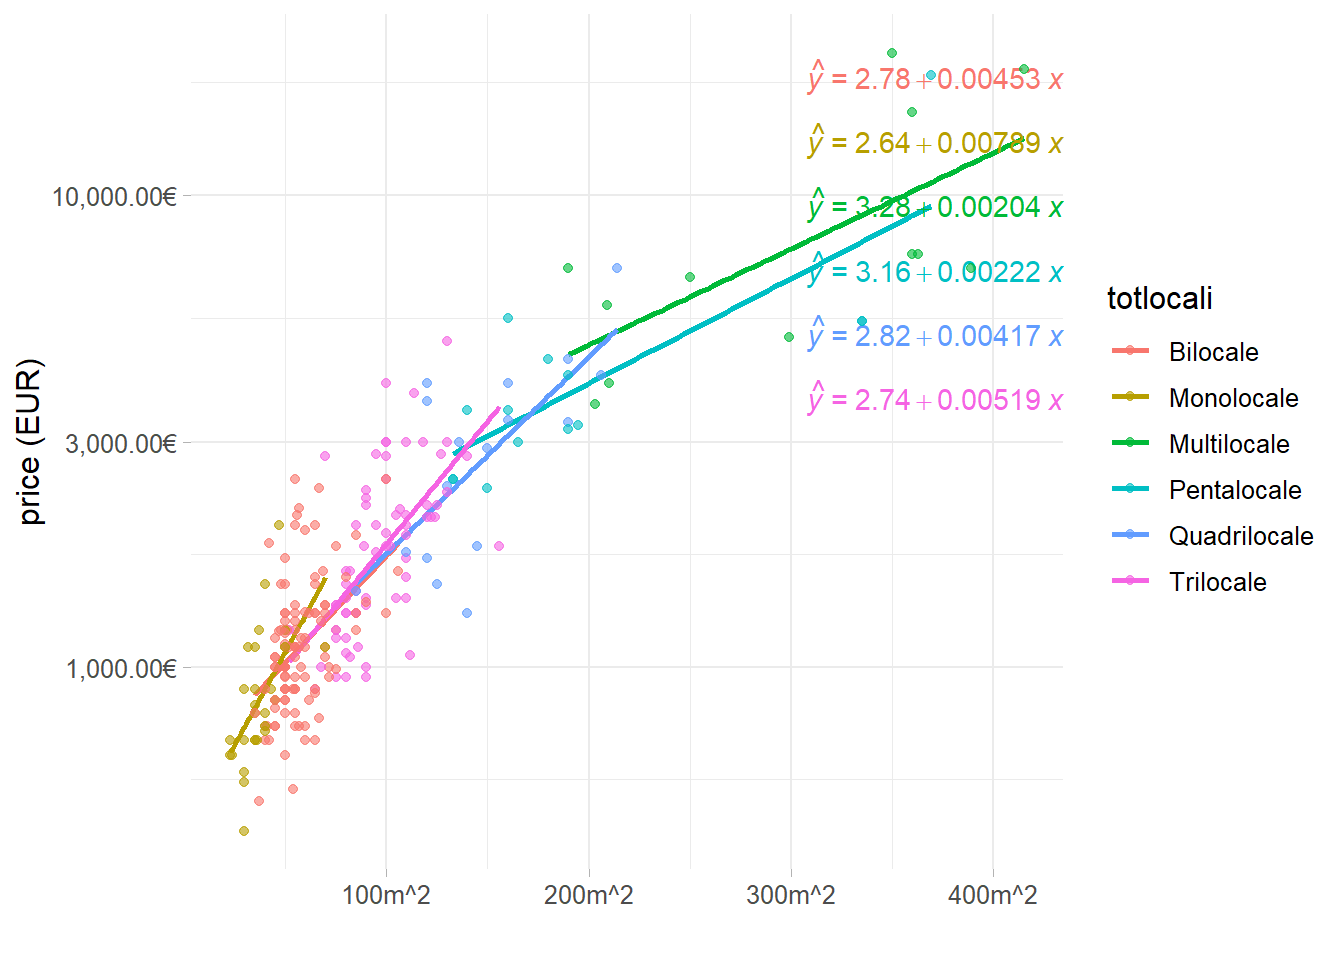
\includegraphics{07-exploratory_files/figure-latex/GlmPriceSq-1.pdf}
\caption{\label{fig:GlmPriceSq}Monthly Prices change wrt square meters footage in different n-roomed apt}
\end{figure}

In table (\ldots) resides the answer to the question ``which are the most profitable properties per month in terms of the price per square meter footage ratio''. The covariate floor together with the totpiani are not part of the model, indeed they can explain the importance and the height of the building justifying extraordinary prices. The first 4 observations are unsurprisingly ``Bilocale'', the spatial column location, not a regressor, can lend a hand to acknowledge that the street addresses point to very central and popular zones. The zones are, first City Life, second Brera and third Moscova, proving that in modeling real estate rents the spatial component is fundamental , even more in Milan.

\begin{tabular}{llrrllr}
\toprule
location & totlocali & price & sqfeet & floor & totpiani & abs\_price\\
\midrule
viale cassiodoro 28 & Bilocale & 1750 & 30 & 9 piano & 10 piani & 58.33333\\
via della spiga 23 & Bilocale & 2750 & 55 & 2 piano & 4 piani & 50.00000\\
corso giuseppe garibaldi 95 & Bilocale & 2700 & 56 & 2 piano & 5 piani & 48.21429\\
piazza san babila C.A. & Bilocale & 1833 & 42 & 4 piano & 4 piani & 43.64286\\
ottimo stato piano terra, C.A. & Trilocale & 3000 & 80 & Piano terra & 3 piani & 37.50000\\
\addlinespace
via federico confalonieri 5 & Monolocale & 750 & 20 & 1 piano & 3 piani & 37.50000\\
\bottomrule
\end{tabular}

Then as a further point it might be important to investigate a linear model whose response is price and whose covariates are the newly created abs\_price and some other presumably important ones e.g.~floor, bagno, totpiani. The model fitted is \texttt{log2(price)\ \textasciitilde{}\ log2(abs\_price)\ +\ bagno\ +\ floor\ +\ totpiani}.
The plot in figure \ref{fig:TieFighterPlot} has the purpose to demonstrate how monthly price is affected by covariates conditioned to their respective square meter footage. The interpretation of the plot starts by fixing a focus point on 0, which is the null effect highlighted by the red dashed line. Then the second focus is on house surface effect (i.e.~House Surface (doubling) in the plot, the term log2(abs\_price) has been converted to more familiar House Surface (doubling)), which contributes to increase the price of an estimated coefficient of \(\approx .6\) for each doubling of the square meter footage. Then what it can be noticed with respect to the two focus points are the unusual effects provoked by the other predictors t the right of the house surface effect and to the far left below 0. ``2 and 3 bagni'' are unusually expensive with respect to the square meter footage increment, on the other hand" al piano rialzato" and ``al piano terra'' are undervalued with respect to their surface. The fact that 2 and 3 bathrooms can guarantee a monthly extra check is probably caused to a minimum rent plateau requested for each occupant. the number of bathrooms are a proxy to both house extension since normally for each sleeping room there also exist at least 1 bathroom as well as prestigious houses dispose of more than 1 toilette services. So the more are the occupants regardless of the square meter footage dedicated to them, the more the house monthly returns,

it can be noticed is that ultimo piano, otgether with 2 abagni ad 3 bagni are unusually expensive with respect to their proper square meter footage. On the other hand the piano rialzato and piano terra are unusually undervalued given their surface.\\
In other words the to help with the interpretation. The fact that 2 and 3 bathrooms can guarantee a monthly extra check is probably caused to a minimum rent plateau requested for each occupant. So the more are the occupants regardless of the square meter footage dedicated to them, the more the house returns. The conclusion

\begin{figure}
\centering
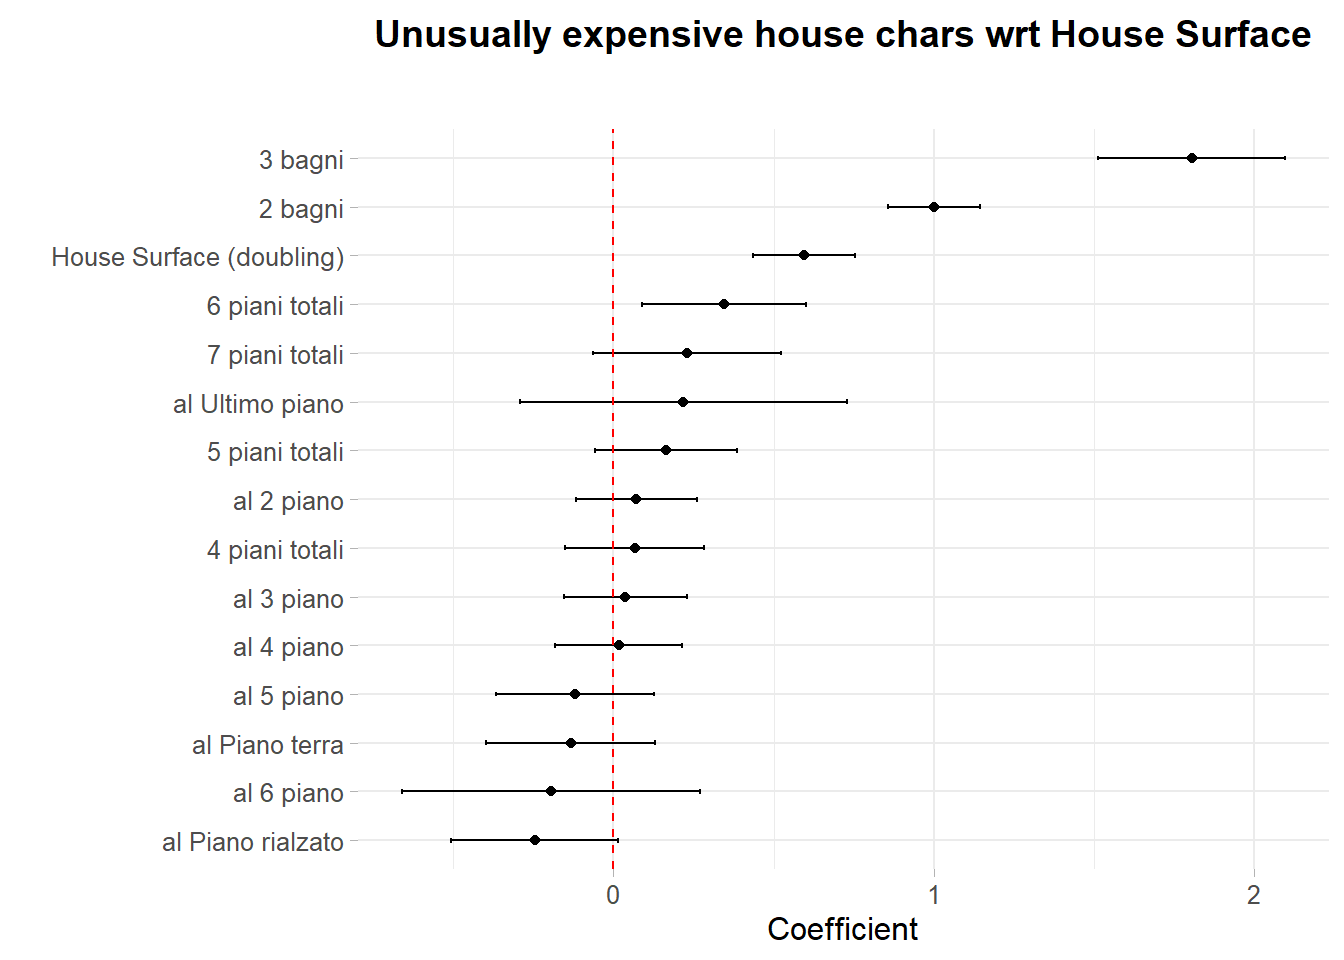
\includegraphics{07-exploratory_files/figure-latex/TieFighterPlot-1.pdf}
\caption{\label{fig:TieFighterPlot}Coefficient Tie fighter plot for the linear model: log2(price) \textasciitilde{} log2(abs\_price) + condom + other\_colors}
\end{figure}

(se vuoi dire qualcosa sul condominio)

\hypertarget{missing-assessement-and-imputation}{%
\section{Missing Assessement and Imputation}\label{missing-assessement-and-imputation}}

As already pointed out some data might be lost since immobiliare provides the information that in turn are pre filled by estate agencies or privates through standard document formats. Some of the missing can be reverse engineered by other information in the web pages e.g.~given the street address it is possible to trace back the lat and long coordinates. Some other information can be encountered in .json files hidden inside each of the single web pages.
The approach followed in this part is to prune redundant data and rare predictors trying to limit the dimensionality of the dataset.

\hypertarget{missing-assessement}{%
\subsection{Missing assessement}\label{missing-assessement}}

The first problem to assess is why information are missing. As already pointed out in the preliminary part as well as in section \ref{ContentArchitecture} many of the presumably important covariates (i.e.~price lat, long, title ,id \ldots) undergo to a sequence of forced step inside scraping functions with the aim to avoid to be lost. If at the end of the sequence covariates are still missing, the correspondent observation is not considered and it is left out of the resulting scraped dataset. The choice originates from empirical missing patterns suggesting that when important information are missing then the rest of the covariates are more likely to be missing to, as a consequence the observation should be discarded.
The missing profile is crucial since it can also raise suspicion on the scraping failures. By Taking advantage of the missing pattern in observations the maintainer can directly identify the problem and derivatives and immediately debug the error. In order to identify if the nature of the pattern a revision of missing and randomness is introduced by \citet{Little}.
Missing can be devided into 3 categories:

\begin{itemize}
\tightlist
\item
  \emph{MCAR} (missing completely at random) likelihood of missing is equal for all the information, in other words missing data are one idependetn for the other.
\item
  \emph{MAR} (missing at random) likelihood of missing is not equal.
\item
  \emph{NMAR} (not missing at random) data that is missing due to a specific cause, scarping can be the cause.
\end{itemize}

MNAR is often the case of daily monitoring clinical studies \citep{Kuhn}, where patient might drop out the experiment because of death and so all the relating data starting from the death time +1 are lost.
To identify the pattern a \emph{heat map} plot \ref{fig:Heatmap} clarifies the idea:

\begin{figure}
\centering
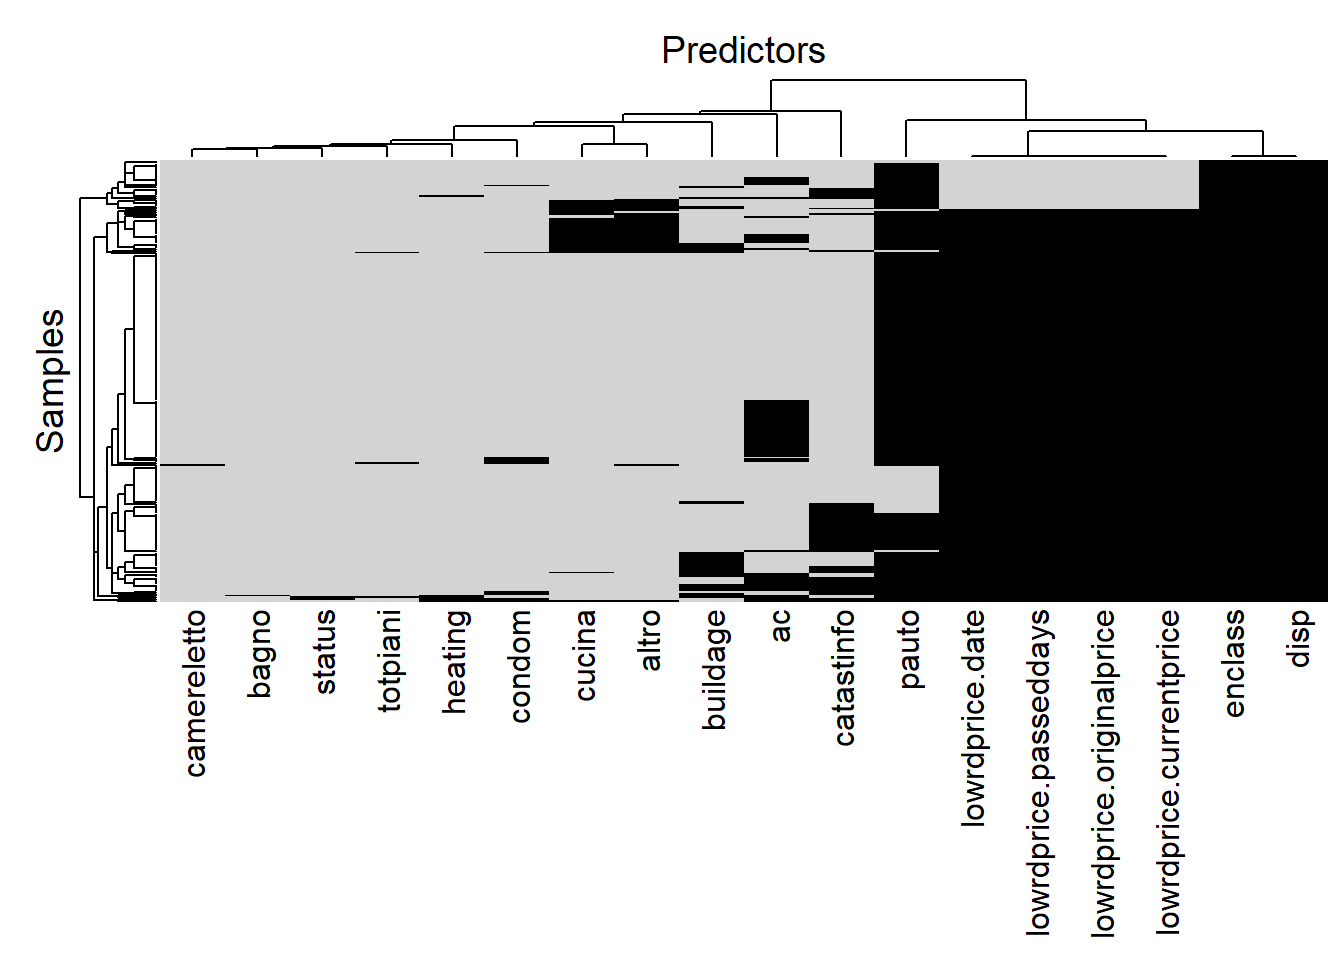
\includegraphics{07-exploratory_files/figure-latex/Heatmap-1.pdf}
\caption{\label{fig:Heatmap}Missingness Heatmap plot}
\end{figure}

Looking at the top of the heat map plot, right under the ``Predictor'' label, the first tree split divides predictors into two sub-groups. The left branch considers from \emph{TOTPIANI} to \emph{CATASTINFO} and there are no evident patterns. Then missingness can be traced back to MAR. Imputation needs to be applied up to \emph{CONDOM} included, the others are discarded due to rarity: i.e.~\emph{BUILDAGE}: 14\% missing, \emph{CATASTINFO}: 21\% and \emph{AC}: 24\%. Moreover \emph{CUCINA} and \emph{ALTRO} are generated as ``childred'' of the original \emph{LOCALI} variable, so it should not surprise that their missing behavior is similar ,whose prevalence is respectively 13\% and 14\%, for that reason are discarded.
In the far right hand side \emph{ENCLASS} and \emph{DISP} data are completely missing and a pattern seems to be found. The most obvious reason is a scraping fail in capturing data. Further inspection of the API scraping functions focused on the two covariates is strongly advised. From \emph{LOWRDPRICE.} covariates gorup class it seems to be witnessing a missing underlining pattern NMAR which is clearer by looking at the co\_occurrence plot in figure \ref{fig:cooccurrence}. Co-occurrence analysis might suggest frequency of missing predictor in combination and \emph{LOWRDPRICE.} class covariates are displaying this type of behavior. \emph{PAUTO} is missing in the place where \emph{LOWRDPRICE.} class covariates are missing, but this is not happening for the opposite, leading to the conclusion that \emph{PAUTO} should be treated as a rare covariate MAR, therefore \emph{PAUTO} is dropped.
After some further investigation on \emph{LOWRDPRICE.}, the group class flags when the \emph{PRICE} covariate is effectively decreased and this is unusual. That is solved by grouping the covariate's information and to encode it as a two levels categorical covariate if lowered or not. Further methods to feature engineer the \emph{LOWRDPRICE.} class covariates can be with techniques typical of profile data, further references are on \citet{Kuhn}.

\begin{figure}
\centering
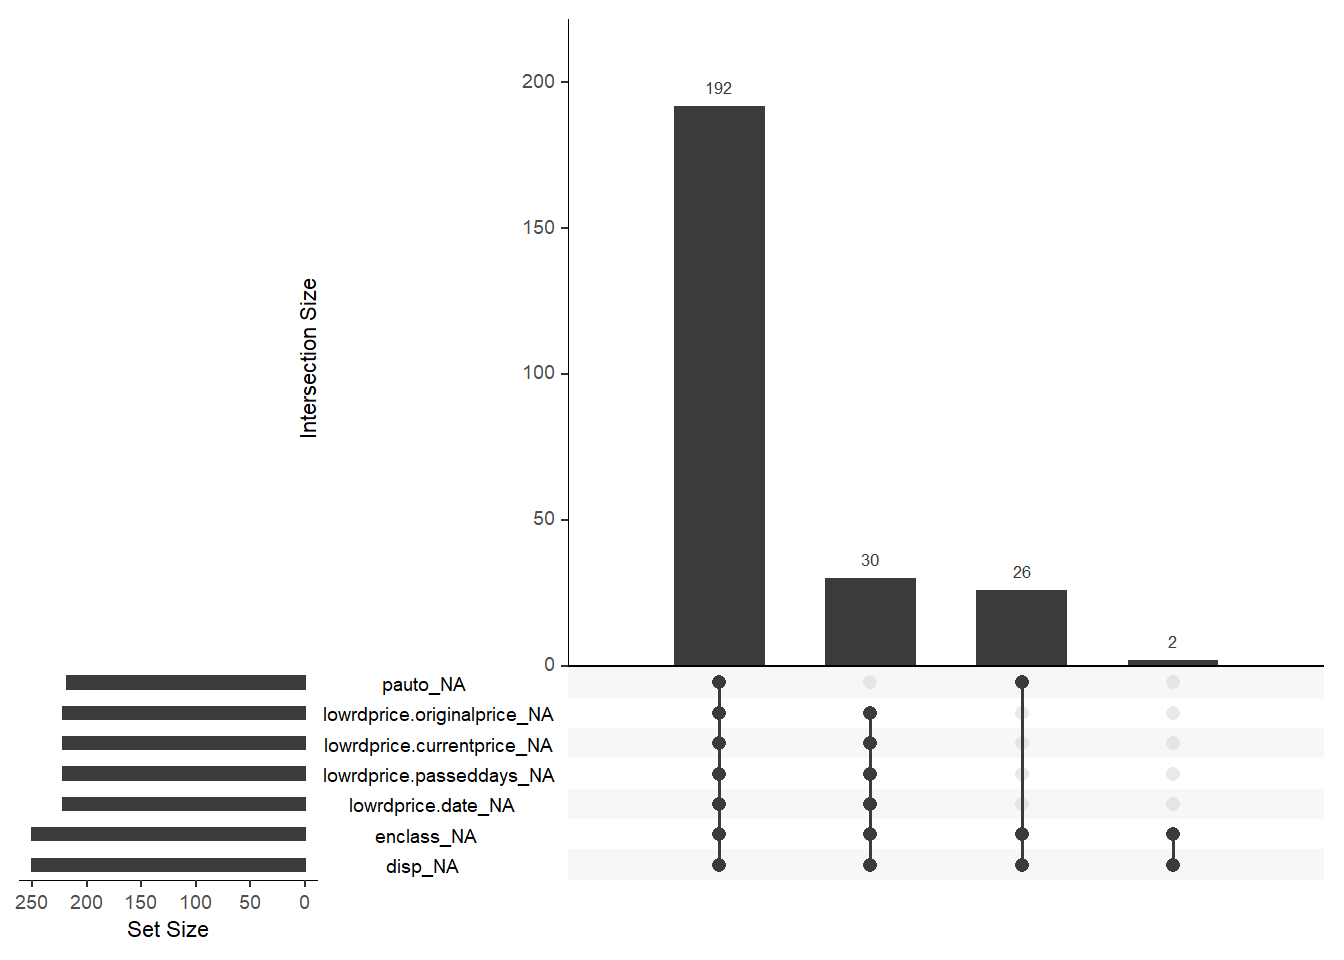
\includegraphics{07-exploratory_files/figure-latex/cooccurrence-1.pdf}
\caption{\label{fig:cooccurrence}Missingness co-occurrence plot}
\end{figure}

\hypertarget{covariates-imputation}{%
\subsection{Covariates Imputation}\label{covariates-imputation}}

A relatively simple approach to front missingness is to build a regression model to explain the covariates that have some missing and plug-back-in the respective estimates (e.g.~posterior means) from their predictive distributions \citet{Little}. This approach is fast and easy to implement in most of the cases, but it ignores the uncertainty behind the imputed values \citep{Bayesian_INLA_Rubio}. However it has the benefit to be a more than a reasonable choice with respect to the number of computation required, especially with INLA and in a spatial setting. That makes it the first choice method to follow since imputation regards also a small portion of data and predictors. At first it is considered the predictor \emph{condominium} for which some observation are missing. Indices are:

\begin{verbatim}
##  [1]  19  74  77  90  99 113 116 120 179 249
\end{verbatim}

A model is fitted based on missing data for which the response var is condominium and predictors are other important explanatory ones, i.e.\texttt{condom\ \textasciitilde{}\ 1\ +\ sqfeet\ +\ totlocali\ +\ floor\ +\ heating\ +\ ascensore}. In addition to the formula in the inla function a further specification has to be provided with the command \texttt{compute\ =\ TRUE} in the argument control.predictor. The command \texttt{compute} estimates the posterior means of the predictive distribution in the response variable for the missing points. The estimated posetior mean quantities are then imputeda are in table @red(tab:CondomImputation)

\begin{tabular}{lrr}
\toprule
  & mean & sd\\
\midrule
fitted.Predictor.019 & 198.11095 & 19.67085\\
fitted.Predictor.074 & 162.96544 & 13.29456\\
fitted.Predictor.077 & 99.38197 & 32.34108\\
fitted.Predictor.090 & 331.73519 & 33.05035\\
fitted.Predictor.099 & 170.54068 & 12.30267\\
\addlinespace
fitted.Predictor.113 & 196.61593 & 15.86545\\
fitted.Predictor.116 & 108.40482 & 20.79689\\
fitted.Predictor.120 & 162.86977 & 25.61622\\
fitted.Predictor.179 & 165.03632 & 20.53485\\
fitted.Predictor.249 & 117.24234 & 30.80290\\
\bottomrule
\end{tabular}

A further method for imputation has been designed by \emph{Gómez-Rubio, Cameletti, and Blangiardo 2019) miss lit} by adding a sub-model for the imputations to the final model through the inla function. This is directly handled inside the predictor formula adding a parameter in the latent field. However the approach makes the model more complex with a further layer of uncertainty to handle.
At first the additive regression model with all the covariates is called including the covariates with missing values. The response variable \emph{PRICE} displays no missing values and the model fitted is:

\hypertarget{model-specification}{%
\section{Model Specification}\label{model-specification}}

\hypertarget{mesh-building}{%
\section{Mesh building}\label{mesh-building}}

\emph{PARAFRASARE}
The SPDE approach approximates the continuous Gaussian field \(w_{i}\) as a discrete Gaussian Markov random field by means of a finite basis function defined on a triangulated mesh of the region of study. The spatial surface can be interpolated performing this approximation with the inla.mesh.2d() function of the R-INLA package. This function creates a Constrained Refined Delaunay Triangulation (CRDT) over the study region, that will be simply referred to as the mesh. Mesh should be intended as a trade off between the accuracy of the GMRF surface representation and the computational cost, in other words the more are the vertices, the finer is the GF approximation, leading to a computational funnel.

\begin{figure}
\centering
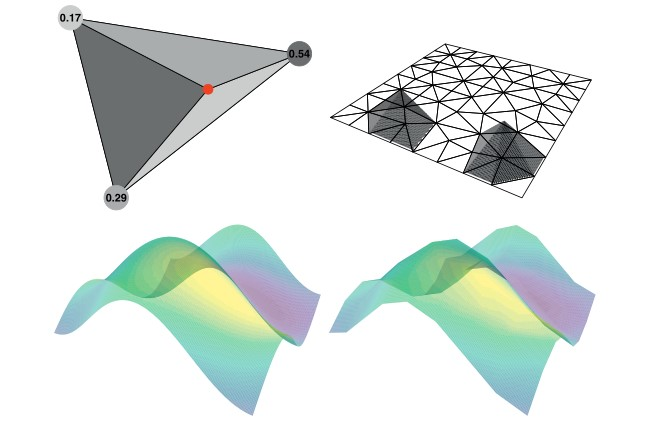
\includegraphics{images/triangle.jpg}
\caption{Traingularization intuition, \citet{Krainski-Rubio} source}
\end{figure}

Arguments can tune triangularization through inla.mesh.2d() :

\begin{itemize}
\tightlist
\item
  \texttt{loc}:location coordinates that are used as initial mesh vertices
\item
  \texttt{boundary}:object describing the boundary of the domain,
\item
  \texttt{offset}: argument is a numeric value (or a length two vector) and it is used
  to set the automatic extension distance. If positive, it is the extension distance
  in the same scale units. If negative, it is interpreted as a factor relative to the
  approximate data diameter; i.e., a value of -0.10 (the default) will add a 10\%
  of the data diameter as outer extension.
\item
  \texttt{cutoff}: points at a closer distance than the supplied value are replaced by a single vertex. Hence, it avoids small triangles
\item
  \texttt{max.edge}: A good mesh needs to have triangles as regular as possible in size and shape.
\item
  \texttt{min.angle}argument (which can be scalar or length two vector) can be used to specify the minimum internal angles of the triangles in the inner domain and the outer extension
\end{itemize}

A convex hull is a polygon of triangles out of the domain area, in other words the extension made to avoid the boundary effect. All meshes in Figure 2.12 have been made to have a convex hull boundary. If borders are available are generally preferred, so non convex hull meshes are avoided.

\hypertarget{shinyapp-for-mesh-assessment}{%
\subsection{Shinyapp for mesh assessment}\label{shinyapp-for-mesh-assessment}}

INLA includes a Shiny (Chang et al., 2018) application that can be used to tune the mesh params interactively

The mesh builder has a number of options to define the mesh on the left side. These include options to be passed to functions inla.nonconvex.hull() and inla.mesh.2d() and the resulting mesh displayed on the right part.

\hypertarget{building-spde-model-on-mesh}{%
\subsection{BUilding SPDE model on mesh}\label{building-spde-model-on-mesh}}

\hypertarget{spatial-kriging-prediction}{%
\section{Spatial Kriging (Prediction)}\label{spatial-kriging-prediction}}

QUI INCERTEZZE

\hypertarget{modelspec}{%
\chapter{Model Selection \& Fitting}\label{modelspec}}

\hypertarget{model-criticism}{%
\section{Model Criticism}\label{model-criticism}}

evaluation of the variables to include in the mode,, assumptions of the model i.e.~exchangeablity and independence prior distribution to assign to parameters and hyper parameters.

\hypertarget{spatial-kriging-1}{%
\section{Spatial Kriging}\label{spatial-kriging-1}}

\hypertarget{model-checking-1}{%
\section{Model Checking}\label{model-checking-1}}

if (models \textgreater{} 2)\{

\begin{verbatim}
## Model Selection




  IDEA: proporre due modelli uno più interepretabile con distribuzione normale, e un ò'altro con sempre exponential family ma con Gamma distribution function, ora vedo se riesco a fare tutto. dovrei sacrificare applicazione.
\end{verbatim}

\}

\hypertarget{application}{%
\chapter{Shiny Application}\label{application}}

with UI build with free tool for front end design ion shiny \href{https://fomantic-ui.com/}{fomantic-ui}. prendi shiny app e rifai interface. in questo blog vedi Hacaton tirato e vincitori \href{https://blog.rstudio.com/2020/11/10/the-appsilon-shiny-semantic-pocontest/}{blog}.

Senno app paula moraga che ha già simil modello dentro,

senno flexdashboard paula moraga.

\href{https://demo.appsilon.ai/apps/polluter/}{this inspiration}

\hypertarget{appendix}{%
\chapter*{Appendix}\label{appendix}}
\addcontentsline{toc}{chapter}{Appendix}

\hypertarget{gp-basics}{%
\section{GP basics}\label{gp-basics}}

\href{https://www.youtube.com/watch?v=4vGiHC35j9s\&t=164s}{Nando de Freitas 1}

\href{https://www.youtube.com/watch?v=MfHKW5z-OOA}{Nando de Freitas 2}

lets say there are a cloud of points represented by two variables x1 and x2. the cloud of points describes a realization of this two variable i.e.~height and weight and then you just plot it , you might get measurement like that,

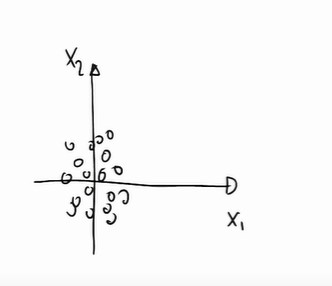
\includegraphics{appendix_images/gp_base_1.jpg}
or:

each circle is a mesuduraments. now when we use multivariate gaussian we fit gaussian to data, the process of learning is to fit a gaussian to data, the ultimate goal is to describe the data, the smartest gaussian in the first image is to center the mean in the 0 and the draw a cricle containin all the other observation. Instaed for the second image it is still centering the mean in 0 but now it is an ellipse describing the variability, the size of the elipse descrube the variability of the data.
the center is a vector \(\mu_{i}\) that it is beacuse we have two components \(x_1\) and \(x_2\) whhose mean is 0 for each of the other. This is true for all the observation which have two coordinates too \(x_1\) and \(x_2\). in vector notations we have for the mean:

\[
\boldsymbol{\mu}=\left[\begin{array}{ll}
\mu_{x_1} \\
\mu_{x_2}
\end{array}\right]
\]

for each of the points, e.g.~for point 1:

\[
\mathbf{x_1}=\left[\begin{array}{ll}
x_1 \\
x_2
\end{array}\right]
\]

the can be neagtive positive, the Real numbers, usually we have \(\mathbb{R}^{2}\) extending from - infinity to + infinity, to the power of two because we have 2 dimensions, a Real plane.

any point is gaussian distributed when with mean .. an variance.
how we explain covariance, thorugh \emph{correlation.}
we do it by correlation with its noraml forms. the covariance is the term that goes insisde the matrices in the upper right of the matrxi we have the expectation of \(x_1\) times \(x_2\), like \(\mathbb{E}(x_1 \cdot x_2)\), where the extactation in the gaussian case is the mean which is 0, so the corresponding values is 0.
the covariance essentially is the dot product \href{https://mathinsight.org/dot_product_matrix_notation}{ref dot product} of \(x_1\) and \(x_2\) variable, so what happens when you take the dot product of vectors,
if for example you take a vector that looks like 1 and 0 and you take the dot product of one other vecto 1 and 0, so that:

\[
\left[\begin{array}{ll}
1 \\
0
\end{array}\right]\left[\begin{array}{ll}
1 & 0 \\
\end{array}\right] = 1
\]
You will end up with 1, recall dot productm first element first vcetor times first element second vectro and second element first vector times second element secon vector. So identical vector will get a high dot product value leading to a high similarity measure. Dot product can be indeded as a similarity measure.
\ldots{} But if you take two different vector as 1 0 and 0 1 then:

\[
\left[\begin{array}{ll}
1 \\
0
\end{array}\right]\left[\begin{array}{ll}
0 & 1 \\
\end{array}\right] = 0
\]

This time the multiplication leads to 0 value, as a matter of fact they are different. They are no similar.
IF two points are closed the dot product will be high in 2D. What the covariance should be? if variances are assumed to be 1 then in this case i qould expect to be 0, i.e.~covariance matrix is:

\[
\left[\begin{array}{ll}
1 & 0 \\
0 & 1
\end{array}\right] = \mathbf{cov_{plot1}}(x_1,x_2)
\]

because I can picka poin tin two pointa in this cloud. Suppose i increase x1 then my chance of getting a x2 point that is positive or negative is the samee, knowing somthin about x1 give nothign about x2. no information is proivede. On the other hand i the second plot knowing a positive value of 1 can suggest with a certain probability that x2 will be positive (great proabibility. So some information is provided), e.g.

\[
\left[\begin{array}{ll}
1   & 0.5 \\
0.5 & 1
\end{array}\right] = \mathbf{cov_{plot2}}(x_1,x_2)
\]

Some positive number idicates that i expect a positive inc rease iwhen boht of the two are increasing singularly. thsi is what the correlation, the basis to do linear regresssion and non linear- thei is a bivariate gaussian. If the entri3es are means that they are uncoorellated, if they are non-zero then they are correlated, theby can be both positive or negative (correlatiob)

now lets generate a gassiian distrivution so x\_1 and x\_2 in 2D and then a third dimension hwere we express probability, this is said joint distribution. So i am going to cu this gaussian at certain point for x\_1 and cut a plain rigght thgouth this gauissan imagine to ahava cake and then taka kkniw and cut it.(see the image)

form the man perspective you are goin to see a gaussian distribution, you will be lookong at x\_ and you will be seeing a gaussain plot in green. this is the probability of x\_1 gievn x\_1. also said ``conditioned'' probabolity. This gaussian has a mean like the one alreasdy seen and this is the center of the gaussian, we can rewrite the mena and variance of the multivariate gaussian describing the cloud of points. sigma are the covaraince martix sigma.

\ldots{}
sigma 1 and signa 2 if you have 1 d varibale the widjth has to be postive, for mulitvariate gaussian equl so here positive definitness: covariance mateix symetric.\\
\ldots{}
any artibitray variable transposed x time the covarince matrix nedds to be positive.
what is the mean of this gaussian i might want to know what is the widht of this gaussian would it be great if there is a formula that guven the cloud of point and likelihood estimation. we coilf obtain the red bell in figure.
Compute the green curve how it is done? this requires some work and it is said matrix \emph{invesrion lemma}, this is foudamental for machine learnign. let's assume it. The theorem says that the the mean fof the gaussian is the mean of x\_1 and then some other operation with sigma, see below from paci (miss ref)

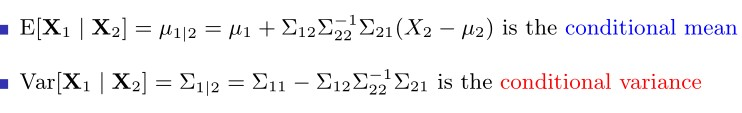
\includegraphics{appendix_images/inverse_lemma.jpg}
the theorem says toi ocnsider a multivariate gaussian a vector 1 and a vector 2 each vecto compinent has a mena and a covarianc matrix, this by lemma gives us the expression and the math behind is no tremendous, but it is long. What it is important is to undestand fto go from a joont to a conditional distribution in our case. thats i the value od the theorem.

One background further thing: assume that we have a gaussian variable distribution that we want to sample fromm, we had now ewe are going to do the opposite, before we had poitns and we tried to figure out the curve, now we have the curve and we are gointg to try to rpoduce data. I need to be able to draw sample froma gaussian distribution. i will assume that i have a meachnism that produces a uniform samples, so you have a random numebr generatior with equal probabolity from 0 to 1, I assume a also the cumulative aof a gaussian.

the cumulative of a gaussian is what you get if you syrta summing the area under the curve of the gaussian as you move from the left. value after valure you can plot the cumulative ahead (see figure) the point where there is a flex point is the mean beacuse tha gassias is symmetric. The asymptot is 1 becuase the are under the curve sumes to 1.
If i can draw a random number form Uniform and the project it to thre cumulative and then finally projct it back to the gaussian distribution. Inverse cumulative mapping. If oyu do this multiple times you are going to have many sample palced next to the mean and as sparse as the variance. in this process of sampling try to sample a point i froma gaussian that has mean 0 a variance 1, now letes try to draw a point from a gaussian with mean mu and variance sigma. \ldots{}

In the multivariate case suppose that we have evctor with two variables how do i draw a vector from a multivariate gasussian with 0 means and plot 1 covarianc ematrix. the theormeem also says that the marginal distribution can be seen by civariance matrix , fist take the men\_1 and take upper left element from the covariance matrix obtaining the marginal rpobabiloty for x\_1, i.e.

\[
\pi(x_1) = \mathbf{N}(\mu_1, \Sigma_{11}) \\
\pi(x_2) = \mathbf{N}(\mu_2, \Sigma_{22}) 
\]
then in our problem:

\[
\pi(x_1) = \mathbf{N}(0, 1) \\
\pi(x_2) = \mathbf{N}(0, 1) 
\]
Then for simplicity we can simplyfy by groupign vector into:
(vectore exoression multivariate)

I need a wau to take square trotto of matrices, if x come sfroma MVG

35:01--

  \bibliography{refs.bib,Rpackages.bib}

\end{document}
